%QQQ Below: "10pt" prints in 10-point. "12pt" prints in larger 12-point.
\documentclass[12pt,letterpaper]{article}
\usepackage{amsthm,amssymb,amsmath}
\usepackage[pdftex]{hyperref}
\usepackage{tikz}
\usepackage{subcaption}
\usepackage{adjustbox}
%QQQ To print single-spaced, comment out the line below (precede it with a "%").
%QQQ To print double-spaced, remove the "%" at the beginning of the line.
%\renewcommand{\baselinestretch}{2}

% TIKZ

\pgfdeclarelayer{bg}    % declare background layer
\pgfsetlayers{bg,main}  % set the order of the layers

\tikzset{every label/.append style={fill=white}}
\tikzset{
    every node/.style={circle, inner sep=0mm, draw, minimum size=5mm, scale=.85}
}
\tikzset{every label/.style={shape=rectangle, draw=none, fill=white}}

% MARGINS

\setlength{\textwidth}{6.3in}
\setlength{\textheight}{8.7in}
\setlength{\topmargin}{0pt}
\setlength{\headsep}{0pt}
\setlength{\headheight}{0pt}
\setlength{\oddsidemargin}{0pt}
\setlength{\evensidemargin}{0pt}

% SET UP SECTION NUMBERING

\setcounter{secnumdepth}{1}
% Number sections, but not subsections

% BREAK THEOREM STYLE

\newtheoremstyle{break}% name
  {}%         Space above, empty = `usual value'
  {}%         Space below
  {}% Body font
  {}%         Indent amount (empty = no indent, \parindent = para indent)
  {\bfseries}% Thm head font
  {.}%        Punctuation after thm head
  {\newline}% Space after thm head: \newline = linebreak
  {}%         Thm head spec

% DEFINE THEOREM-LIKE STRUCTURES

\theoremstyle{plain}
\newtheorem{lemma}{Lemma}[section]           % L:
%\newtheorem{lemma}{Lemma}                    % L:
\newtheorem{proposition}[lemma]{Proposition} % P:
\newtheorem{theorem}[lemma]{Theorem}         % T:
\newtheorem{corollary}[lemma]{Corollary}     % C:
\newtheorem{conjecture}[lemma]{Conjecture}   % J:
\newtheorem{question}[lemma]{Question}       % Q:
\newtheorem{problem}[lemma]{Problem}         % B:

\newtheorem{observation}[lemma]{Observation} % O:
\newtheorem{remark}[lemma]{Remark}           % R:

\theoremstyle{definition}
\newtheorem{definition}[lemma]{Definition}   % D:
\newtheorem{example}[lemma]{Example}         % E:

\theoremstyle{break}
\newtheorem{algorithm}[lemma]{Algorithm}     % A:
\newtheorem{implementation}[lemma]{Implementation}     % A:

% Also: Section = S:, Figure = Fig:, Item = It:, Equation = Eq:

% CHANGE APPEARANCE OF ENUMERATED LISTS

\renewcommand{\labelenumi}{(\roman{enumi})} % Labels (i), (ii), etc.

% CHANGE QED-RELATED COMMANDS

\renewcommand{\qed}{}
\newcommand{\ggcqedsymbol}{$\square$}
\newcommand{\ggcqed}{\hbox{}\nobreak\hbox{\quad\ggcqedsymbol}}
\newcommand{\ggcendpf}{\ggcqed}
%\newcommand{\ggcnopf}{}
\newcommand{\ggcnopf}{\ggcqed}
%\newcommand{\ggcendexample}{}
\newcommand{\ggcendexample}{\ggcqed}

% SET STYLE FOR DEFINED TERMS

\newcommand{\defterm}[1]{\emph{#1}} % Defined term
\newcommand{\abstdefterm}[1]{#1} % Defined term in abstract
\newcommand{\localdefterm}[1]{\emph{#1}} % Defined term used only nearby

% RUN-IN HEADINGS

\newcommand{\runinhead}[1]{\vskip0.1in\textbf{#1}} % Run-in heading
% This should be used at the start of a paragraph,
%  with no space between it and the first word of the paragraph.

% DEFINITIONS SPECIFIC TO THIS DOCUMENT

% (NONE)

\date{December 5, 2024}

\title{Path-Coloring Algorithms for Plane Graphs}

\author{Aven Bross\\
\small Department of Computer Science\\
\small University of Alaska\\
\small Fairbanks, AK 99775-6670\\
\small\texttt{dabross@alaska.edu} \and
Glenn G.~Chappell\\
\small Department of Computer Science\\
\small University of Alaska\\
\small Fairbanks, AK 99775-6670\\
\small\texttt{chappellg{@}member.ams.org} \and
Chris Hartman\\
\small Department of Computer Science\\
\small University of Alaska\\
\small Fairbanks, AK 99775-6670\\
\small\texttt{cmhartman{@}alaska.edu}}

\begin{document}

\maketitle
\centerline{\small \textit{2010 Mathematics Subject Classification.}
 Primary 05C38; Secondary 05C10, 05C15.}
\centerline{\small \textit{Key words and phrases.}
 Path coloring, list coloring, algorithm.}

\begin{abstract}
A \abstdefterm{path coloring} of a graph $G$ is a vertex coloring
of $G$ such that each color class induces a disjoint union of paths.
We present two efficient algorithms
to construct a path coloring of a plane graph.

The first algorithm, based on a proof of Poh, %\cite{Poh1990}
is given a plane graph;
it produces a path coloring of the given graph
using three colors.

The second algorithm,
based on similar proofs
by Hartman % \cite{Har1997}
and \v{S}krekovski, %\cite{Skr1999}
performs a list-coloring generalization of the above.
The algorithm is given a plane graph and an assignment of lists of
three colors to each vertex;
it produces a path coloring of the given graph
in which each vertex receives a color from its list.

Implementations are available for all algorithms that are described.
\end{abstract}

\section{Introduction}

All graphs will be finite, simple, and undirected.
See West~\cite{Wes2000} for graph theoretic terms.

A \defterm{path coloring} of a graph $G$ is a vertex coloring
(not necessarily proper) of $G$ such that each color class induces
a disjoint union of paths.
A graph $G$ is \defterm{path $k$-colorable} if $G$
admits a path coloring using $k$ colors.

Broere \& Mynhardt conjectured~\cite[Conj.~16]{BrMy1985}
that every planar graph is path $3$-colorable.
This was proven independently by Poh~\cite[Thm.~2]{Poh1990}
and by Goddard~\cite[Thm.~1]{God1991}.

\begin{theorem}[Poh 1990, Goddard 1991]\label{T:planar3c}
If $G$ is a planar graph,
then $G$ is path $3$-colorable.\ggcnopf\end{theorem}

It is easily shown that the ``$3$'' in Theorem~\ref{T:planar3c}
is best possible.
In particular, Chartrand \& Kronk~\cite[Section~3]{ChKr1969}
gave an example of a planar graph whose vertex set cannot be partitioned
into two subsets, each inducing a forest.

Hartman~\cite[Thm.~4.1]{Har1997}
proved a list-coloring generalization of Theorem~\ref{T:planar3c}
(see also Chappell \& Hartman~\cite[Thm.~2.1]{ChHa2017prep}).
A graph $G$ is \defterm{path $k$-choosable} if,
whenever each vertex of $G$ is assigned a list of $k$ colors,
there exists a path coloring of $G$ in which each vertex receives
a color from its list.

\begin{theorem}[Hartman 1997]\label{T:planar3}
If $G$ is a planar graph,
then $G$ is path $3$-choosable.\ggcnopf\end{theorem}

Essentially the same technique was used by
\v{S}krekovski~\cite[Thm.~2.2b]{Skr1999}
to prove a result slightly weaker than Theorem~\ref{T:planar3}.


\medskip

We discuss two efficient path-coloring algorithms
based on proofs of the above theorems.
We distinguish between a \defterm{planar} graph---one that
can be drawn in the plane without crossing edges---and
a \defterm{plane} graph---a graph with a given embedding
in the plane.

In Section~2 we outline our graph representations
and the basis for our computations of time complexity.

Section~3 covers an algorithm
based on Poh's proof of Theorem~\ref{T:planar3c}.
The algorithm is given a plane graph;
it produces a path coloring of the given graph
using three colors.

Section~4 covers an algorithm
based Hartman's proof of Theorem~\ref{T:planar3},
along with the proof of \v{S}krekovski mentioned above.
The algorithm is given a plane graph
and an assignment of a list of three colors to each vertex;
it produces a path coloring of the given graph
in which each vertex receives a color from its list.

Section~5 provides benchmark results for implementations of each
algorithm~\cite{Bro2017}. The section also
discusses how each algorithm may be modified to benefit from parallelism.

\section{Graph Representations and Time Complexity}

We will represent a graph via \textit{adjacency lists}:
a list, for each vertex $v$, of the neighbors of $v$.
A vertex can be represented by an integer $0\dots n-1$,
where $n=n(G)$ is the order of the graph.

A plane graph will be specified via
a \defterm{rotation scheme}:
a circular ordering,
for each vertex $v$, of the edges incident with $v$,
in the order they appear around $v$ in the plane embedding;
this completely specifies
the combinatorial embedding of the graph.
Rotation schemes are convenient when we represent a graph
using adjacency lists;
we simply order the adjacency
list for each vertex $v$ in counter-clockwise order around $v$;
no additional data structures are required.

A plane graph is \defterm{triangulated} if every face is a $3$-cycle, and
\defterm{weakly triangulated} if every face other than the
outer face is a $3$-cycle.
A graph $G$ is \defterm{connected} if given any $u,v\in G$, there exists a $u,v$-path in $G$.
We say that $G$ is \defterm{$n$-connected} if removing any $n-1$ vertices results in a
connected graph. The outer face of a plane graph that is both $2$-connected
and weakly triangulated is a path if $n=1$ or $n=2$, and a cycle if $n\ge 3$. 

The input for each algorithm will be a $2$-connected,
weakly triangulated plane graph with $n$ vertices and $m$ edges, represented
via adjacency lists. The input size will be $n$, the number of vertices. Note
that $\mathcal{O}(m)=\mathcal{O}(n)$, so it is equivalent to take the input size
to be $m$, the number of edges. Moreover, arbitrary simple planar graphs may be
plane embedded and triangulated in $\mathcal{O}(n)$ time, see Boyer and
Myrvold~\cite{BoMy2004}.

In Section~4, given an edge $uv$, we will need a constant time operation to
find $v$'s entry in $u$'s adjacency list from $u$'s entry in $v$'s list.
We define an \defterm{augmented adjacency list} to be an adjacency list such
that for
every edge $uv$ a reference to $v$'s entry in
$u$'s list is stored in $u$'s entry in $v$'s list, and vice versa. Given an
adjacency list representation of a graph, an augmented
adjacency list representation may be constructed in $\mathcal{O}(m)$ time via
the following procedure.

\begin{algorithm}\label{A:augment}
\textbf{Input.} An adjacency list representation Adj of a graph $G$.

\textbf{Output.} An augmented adjacency list representation AugAdj of
$G$ with the same rotation scheme as Adj.

\textbf{Step 1.} Construct an augmented adjacency list representation AugAdj
with the same rotation scheme as Adj, leaving the reference portion of each
entry uninitialized.

\textbf{Step 2.} For each vertex $v$ construct an array $\text{Wrk}[v]$
of vertex-reference pairs with length $\text{deg}(v)$. For each $v$ from
$0$ to $n-1$ iterate through
$\text{AugAdj}[v]$. For each neighbor $u$ in $\text{AugAdj}[v]$ append the pair
$(v,r_v(u))$ to
$\text{Wrk}[u]$, where $r_v(u)$ is a reference to $u$'s entry in
$\text{AugAdj}[v]$.

\textbf{Step 3.} For each $v$ from $n-1$ to $0$ iterate through
$\text{Wrk}[v]$. Upon reaching a pair $(u,r_u(v))$ in $\text{Wrk}[v]$ the
last element of $\text{Wrk}[u]$ will be $(v,r_v(u))$; for details on why this
must be the case, see the paragraph below. Use
$r_u(v)$ and $r_v(u)$ to look up and assign references for the edge $uv$ in
AugAdj$[u]$ and AugAdj$[v]$. Remove $(v,r_v(u))$ from the back of
$\text{Wrk}[u]$.
\end{algorithm}

After completing Step $2$ in Algorithm~\ref{A:augment} the array $\text{Wrk}[v]$
will contain
a pair $(u,r_u(v))$ for each neighbor $u$ of $v$, sorted in increasing order by
the neighbor $u$.
Suppose that $v$ is the current vertex at a given iteration of Step $3$ in
Algorithm~\ref{A:augment}. For each edge $uw\in E(G)$ such that
$u<w$ and $v<w$, prior iterations of Step 3 will have initialized the
references for $uw$ in $\text{AugAdj}[u]$ and $\text{AugAdj}[w]$, and also
removed the pair
$(w,r_w(u))$ from $\text{Wrk}[u]$. Therefore for each $(u,r_u(v))$ in
$\text{Wrk}[v]$, the array $\text{Wrk}[u]$ will contain only entries for
vertices $w$ where $w\le v$. Since $\text{Wrk}[u]$ is sorted in
increasing order by the neighboring vertices, the last element of
$\text{Wrk}[u]$ must be $(v,r_v(u))$.

\section{Path Coloring}

In this section we describe a linear time algorithm to path $3$-color
plane graphs. Let's first recount Poh's path $3$-coloring proof strategy.
Given a cycle $C$ in a plane graph $G$ we define $\text{Int}(C)$ to
be the subgraph of $G$ consisting of $C$ and all vertices and edges interior to
$C$. If $C$ is a length $1$ or $2$ path, we define $\text{Int}(C)=C$.
Equivalently, $\text{Int}(C)$ is the maximal $2$-connected subgraph of $G$ with
outer face $C$.

\begin{lemma}[Poh 1990]\label{L:planar3c}
Let $G$ be a $2$-connected, weakly triangulated plane graph with outer face
$C$. Let $c:V(C)\to S\subsetneq\{1,2,3\}$ be a $2$-coloring of $C$ such
that each color class induces a nonempty path. There exists an extension of
$c$ to a path $3$-coloring $c:V(G)\to\{1,2,3\}$ such that for each $v\in G-C$, if $vu\in
E(G)$ with $u\in C$, then $c(v)\ne c(u)$.
\end{lemma}

\begin{proof}
If $n(G)\le 3$, then $G=C$ and the path $2$-coloring of $C$ is a path
$3$-coloring of $G$. We proceed by induction on the order of $G$. 

Let $P_1,P_2$ be the two paths induced by the $2$-coloring of the outer face
$C$. 
Label the vertices of the outer face $C=v_1,v_2,\ldots, v_k$ in clockwise
order such that $P_1=v_1,v_2,\ldots, v_\ell$ and
$P_2=v_{l+1},v_{l+2},\ldots, v_k$.

Suppose $C$ is an induced subgraph of $G$. Let
$u,w\in V(G)-V(C)$ be the vertices such that $u,v_1,v_k$ and $w,v_\ell,v_{\ell+1}$
are faces of $G$; note that
$u$ and $w$ are uniquely determined, but it may be that $u=w$. Since
$C$ is an induced cycle in $G$ and $G\ne C$, $G-C$ is connected.
Let $P_3=u_1,u_2,\ldots,u_r$ be a $u,w$-path in $G-C$ of minimal length, and
note that $P_3$ is an induced subgraph of $G-C$.

Color each vertex of $P_3$ with the color in $\{1,2,3\}- S$ not used
in the $2$-coloring of
$C$. Let $C_1=v_1,v_2,\ldots,v_\ell,u_r,u_{r-1},\ldots,u_1$ and
$C_2=u_1,u_2,\ldots,u_r,v_{\ell+1},v_{l+2},\ldots,v_k$. The subgraphs
$\text{Int}(C_1)$ and $\text{Int}(C_2)$ together with the coloring $c$
each satisfy the requirements of the lemma. By the inductive hypothesis
there exist extensions of $c$ to a path
$3$-coloring of $\text{Int}(C_1)$ and a path $3$-coloring of $\text{Int}(C_2)$.
Since $\text{Int}(C_1)$ and $\text{Int}(C_2)$ only share the vertices in $P_3$
on their respective outer faces, the colorings agree and form a path
$3$-coloring of $G$.

Suppose $C$ is not an induced subgraph. Then there
exists an edge $v_iv_j\in E(G)-E(C)$ such that $i\le \ell < j$. Let
$C_1=v_1,v_2,\ldots,v_i,v_j,v_{j+1},\ldots,v_k$
and $C_2=v_i,v_{i+1},\ldots,v_j$.
By the inductive hypothesis, there exists an extension of $c$ to a path
$3$-coloring of $\text{Int}(C_1)$ and $\text{Int}(C_2)$. Again
the subgraphs only share vertices on their outer faces, and thus the
colorings agree and combine form a path $3$-coloring of $G$.\ggcnopf
\end{proof}

\begin{figure}[ht]
\begin{center}
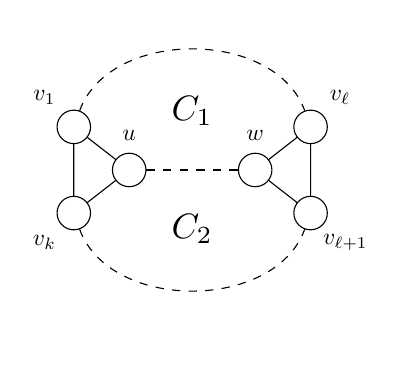
\begin{tikzpicture}[scale=1.6]
    \node (p0)[label=above left:${v_1}$] at (160:1.0cm) {};
    \node (pn) [label=above right:${v_\ell}$] at (20:1.0cm) {};
    \node (q0) [label=below left:${v_k}$] at (200:1.0cm) {};
    \node (qn) [label=below right:${v_{\ell+1}}$] at (340:1.0cm) {};
  \node (t0) [label=above:$u$] at (180:0.5cm) {};
  \node (t1) [label=above:$w$] at (0:0.5cm) {};
    \node (null) [draw=none, fill=none] at (270:1.25cm) {};
  
  \node (C1) [scale=1.5] [draw=none, fill=none] at (90:0.47cm) {$C_1$};
  \node (C2) [scale=1.5] [draw=none, fill=none] at (270:0.47cm) {$C_2$};
  
  \draw (p0) edge [bend left=70] (pn) [dashed];
  \draw (q0) edge [bend right=70] (qn) [dashed];
  \draw (p0) edge (q0);
  \draw (pn) edge (qn);
  \draw (p0) edge (t0);
  \draw (q0) edge (t0);
  \draw (pn) edge (t1);
  \draw (qn) edge (t1);
  \draw (t0) edge (t1) [dashed];
\end{tikzpicture}
$\qquad$
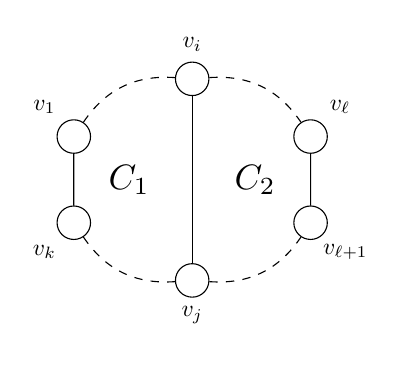
\begin{tikzpicture}[scale=1.6]
    \node (p0) [label=above left:${v_1}$] at (160:1.0cm) {};
    \node (p1) [label=above:${v_i}$] at (90:0.8cm) {};
    \node (pn) [label=above right:${v_\ell}$] at (20:1.0cm) {};
    \node (q0) [label=below left:${v_k}$] at (200:1.0cm) {};
    \node (q1) [label=below:${v_j}$] at (270:0.8cm) {};
    \node (qn) [label=below right:${v_{\ell+1}}$] at (340:1.0cm) {};
    \node (null) [draw=none, fill=none] at (270:1.25cm) {};
  
    \node (C1) [scale=1.5] [draw=none, fill=none] at (180:0.5cm) {$C_1$};
    \node (C2) [scale=1.5] [draw=none, fill=none] at (0:0.5cm) {$C_2$};
  
  \draw (p0) edge [bend left] (p1) [dashed];
  \draw (p1) edge [bend left] (pn) [dashed];
  \draw (q0) edge [bend right] (q1) [dashed];
  \draw (q1) edge [bend right] (qn) [dashed];
  \draw (p0) edge (q0);
  \draw (pn) edge (qn);
  \draw (p1) edge (q1);
\end{tikzpicture}
\caption{The proof of Lemma~\ref{L:planar3c} when $C$ is induced (left) and not
induced (right).}
\label{poh_figure}
\end{center}
\end{figure}

Let $G$ be a triangulated plane graph. We may trivially path $2$-color the outer
triangle. Applying Lemma~\ref{L:planar3c} extends this coloring to a path
$3$-coloring of $G$.

For an arbitrary planar graph $G$ we may compute an embedding and add edges
to produce a triangulated plane graph $G'$. Any path $3$-coloring of
$G'$ will also be a path $3$-coloring of $G$. Thus Theorem~\ref{T:planar3c}
follows from Lemma~\ref{L:planar3c}.

In the construction of the path $P_3$ in Poh's proof, the
induced $u,w$-path was picked to be a $u,w$-path of shortest length.
Thus a natural way to implement Poh's algorithm is to locate $u$,
and then use a breadth-first search
to construct a $u,w$-path and/or locate
a chord edge.

\begin{algorithm}\label{A:poh_bfs}
\textbf{Input.} Let $C=v_1,v_2,\ldots,v_k$ be a cycle in a $2$-connected,
weakly triangulated plane
graph $G$ with adjacency list representation $\text{Adj}$. Let 
$c$ be an array of colors representing a $2$-coloring of $C$ such
that each color class induces a path, respectively labelled
$P_1=v_1,v_2,\ldots,v_\ell$ and $P_2=v_\ell,v_{\ell+1},\ldots,v_k$. Assume that
$c[v]=0$ for each $v\in\text{Int}(C)-C$.

\textbf{Output.} For each vertex $v\in\text{Int}(C)-C$, a nonzero color will be
assigned to $c[v]$ such that $c$ represents a path $3$-coloring of
$\text{Int}(C)$ extending the original $2$-coloring of $C$. Moreover, if
$v\in \text{Int}(C)-C$ has a neighbor $u\in C$, then $c[v]\ne c[u]$.

\textbf{Base case.} If $k=3$, then $C=\text{Int}(C)$ and $G$ is colored.

\textbf{Recursive step.} Iterate through $\text{Adj}[v_1]$ to locate the vertex $u$
immediately counter-clockwise from $v_k$. Note that since $G$ is triangulated,
$v_1,u,v_k$ is a face of $G$.

\textbf{Case 1.} Suppose that $c[u]\ne 0$. If $c[u]=c[v_k]$,
then $u\in P_2$ and
thus $u=v_{k-1}$ since $G$ is
triangulated and $P_2$ is an induced path. Recursively
apply the algorithm to the cycle $C'=v_1,v_2,\ldots,v_{k-1}$.

Otherwise $c[u]=c[v_1]$, and it must be that $u=v_2\in P_1$. Recursively
apply the algorithm to the cycle $C'=v_2,v_3,\ldots,v_{k-1}$.

\textbf{Case 2.} Suppose that $c[u]=0$ and therefore $u\in \text{Int}(C)-C$.
Perform a breadth-first search of $\text{Int}(C)-C$ starting from the
vertex $u$. Terminate the search upon locating a vertex $w$ with
adjacent
neighbors $v_i\in P_1$ and $v_j\in P_2$ such that $i\ne 1$ or $j\ne k$.

Backtrack along the breadth-first search tree
to construct a $u,w$-path of minimum length $P_3=u_1,u_2,\ldots,u_r$.
Color the vertices in
$P_3$ with the third color not used in the $2$-coloring of $C$.
Define
$$C_1=v_1,v_2,\ldots,v_i,u_r,u_{r-1},\ldots,u_1 \text{ and }
C_2=u_1,u_2,\ldots,u_r,v_j,v_{j-1},\ldots,v_k.$$
Apply the algorithm
separately to $C_1$ and $C_2$. If $i=\ell$ and $j={\ell+1}$, then $C$ was an
induced cycle and we are done. Otherwise, also apply the algorithm to
$C_3=v_i,v_{i+1},\ldots,v_j$.
\end{algorithm}

\begin{figure}[ht]
\begin{center}
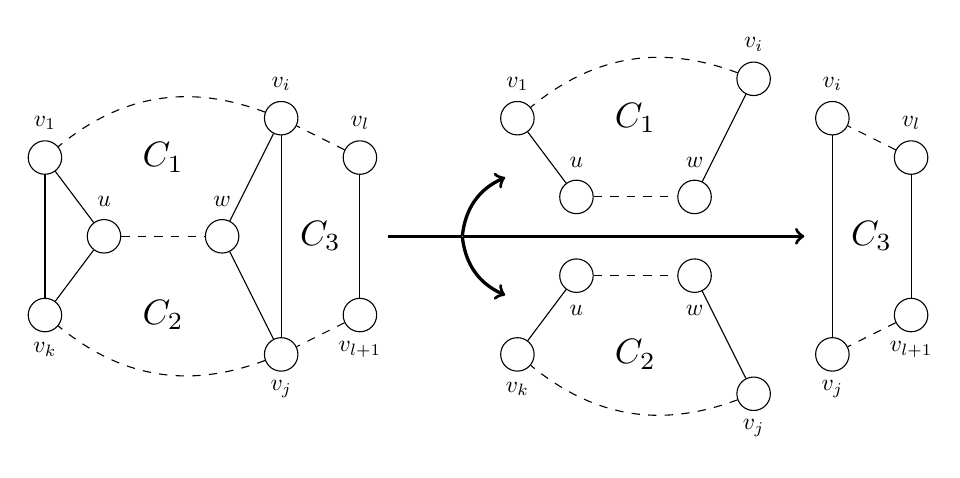
\begin{tikzpicture}
  \node (vl) [label=above:$v_l$] at (2cm, 1cm) {};
  \node (v1) [label=above:$v_1$] at (-2cm, 1cm) {};
  \node (vl1) [label=below:$v_{l+1}$] at (2cm, -1cm) {};
  \node (vk) [label=below:$v_k$] at (-2cm, -1cm) {};
  \node (w) [label=above:$w$] at (0.25cm, 0cm) {};
  \node (u) [label=above:$u$] at (-1.25cm, 0cm) {};
  \node (vi) [label=above:$v_i$] at (1cm, 1.5cm) {};
  \node (vj) [label=below:$v_j$] at (1cm, -1.5cm) {};
  
  \node (CP) [scale=1.5] [draw=none, fill=none] at (-0.5cm, 1cm) {$C_1$};
  \node (CQ) [scale=1.5] [draw=none, fill=none] at (-0.5cm, -1cm) {$C_2$};
  \node (Ci) [scale=1.5] [draw=none, fill=none] at (1.5cm, 0cm) {$C_3$};
  
  \node (null) [draw=none, fill=none] at (270:2.5cm) {};
  
  \draw (vl) edge (vi) [dashed];
  \draw (vi) edge [bend right] (v1) [dashed];
  \draw (vl1) edge (vj) [dashed];
  \draw (vj) edge [bend left] (vk) [dashed];
  \draw (vl) edge (vl1);
  \draw (v1) edge (vk);
  \draw (vi) edge (vj);
  \draw (v1) edge (u);
  \draw (vk) edge (u);

  \draw (u) edge (w) [dashed];
  \draw (vi) edge (w);
  \draw (vj) edge (w);

  \node (bs) at (2.35cm, 0.0cm) [draw=none, fill=none, minimum size=0mm] {};
  \node (bm) at (3.3cm, 0.0cm) [draw=none, fill=none, minimum size=0mm] {};
  \node (be1) at (3.85cm, 0.75cm) [draw=none, fill=none, minimum size=0mm] {};
  \node (be2) at (3.85cm, -0.75cm) [draw=none, fill=none, minimum size=0mm] {};
  \node (be3) at (7.65cm, 0.0cm) [draw=none, fill=none, minimum size=0mm] {};

  \draw (bs) edge [very thick] (bm);
  \draw (bm) edge[very thick, ->, bend left] (be1);
  \draw (bm) edge[very thick, ->, bend right] (be2);
  \draw (bm) edge[very thick, ->] (be3);

  \node (p0) [label=above:$v_l$] at (9cm, 1cm) {};
  \node (q0) [label=below:$v_{l+1}$] at (9cm, -1cm) {};
  \node (pi) [label=above:$v_i$] at (8cm, 1.5cm) {};
  \node (qj) [label=below:$v_j$] at (8cm, -1.5cm) {};
  
  \node (pi_1) [label=above:$v_i$] at (7cm, 2cm) {};
  \node (pn) [label=above:$v_1$] at (4cm, 1.5cm) {};
  \node (t0) [label=above:$w$] at (6.25cm, 0.5cm) {};
  \node (t1) [label=above:$u$] at (4.75cm, 0.5cm) {};
  
  \node (CP) [scale=1.5] [draw=none, fill=none] at (5.5cm, 1.5cm) {$C_1$};
  \node (CQ) [scale=1.5] [draw=none, fill=none] at (5.5cm, -1.5cm) {$C_2$};
  \node (Ci) [scale=1.5] [draw=none, fill=none] at (8.5cm, 0cm) {$C_3$};
  
  \node (qj_1) [label=below:$v_j$] at (7cm, -2cm) {};
  \node (qn) [label=below:$v_k$] at (4cm, -1.5cm) {};
  \node (t0_1) [label=below:$w$] at (6.25cm, -0.5cm) {};
  \node (t1_1) [label=below:$u$] at (4.75cm, -0.5cm) {};

  \draw (p0) edge (pi) [dashed];
  \draw (pi_1) edge [bend right] (pn) [dashed];
  \draw (q0) edge (qj) [dashed];
  \draw (qj_1) edge [bend left] (qn) [dashed];
  \draw (p0) edge (q0);
  \draw (pi) edge (qj);
  \draw (pn) edge (t1);
  \draw (qn) edge (t1_1);
  \draw (t1) edge (t0) [dashed];
  \draw (t1_1) edge (t0_1) [dashed];
  \draw (pi_1) edge (t0);
  \draw (qj_1) edge (t0_1);
\end{tikzpicture}
\caption{Dividing $G$ along the edge $v_iv_j$ and the $uw$-path $P_3$ in
Algorithm~\ref{A:poh_bfs}.}
\end{center}
\end{figure}

\begin{figure}[ht]
\begin{center}
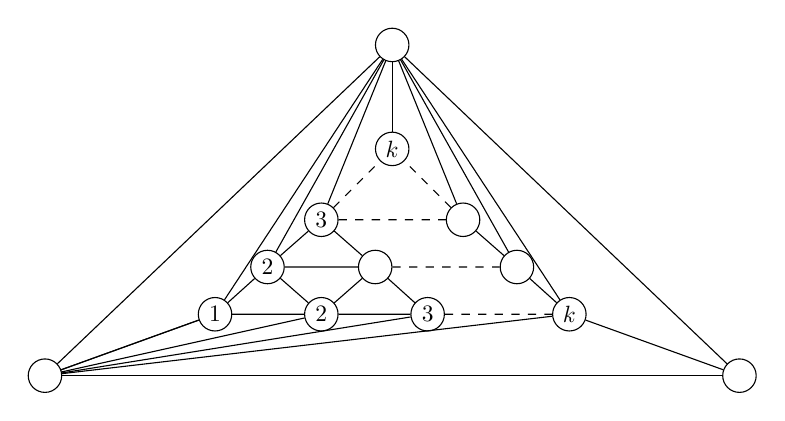
\begin{tikzpicture}[scale=1.2]
  \node (t1) at (0cm, 3.5cm) {};
  \node (t2) at (3.675cm, 0cm) {};
  \node (t3) at (-3.675cm, 0cm) {};

  \node (k1) at (-1.875cm, 0.65cm) {$1$};
  \node (k2) at (-0.75cm, 0.65cm) {$2$};
  \node (k3) at (0.375cm, 0.65cm) {$3$};
  \node (kn) at (1.875cm, 0.65cm) {$k$};

  \node (l1) at (-1.32cm, 1.15cm) {$2$};
  \node (l2) at (-0.18cm, 1.15cm) {};
  \node (ln) at (1.32cm, 1.15cm) {};

  \node (j1) at (-0.75cm, 1.65cm) {$3$};
  \node (jn) at (0.75cm, 1.65cm) {};

  \node (p) at (0cm, 2.4cm) {$k$};

  \begin{pgfonlayer}{bg}
	  \draw (t1) edge (t2); \draw (t3) edge (t2); \draw (t1) edge (t3);
	  \draw (k1) edge (k2); \draw (k3) edge (k2);
	  \draw (k3) edge (kn) [dashed];

	  \draw (l1) edge (l2);
	  \draw (l2) edge (ln) [dashed];

	  \draw (j1) edge (jn) [dashed];

	  \draw (j1) edge (p) [dashed];
	  \draw (jn) edge (p) [dashed];

	  \draw (t1) edge (k1); \draw (t1) edge (kn);
	  \draw (t1) edge (l1); \draw (t1) edge (ln);
	  \draw (t1) edge (p);
	  \draw (t2) edge (kn); \draw (t3) edge (k1);

	  \draw (k1) edge (l1); \draw (k2) edge (l1);
	  \draw (k2) edge (l2); \draw (k3) edge (l2);
	  \draw (kn) edge (ln);

	  \draw (l1) edge (j1); \draw (l2) edge (j1);
	  \draw (jn) edge (ln);

	  \draw (j1) edge (t1); \draw (jn) edge (t1);

	  \draw (t3) edge (k1); \draw (t3) edge (k2);
	  \draw (t3) edge (k3); \draw (t3) edge (kn);
  \end{pgfonlayer}
\end{tikzpicture}

\caption{The collection of graphs $\{G_k\}_{k\in\mathbb{N}}$ for which
Algorithm~\ref{A:poh_bfs} performs poorly.}\label{F:poh_bad_graph_collection}
\end{center}
\end{figure}

Unfortunately Algorithm~\ref{A:poh_bfs}
is not linear. Consider the family of
graphs $\{G_k\}_{k\in\mathbb{N}}$ depicted in
Figure~\ref{F:poh_bad_graph_collection}.
Fix $k\in\mathbb{N}$ and note that
$n=n(G_k)=k(k+1)/2+3$. Assume
that the outer triangle is path $2$-colored such that the top vertex is
assigned a color distinct from the bottom two. At depth $i$ of
Algorithm~\ref{A:poh_bfs}
the shortest path through the interior will be the path of length
$r=k-i+1$ directly along the base of the inner triangle. A breadth-first search
of this inner triangle will hit all $r(r+1)/2$ vertices in order to find this
path. Therefore the total number of operations performed will be
\[
    \Theta\left( \sum_{r=1}^k\frac{r(r+1)}{2} \right)=\Theta(n^{3/2}).
\]
So Poh's algorithm implemented with breadth-first search is $\Omega(n^{3/2})$.

However, the correctness of Poh's proof only relied on
locating some induced $u,w$-path.
We will show that there exists a linear time implementation of Poh's
algorithm that does not always find the shortest $u,w$-path.

For any subgraph $H$ of $G$, let $N(H)$ be the set of vertices in $V(G)$ with a
neighbor in $V(H)$. Our strategy will be to construct an induced
path $P_3=u_1,u_2,\ldots,u_d$ consisting of vertices in $N(P_1)-V(C)$.

\begin{algorithm}\label{A:poh_linear}
\textbf{Input.} Assume that $C=v_1,v_2,\ldots,v_k$ is an induced cycle in a
$2$-connected, weakly triangulated plane
graph $G$ with adjacency list representation $\text{Adj}$.

Let $c$ be a length $n$ array of colors
representing a $2$-coloring of $C$ such
that each color class induces a path, respectively $P_1=v_1,v_2,\ldots,v_i$ and
$P_2=v_{i+1},v_{i+2},\ldots,v_k$. Let $c_{P_1}$ and $c_{P_2}$ be the colors
for $P_1$ and $P_2$, respectively. Assume $c[v]=0$ for each
$v\in\text{Int}(C)-C$.

Let $S$ be a length $n$ array of integer marks and let $m_{P_1}$ be an integer
such that for each $v\in\text{Int}(C)-C$ we have $S[v]=m_{P_1}$ if and only if
$v\in N(P_1)$.

Let $u\in\text{Int}(C)-C$ be the unique vertex such that $v_1,u,v_k$ is a face.
The vertex $u$ and the entry for $v_k$ in $\text{Adj}[u]$, together
with $\text{Adj}$, $c$, and $S$, will serve as the concrete
representation of the algorithm input.

\textbf{Output.} For each vertex $v\in\text{Int}(C)-C$, a nonzero color will be
assigned to $c[v]$ such that $c$ represents a path $3$-coloring of
$\text{Int}(C)$ extending the original $2$-coloring of $C$. Moreover, if
$v\in N(P_1)-C$, then $c[v]\ne c_{P_1}$, and if $v\in N(P_2)-C$, then
$c[v]\ne c_{P_2}$.

\textbf{Procedure.} The algorithm will construct a $u,w$-path $P_3$
in $\text{Int}(C)-C$ such that for each $v\in P_3$, $S[v]=m_{P_1}$, that is,
$V(P_3)\subset N(P_1)$.
The vertex $w\in\text{Int}(C)-C$ is the unique vertex such that
$w,v_i,v_{i+1}$ is a face; $w$ will
not be known prior to constructing $P_3$.

Each vertex of the path $P_3$ will be colored with
$c_{P_3}\in\{1,2,3\}-\{c_{P_1},c_{P_2}\}$.
Each vertex in $N(P_3)-C-P_3$ will be marked with a new unique
mark $m_{P_3}$.

%While constructing
%the path $P_3$, we will locate each induced cycle formed by
%vertices in $V(P_1)\cup V(P_3)$, and each induced cycle formed by
%vertices in $V(P_2)\cup V(P_3)$, and
%make a recursive call on each cycle with a non-empty interior.

We will store $u_j$, the last
vertex added to $P_3=u_1,u_2,\ldots,u_j$, along with the entry for
$u_{j-1}$ in $\text{Adj}[u_j]$. Define $u_0=v_k$ for the purpose
of identifying $u_{j-1}$ when $j=1$. Track the
last edge
encountered between a vertex $u_r\in P_3$ and a vertex $v_s\in P_2$, represented
by $u_r$ and the entry for $v_s$ in $\text{Adj}[u_r]$.
Initialize $j\leftarrow 1$, $u_1\leftarrow u$, and $u_rv_s\leftarrow
uv_k$. 

\textbf{Step 1.} Iterate through the neighbors of $u_j$ in counter-clockwise
order, starting with
the neighbor immediately counter-clockwise from $u_{j-1}$.
Track an optional vertex $y\leftarrow\text{NULL}$ indicating
the neighbor of $u_j$ in $N(P_1)-C$ that will become
$u_{j+1}$ once all other the neighbors of $u_j$ have been handled. Also store
an optional edge $u_jv_\ell\leftarrow\text{NULL}$, represented by the entry
for $v_j$ in $\text{Adj}[u_j]$, indicating the last neighbor of $u_j$ in $P_1$
that was encountered. At each neighbor $v$ of $u_j$ one of the following cases
will be satisfied.

\textbf{Case 1.1.} Suppose that $u_jv_\ell=\text{NULL}$,
that is, no neighbor of $u_j$ in $P_1$ has been encountered yet.
See Figure~\ref{F:poh_linear_1} for a sketch of each sub-case.

\begin{figure}[ht]
\begin{center}
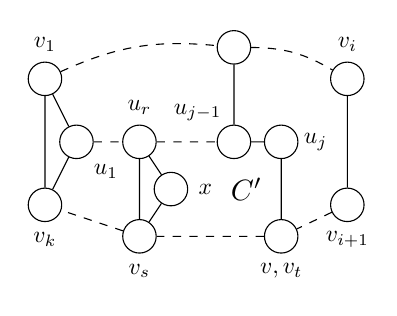
\begin{tikzpicture}[scale=1.6]
    \node (v1) [label=above:${v_1}$] at (-0.25cm, 1.0cm) {};
    \node (vp) at (1.25cm, 1.25cm) {};
    \node (vi) [label=above:${v_i}$] at (2.15cm, 1.0cm) {};
    \node (vi1) [label=below:${v_{i+1}}$] at (2.15cm, 0.0cm) {};
    \node (vs) [label=below:${v_{s}}$] at (0.5cm, -0.25cm) {};
    \node (vt) [label=below:${v,v_{t}}$] at (1.625cm, -0.25cm) {};
    \node (vk) [label=below:${v_k}$] at (-0.25cm, 0.0cm) {};
    \node (u1) [label=below right:${u_1}$] at (0.0cm, 0.5cm) {};
    \node (ur) [label=above:${u_r}$] at (0.5cm, 0.5cm) {};
    \node (uj1) [label=above left:${u_{j-1}}$] at (1.25cm, 0.5cm) {};
    \node (uj) [label=right:${u_j}$] at (1.625cm, 0.5cm) {};
    \node (x) [label=right:${x}$] at (0.75cm, 0.125cm) {};

    \node (C) [scale=1.25] [draw=none, fill=none] at (1.35cm, 0.125cm) {$C'$};

    \begin{pgfonlayer}{bg}
        \draw (v1) edge[dashed, bend left=15] (vp);
        \draw (vp) edge[dashed, bend left=15] (vi);
        \draw (vi) edge (vi1);
        \draw (vi1) edge [dashed] (vt);
        \draw (vt) edge [dashed] (vs);
        \draw (vs) edge [dashed] (vk);
        \draw (vk) edge (v1);
        \draw (v1) edge (u1);
        \draw (vs) edge (ur);
        \draw (vk) edge (u1);
        \draw (u1) edge[dashed] (ur);
        \draw (ur) edge[dashed] (uj1);
        \draw (uj1) edge (uj);
        \draw (uj) edge (vt);
        \draw (uj1) edge (vp);
        \draw (ur) edge (x);
        \draw (vs) edge (x);
    \end{pgfonlayer}
\end{tikzpicture}
$\quad$
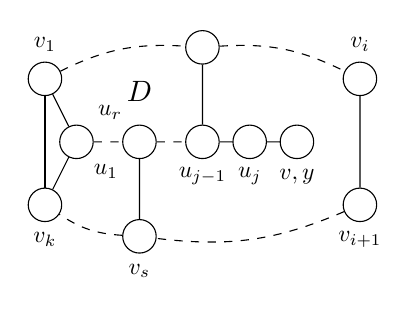
\begin{tikzpicture}[scale=1.6]
    \node (v1) [label=above:${v_1}$] at (0.0cm, 1.0cm) {};
    \node (vp) at (1.25cm, 1.25cm) {};
    \node (vi) [label=above:${v_i}$] at (2.5cm, 1.0cm) {};
    \node (vi1) [label=below:${v_{i+1}}$] at (2.5cm, 0.0cm) {};
    \node (vs) [label=below:${v_{s}}$] at (0.75cm, -0.25cm) {};
    \node (vk) [label=below:${v_k}$] at (0.0cm, 0.0cm) {};
    \node (u1) [label=below right:${u_1}$] at (0.25cm, 0.5cm) {};
    \node (ur) [label=above left:${u_r}$] at (0.75cm, 0.5cm) {};
    \node (uj1) [label=below:${u_{j-1}}$] at (1.25cm, 0.5cm) {};
    \node (uj) [label=below:${u_j}$] at (1.625cm, 0.5cm) {};
    \node (y) [label=below:${v,y}$] at (2.0cm, 0.5cm) {};

    \node (D) [scale=1.25] [draw=none, fill=none] at (0.75cm, 0.9cm) {$D$};

    \begin{pgfonlayer}{bg}
        \draw (v1) edge[dashed, bend left=15] (vp);
        \draw (vp) edge[dashed, bend left=15] (vi);
        \draw (vi) edge (vi1);
        \draw (vi1) edge[dashed, bend left=15] (vs);
        \draw (vs) edge[dashed, bend left=15] (vk);
        \draw (vk) edge (v1);
        \draw (v1) edge (u1);
        \draw (vs) edge (ur);
        \draw (vk) edge (u1);
        \draw (u1) edge[dashed] (ur);
        \draw (ur) edge[dashed] (uj1);
        \draw (uj1) edge (uj);
        \draw (uj) edge (y);
        \draw (uj1) edge (vp);
    \end{pgfonlayer}
\end{tikzpicture}
$\quad$
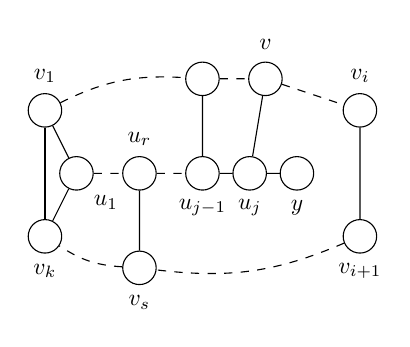
\begin{tikzpicture}[scale=1.6]
    \node (v1) [label=above:${v_1}$] at (0.0cm, 1.0cm) {};
    \node (vp) at (1.25cm, 1.25cm) {};
    \node (vi) [label=above:${v_i}$] at (2.5cm, 1.0cm) {};
    \node (vi1) [label=below:${v_{i+1}}$] at (2.5cm, 0.0cm) {};
    \node (vs) [label=below:${v_{s}}$] at (0.75cm, -0.25cm) {};
    \node (vk) [label=below:${v_k}$] at (0.0cm, 0.0cm) {};
    \node (u1) [label=below right:${u_1}$] at (0.25cm, 0.5cm) {};
    \node (ur) [label=above:${u_r}$] at (0.75cm, 0.5cm) {};
    \node (uj1) [label=below:${u_{j-1}}$] at (1.25cm, 0.5cm) {};
    \node (uj) [label=below:${u_j}$] at (1.625cm, 0.5cm) {};
    \node (y) [label=below:${y}$] at (2.0cm, 0.5cm) {};
    \node (v) [label=above:${v}$] at (1.75cm, 1.25cm) {};

    \begin{pgfonlayer}{bg}
        \draw (v1) edge[dashed, bend left=15] (vp);
        \draw (vp) edge[dashed] (v);
        \draw (v) edge[dashed] (vi);
        \draw (vi) edge (vi1);
        \draw (vi1) edge[dashed, bend left=15] (vs);
        \draw (vs) edge[dashed, bend left=15] (vk);
        \draw (vk) edge (v1);
        \draw (v1) edge (u1);
        \draw (vs) edge (ur);
        \draw (vk) edge (u1);
        \draw (u1) edge[dashed] (ur);
        \draw (ur) edge[dashed] (uj1);
        \draw (uj1) edge (uj);
        \draw (uj) edge (y);
        \draw (uj) edge (v);
        \draw (uj1) edge (vp);
    \end{pgfonlayer}
\end{tikzpicture}
\caption{Algorithm~\ref{A:poh_linear}, Case~1.1.2 (left), Case~1.1.3 (middle),
and Case~1.1.4 (right).}\label{F:poh_linear_1}
\end{center}
\end{figure}

\textbf{Case 1.1.1.} Suppose $c[v]=0$ and $S[v]\ne m_{P_1}$, that is,
$v\in\text{Int}(C)-C-N(P_1)$. Assign $S[v]\leftarrow m_{P_3}$.

\textbf{Case 1.1.2.} Suppose that $c[v]=c_{P_2}$, that is, $v=v_t\in P_2$.
Observe that $P_1'=u_r,u_{r+1},\ldots, u_j$ and $P_2'=v_s,v_{s+1},\ldots,v_t$
are colored induced paths that together with the edges $u_rv_s$ and $u_jv_t$
form an induced cycle $C'$. Moreover, the algorithm will have already marked
each vertex in $N_{P_3}\cap V(\text{Int}(C')-C')$ with $m_{P_3}$.
Let
$x$ be the neighbor of $u_r$ immediately counter-clockwise from $v_s$.
If $c[x]=0$, make a recursive call with $u'\leftarrow x$ and
$u'v_k'\leftarrow xv_s$ to path $3$-color $\text{Int}(C')$. Then assign
$u_rv_s\leftarrow u_jv_t$ to track that $u_jv_t$ is now the last edge between
$P_3$ and $P_2$ that we've encountered.

\textbf{Case 1.1.3.} Suppose that $c[v]=0$ and $S[v]=m_{P_1}$, that is,
$v\in N(P_1)-C$. If $y\ne\text{NULL}$, assign $S[v]\leftarrow m_{P_3}$.
Otherwise, assign $y\leftarrow v$ and color
$c[y]\leftarrow c_{P_3}$. We claim that $u_1,u_2,\ldots,u_j,y$ is an induced
path. Since $u_j\in N(P_1)$, there exists an edge $u_jv_t$ where $v_t\in P_1$.
Observe that $D=v_1,v_2,\ldots,v_t,u_j,u_{j-1},\ldots,u_1$ is a cycle in
$\text{Int}(C)$. Since $y\not\in\text{Int}(D)$, if an edge $yu_e$ exists with
$u_e\in P_3-u_j$,
then the entry for $y$ in $\text{Adj}[u_e]$ is between $u_{e-1}$ and
$u_{e+1}$ counter-clockwise.
But then $y$ would have been encountered before $u_{e+1}$
when iterating through $\text{Adj}[u_e]$, a contradiction since
$S[y]=m_{P_1}$.

\textbf{Case 1.1.4.} Suppose that $c[v]=c_{P_1}$, that is, $v\in P_1$.
Assign $u_jv_\ell\leftarrow u_jv$. If $y=\text{NULL}$, it must be
that $v=v_i\in P_1$ is the last vertex of $P_1$ and therefore $u_j=w$.
To see this, note
that the neighbor $a$ of $u_j$ immediately clockwise from $v$ is adjacent
to $v\in P_1$, but $a$ was not assigned to $y$. Therefore $c[a]=c_{P_2}$ and so
$a=v_{i+1}$ and $v=v_i$. Since $u_j,v_i,v_{i+1}$ is a face, $u_j=w$ by
definition.

\textbf{Case 1.2.} Suppose that $u_jv_\ell\ne\text{NULL}$. Let $z$ be
the neighbor of $u_j$ immediately counter-clockwise from $v_\ell$.
See Figure~\ref{F:poh_linear_2} for a sketch of each sub-case.

\begin{figure}[ht]
\begin{center}
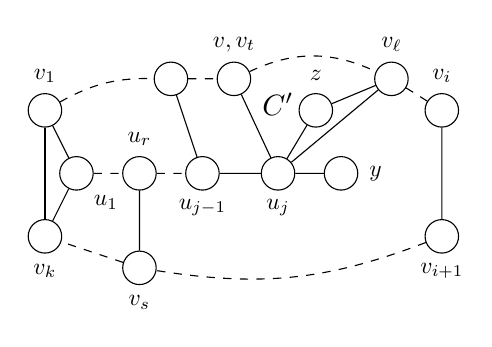
\begin{tikzpicture}[scale=1.6]
    \node (v1) [label=above:${v_1}$] at (0.0cm, 1.0cm) {};
    \node (vp) at (1.0cm, 1.25cm) {};
    \node (vi) [label=above:${v_i}$] at (3.15cm, 1.0cm) {};
    \node (vi1) [label=below:${v_{i+1}}$] at (3.15cm, 0.0cm) {};
    \node (vs) [label=below:${v_{s}}$] at (0.75cm, -0.25cm) {};
    \node (vt) [label=above:${v,v_{t}}$] at (1.5cm, 1.25cm) {};
    \node (vl) [label=above:${v_{\ell}}$] at (2.75cm, 1.25cm) {};
    \node (vk) [label=below:${v_k}$] at (0.0cm, 0.0cm) {};
    \node (u1) [label=below right:${u_1}$] at (0.25cm, 0.5cm) {};
    \node (ur) [label=above:${u_r}$] at (0.75cm, 0.5cm) {};
    \node (uj1) [label=below:${u_{j-1}}$] at (1.25cm, 0.5cm) {};
    \node (uj) [label=below:${u_j}$] at (1.85cm, 0.5cm) {};
    \node (y) [label=right:${y}$] at (2.35cm, 0.5cm) {};
    \node (z) [label=above:${z}$] at (2.15cm, 1.0cm) {};

    \node (C) [scale=1.25] [draw=none, fill=none] at (1.85cm, 1.05cm) {$C'$};

    \begin{pgfonlayer}{bg}
        \draw (v1) edge[dashed, bend left=15] (vp);
        \draw (vp) edge[dashed] (vt);
        \draw (vt) edge[dashed, bend left=25] (vl);
        \draw (vl) edge[dashed] (vi);
        \draw (vi) edge (vi1);
        \draw (vi1) edge [dashed, bend left=15] (vs);
        \draw (vs) edge [dashed] (vk);
        \draw (vk) edge (v1);
        \draw (v1) edge (u1);
        \draw (vs) edge (ur);
        \draw (vk) edge (u1);
        \draw (u1) edge[dashed] (ur);
        \draw (ur) edge[dashed] (uj1);
        \draw (uj1) edge (uj);
        \draw (uj) edge (vt);
        \draw (uj1) edge (vp);
        \draw (uj) edge (vl);
        \draw (uj) edge (y);
        \draw (uj) edge (z);
        \draw (vl) edge (z);
    \end{pgfonlayer}
\end{tikzpicture}
$\qquad$
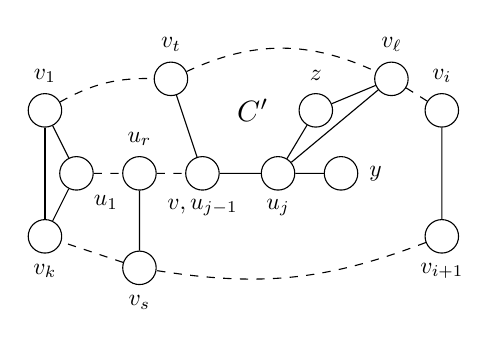
\begin{tikzpicture}[scale=1.6]
    \node (v1) [label=above:${v_1}$] at (0.0cm, 1.0cm) {};
    \node (vi) [label=above:${v_i}$] at (3.15cm, 1.0cm) {};
    \node (vi1) [label=below:${v_{i+1}}$] at (3.15cm, 0.0cm) {};
    \node (vs) [label=below:${v_{s}}$] at (0.75cm, -0.25cm) {};
    \node (vt) [label=above:${v_{t}}$] at (1.0cm, 1.25cm) {};
    \node (vl) [label=above:${v_{\ell}}$] at (2.75cm, 1.25cm) {};
    \node (vk) [label=below:${v_k}$] at (0.0cm, 0.0cm) {};
    \node (u1) [label=below right:${u_1}$] at (0.25cm, 0.5cm) {};
    \node (ur) [label=above:${u_r}$] at (0.75cm, 0.5cm) {};
    \node (uj1) [label=below:${v,u_{j-1}}$] at (1.25cm, 0.5cm) {};
    \node (uj) [label=below:${u_j}$] at (1.85cm, 0.5cm) {};
    \node (y) [label=right:${y}$] at (2.35cm, 0.5cm) {};
    \node (z) [label=above:${z}$] at (2.15cm, 1.0cm) {};

    \node (C) [scale=1.25] [draw=none, fill=none] at (1.65cm, 1.0cm) {$C'$};

    \begin{pgfonlayer}{bg}
        \draw (v1) edge[dashed, bend left=15] (vt);
        \draw (vt) edge[dashed, bend left=25] (vl);
        \draw (vl) edge[dashed] (vi);
        \draw (vi) edge (vi1);
        \draw (vi1) edge [dashed, bend left=15] (vs);
        \draw (vs) edge [dashed] (vk);
        \draw (vk) edge (v1);
        \draw (v1) edge (u1);
        \draw (vs) edge (ur);
        \draw (vk) edge (u1);
        \draw (u1) edge[dashed] (ur);
        \draw (ur) edge[dashed] (uj1);
        \draw (uj1) edge (uj);
        \draw (uj1) edge (vt);
        \draw (uj) edge (vl);
        \draw (uj) edge (y);
        \draw (uj) edge (z);
        \draw (vl) edge (z);
    \end{pgfonlayer}
\end{tikzpicture}
\caption{Algorithm~\ref{A:poh_linear}, Case~1.2.2 (left)
and Case~1.2.3 (right).}\label{F:poh_linear_2}
\end{center}
\end{figure}

\textbf{Case 1.2.1.} Suppose that $c[v]=0$, that is, $v\in\text{Int}(C)-C-P_3$.
Assign $S[v]\leftarrow m_{P_3}$.

\textbf{Case 1.2.2.} Suppose that $c[v]=c_{P_1}$, that is,
$v=v_t\in P_1$. Observe that $C'=u_j,v_t,v_{t+1},\ldots,v_\ell$ is an induced
cycle. Moreover,
the algorithm will have already marked each vertex in $N(P_3)\cap
V(\text{Int}(C')-C')$ with $m_{P_3}$.
If $c[z]=0$, make a recursive call with $u'\leftarrow z$ and
$u'v_k'\leftarrow zv_\ell$ to path $3$-color $\text{Int}(C')$.
Otherwise, $z=v$ and $\text{Int}(C')=C'$.

\textbf{Case 1.2.3.} Suppose that $c[v]\ne 0$ and $c[v]\ne c_{P_1}$.
Then it must
be that $c[v]= c_{P_3}$ and $v=u_{j-1}$. Choose the largest $t$ such that
$v_t\in P_1$ and $u_{j-1}v_{t}$ is an edge. Observe that
$C'=u_j,u_{j-1},v_t,v_{t+1},\ldots,v_\ell$ is an induced cycle. Moreover,
the algorithm will have marked each vertex in $N(P_3)\cap
V(\text{Int}(C')-C')$ with $m_{P_3}$.
If $c[z]=0$, make a recursive call with $u'\leftarrow z$ and
$u'v_k'\leftarrow zv_\ell$ to color $\text{Int}(C')$. Otherwise,
$z=v$ and $\text{Int}(C')=C'$.

\textbf{Step 2.} If $y\ne\text{NULL}$, then 
assign $j\leftarrow j+1$, $u_j\leftarrow y$, $y\leftarrow\text{NULL}$, and
$u_jv_\ell\leftarrow\text{NULL}$, then return to Step~1.
Otherwise, $u_j=w$ and $\text{Int}(C)$ has been path
$3$-colored.
\end{algorithm}

%Let us color an induced path $P_3$ in $\text{Int}(C)-C$ with the
%color $c_{P_3}$ distinct
%from the two colors used on
%$P_1$ and $P_2$. The path $P_3$ will start at $u$ and end at the unique vertex
%$w\in\text{Int}(C)-C$ such that $w,v_i,v_{i+1}$ is a face. Note that the vertex $w$ is
%guaranteed to exist, but in practice we will not 
%know $w$ before constructing the path $P_3$.
%
%To start, color the vertex $u$ by assigning $c[u]\leftarrow c_{P_3}$. We will
%now describe the procedure to color and add a vertex to $P_3$.
%
%Suppose
%that we have colored an induced path
%$P_3=u_1,u_2,\ldots,u_j$ such that $u_1=u$ and $S[u_\ell]=m_{P_1}$ for each
%$\ell\in\{1,2,\ldots,j\}$. Moreover, for each $\ell<j$ assume that no neighbor $y$ of $u_\ell$
%between $u_{\ell-1}$ and $u_{\ell +1}$ counter-clockwise satisfies
%$S[y]=m_{P_1}$ (define $u_0=v_k$). Iterate through the neighbors of $u_j$
%counter-clockwise from $u_{j-1}$ until
%a neighbor $y$ is encountered such that $S[y]=m_{P_1}$ or $c[y]=c_{P_1}$.
%
%If $c[y]=c_{P_1}$ then we claim that $y=v_i$ and $u_j=w$. Note that the
%neighbor $x$ of $u_j$ immediately clockwise from $y$ is also a neighbor of $y$.
%Therefore either $c[x]\ne 0$ or $S[x]=m_{P_1}$. But we know
%that $c[x]\ne c_{P_1}$ and $S[x]\ne m_{P_1}$, so it must be that
%$c[x]=c_{P_2}$. Since $C$ is an induced cycle, $y\in P_1$, and $x\in P_2$, it
%must be that $y=v_i$ and $x=v_{i+1}$.
%
%If $S[y]=m_{P_1}$, then we claim that $y$ has not already been added to
%$P_3$ and that $u_1,u_2,\ldots,u_j,y$ is an induced
%path. Since $u_j\in N(P)$, there exists $r\in\{1,2,\ldots,i\}$ such that
%$u_jv_r$ is an edge of $\text{Int}(C)$. Note that
%$C_{r,j}=v_1,v_2,\ldots,v_r,u_j,u_{j-1},\ldots,u_1$ is a cycle in
%$\text{Int}(C)$
%and $y\not\in\text{Int}(C_{r,j})$.
%Thus if an edge $yu_\ell$ exists, it lies
%between $u_{\ell-1}$ and $u_{\ell+1}$ counter-clockwise in
%$\text{Adj}[u_\ell]$, a contradiction
%unless $\ell=j$. Assign $u_{j+1}\leftarrow y$, color
%$c[y]\leftarrow c_{P_3}$, and continue constructing the path $P_3$.
%
%\begin{figure}[ht]
%\begin{center}
%\begin{tikzpicture}[scale=1.6]
%    \node (v1) [label=above:${v_1}$] at (0.0cm, 1.0cm) {};
%    \node (vr) [label=above:${v_r}$] at (1.5cm, 1.25cm) {};
%    \node (vi) [label=above:${v_i}$] at (2.5cm, 1.0cm) {};
%    \node (vi1) [label=below:${v_{i+1}}$] at (2.5cm, 0.0cm) {};
%    \node (vk) [label=below:${v_k}$] at (0.0cm, 0.0cm) {};
%    \node (u1) [label=below:${u_1}$] at (0.35cm, 0.5cm) {};
%    \node (uj1) [label=below:${u_{j-1}}$] at (1.0cm, 0.5cm) {};
%    \node (uj) [label=below:${u_j}$] at (1.5cm, 0.5cm) {};
%    \node (y) [label=below:${y}$] at (2.0cm, 0.5cm) {};
%
%    \node (D) [scale=1.5] [draw=none, fill=none] at (0.85cm, 0.9cm) {$C_{r,j}$};
%
%    \begin{pgfonlayer}{bg}
%        \draw (v1) edge[dashed, bend left=15] (vr);
%        \draw (vr) edge[dashed, bend left=15] (vi);
%        \draw (vi) edge (vi1);
%        \draw (vi1) edge[dashed, bend left=15] (vk);
%        \draw (vk) edge (v1);
%        \draw (v1) edge (u1);
%        \draw (vk) edge (u1);
%        \draw (u1) edge[dashed] (uj1);
%        \draw (uj1) edge (uj);
%        \draw (uj) edge (y);
%        \draw (uj) edge (vr);
%    \end{pgfonlayer}
%
%    \node (v1) [label=above:${v_1}$] at (3.5cm, 1.0cm) {};
%    \node (vi) [label=above:${v_i}$] at (6.85cm, 1.0cm) {};
%    \node (vi1) [label=below:${v_{i+1}}$] at (6.85cm, 0.0cm) {};
%    \node (vt) [label=below:${v_t}$] at (5.5cm, -0.25cm) {};
%    \node (vs) [label=below:${v_s}$] at (4.5cm, -0.25cm) {};
%    \node (vk) [label=below:${v_k}$] at (3.5cm, 0.0cm) {};
%    \node (u1) [label=above:${u_1}$] at (3.85cm, 0.5cm) {};
%    \node (ur) [label=above:${u_r}$] at (4.5cm, 0.5cm) {};
%    \node (ulm1) [label=above:${u_{\ell-1}}$] at (5.15cm, 0.5cm) {};
%    \node (ul) [label=above:${u_\ell}$] at (5.5cm, 0.5cm) {};
%    \node (ulp1) [label=above:${u_{\ell+1}}$] at (5.85cm, 0.5cm) {};
%    \node (uj) [label=above:${u_j}$] at (6.5cm, 0.5cm) {};
%
%    \node (Crlts) [scale=1.5] [draw=none, fill=none] at (5.0cm, 0.1cm) {$C_{r,\ell,t,s}$};
%
%    \begin{pgfonlayer}{bg}
%        \draw (v1) edge[dashed, bend left=15] (vi);
%        \draw (vi) edge (vi1);
%        \draw (vi1) edge[dashed] (vt);
%        \draw (vt) edge[dashed] (vs);
%        \draw (vs) edge[dashed] (vk);
%        \draw (vk) edge (v1);
%        \draw (v1) edge (u1);
%        \draw (vk) edge (u1);
%        \draw (u1) edge[dashed] (ur);
%        \draw (ur) edge[dashed] (ulm1);
%        \draw (ulm1) edge (ul);
%        \draw (ul) edge (ulp1);
%        \draw (ulp1) edge[dashed] (uj);
%        \draw (uj) edge (vi);
%        \draw (uj) edge (vi1);
%        \draw (vs) edge (ur);
%        \draw (vt) edge (ul);
%    \end{pgfonlayer}
%\end{tikzpicture}
%\caption{A sketch of Algorithm~\ref{A:poh_linear}, Step~2
%(left) and Step~3 (right).}\label{F:poh_linear}
%\end{center}
%\end{figure}
%
%\textbf{Step 2.} So far we have colored an induced path
%$P_3=u_1,u_2,\ldots,u_j$ such that
%$$C_1=v_1,v_2,\ldots,v_i,u_j,u_{j-1},\ldots,u_1 \text{ and }
%C_2=u_1,u_2,\ldots,u_j,v_{i+1},v_{i+2},\ldots,v_k$$
%are cycles. It remains
%to locate any chords and divide each cycle into induced cycles
%that we may recursively apply the algorithm to.
%
%In order to path $3$-color $\text{Int}(C_2)$, iterate through the
%vertices of
%$P_3$ starting from $u_1$.
%We will keep track of an edge $u_rv_s$ by storing $u_r$ and the entry
%for $v_s$ in
%$\text{Adj}[u_r]$. Initialize $u_rv_s\leftarrow u_1v_k$. Additionally,
%pick $m_{P_3}$ to be a new unique integer mark to identify vertices in
%$N(P_3)$.
%
%Let $u_\ell$ be the current vertex and let $u_rv_s$ be the last edge
%between $P_3$ and $P_2$ that was encountered. Iterate through the neighbors of $u_\ell$
%starting from $u_{\ell-1}$ ($v_k$ when $\ell=1$) and stopping at $u_{\ell+1}$
%($v_{i+1}$ when $\ell=j$). For each neighbor $y$ of $u_\ell$, assign
%$S[y]\leftarrow m_{P_3}$. Each time a neighbor $y$ is encountered with
%$c[y]=c_{P_2}$, it must be that $y=v_t\in P_2$ and
%$C_{r,\ell,s,t}=u_r,u_{r+1},\ldots,u_\ell,v_t,v_{t+1},\ldots,v_t$ is an induced cycle. We
%have also marked all vertices in $\text{Int}(C_{r,\ell,s,t})$ in $N(P_3)$
%with the unique mark $m_{P_3}$. Make a recursive call to path $3$-color
%$\text{Int}(C_{r,\ell,s,t})$ and assign $u_rv_s\leftarrow u_\ell v_t$.
%
%To path $3$-color $\text{Int}(C_1)$ follow the same procedure used
%to color $\text{Int}(C_2)$, but iterate through the vertices of $P_3$
%backwards from $u_j$. At each
%vertex $u_\ell\in P_3$ iterate through the neighbors in
%counter-clockwise order from $u_{\ell+1}$ up to $u_{\ell - 1}$.
%\end{algorithm}

\begin{figure}
\begin{center}
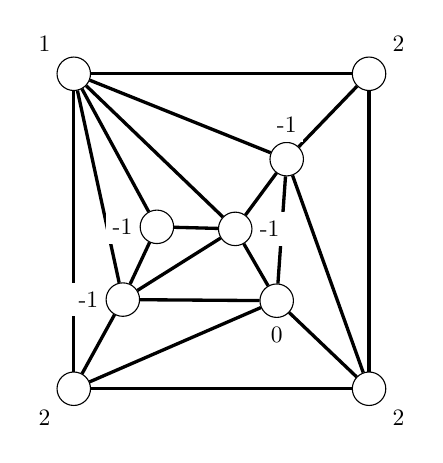
\begin{tikzpicture}
        \node (v0) [label=above left:{1}] at (-1.875000cm, 2.000000cm) {
};
        \node (v1) [label=above right:{2}] at (1.875000cm, 2.000000cm) {};
        \node (v2) [label=below right:{2}] at (1.875000cm, -2.000000cm) {};
        \node (v3) [label=below left:{2}] at (-1.875000cm, -2.000000cm) {};
        \node (v4) [label=above:{-1}] at (0.829462cm, 0.915182cm) {};
        \node (v5) [label=below:{0}] at (0.702189cm, -0.881858cm) {};
        \node (v6) [label=left:{-1}] at (-1.251848cm, -0.867854cm) {};
        \node (v7) [label=left:{-1}] at (-0.819321cm, 0.056225cm) {};
        \node (v8) [label=right:{-1}] at (0.175438cm, 0.030180cm) {};
        \begin{pgfonlayer}{bg}
                \draw (v5) edge [very thick] (v6);
                \draw (v6) edge [very thick] (v8);
                \draw (v6) edge [very thick] (v7);
                \draw (v7) edge [very thick] (v8);
                \draw (v5) edge [very thick] (v8);
                \draw (v4) edge [very thick] (v8);
                \draw (v4) edge [very thick] (v5);
                \draw (v0) edge [very thick] (v3);
                \draw (v0) edge [very thick] (v6);
                \draw (v0) edge [very thick] (v7);
                \draw (v0) edge [very thick] (v8);
                \draw (v0) edge [very thick] (v4);
                \draw (v0) edge [very thick] (v1);
                \draw (v1) edge [very thick] (v4);
                \draw (v1) edge [very thick] (v2);
                \draw (v2) edge [very thick] (v4);
                \draw (v2) edge [very thick] (v5);
                \draw (v2) edge [very thick] (v3);
                \draw (v3) edge [very thick] (v5);
                \draw (v3) edge [very thick] (v6);
        \end{pgfonlayer}
\end{tikzpicture}
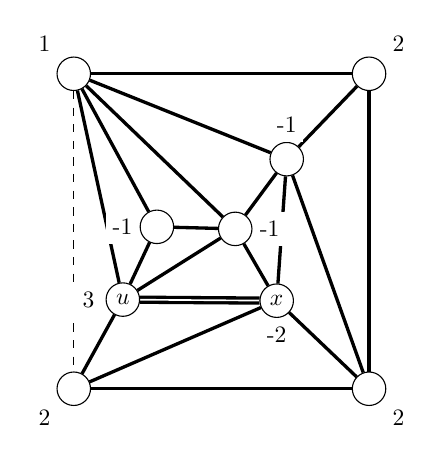
\begin{tikzpicture}
        \node (v0) [label=above left:{1}] at (-1.875000cm, 2.000000cm) {
};
        \node (v1) [label=above right:{2}] at (1.875000cm, 2.000000cm) {};
        \node (v2) [label=below right:{2}] at (1.875000cm, -2.000000cm) {};
        \node (v3) [label=below left:{2}] at (-1.875000cm, -2.000000cm) {};
        \node (v4) [label=above:{-1}] at (0.829462cm, 0.915182cm) {};
        \node (v5) [label=below:{-2}] at (0.702189cm, -0.881858cm) {$x$};
        \node (v6) [label=left:{3}] at (-1.251848cm, -0.867854cm) {$u$};
        \node (v7) [label=left:{-1}] at (-0.819321cm, 0.056225cm) {};
        \node (v8) [label=right:{-1}] at (0.175438cm, 0.030180cm) {};
        \begin{pgfonlayer}{bg}
                \draw (v5) edge [double, very thick] (v6);
                \draw (v6) edge [very thick] (v8);
                \draw (v6) edge [very thick] (v7);
                \draw (v7) edge [very thick] (v8);
                \draw (v5) edge [very thick] (v8);
                \draw (v4) edge [very thick] (v8);
                \draw (v4) edge [very thick] (v5);
                \draw (v0) edge [dashed] (v3);
                \draw (v0) edge [very thick] (v6);
                \draw (v0) edge [very thick] (v7);
                \draw (v0) edge [very thick] (v8);
                \draw (v0) edge [very thick] (v4);
                \draw (v0) edge [very thick] (v1);
                \draw (v1) edge [very thick] (v4);
                \draw (v1) edge [very thick] (v2);
                \draw (v2) edge [very thick] (v4);
                \draw (v2) edge [very thick] (v5);
                \draw (v2) edge [very thick] (v3);
                \draw (v3) edge [very thick] (v5);
                \draw (v3) edge [very thick] (v6);
        \end{pgfonlayer}
\end{tikzpicture}
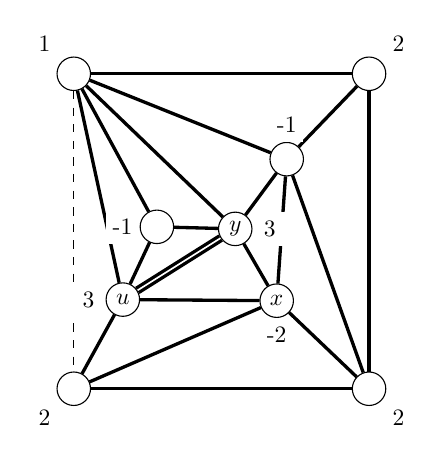
\begin{tikzpicture}
        \node (v0) [label=above left:{1}] at (-1.875000cm, 2.000000cm) {
};
        \node (v1) [label=above right:{2}] at (1.875000cm, 2.000000cm) {};
        \node (v2) [label=below right:{2}] at (1.875000cm, -2.000000cm) {};
        \node (v3) [label=below left:{2}] at (-1.875000cm, -2.000000cm) {};
        \node (v4) [label=above:{-1}] at (0.829462cm, 0.915182cm) {};
        \node (v5) [label=below:{-2}] at (0.702189cm, -0.881858cm) {$x$};
        \node (v6) [label=left:{3}] at (-1.251848cm, -0.867854cm) {$u$};
        \node (v7) [label=left:{-1}] at (-0.819321cm, 0.056225cm) {};
        \node (v8) [label=right:{3}] at (0.175438cm, 0.030180cm) {$y$};
        \begin{pgfonlayer}{bg}
                \draw (v6) edge [double, very thick] (v8);
                \draw (v6) edge [very thick] (v7);
                \draw (v7) edge [very thick] (v8);
                \draw (v5) edge [very thick] (v8);
                \draw (v5) edge [very thick] (v6);
                \draw (v4) edge [very thick] (v8);
                \draw (v4) edge [very thick] (v5);
                \draw (v0) edge [dashed] (v3);
                \draw (v0) edge [very thick] (v6);
                \draw (v0) edge [very thick] (v7);
                \draw (v0) edge [very thick] (v8);
                \draw (v0) edge [very thick] (v4);
                \draw (v0) edge [very thick] (v1);
                \draw (v1) edge [very thick] (v4);
                \draw (v1) edge [very thick] (v2);
                \draw (v2) edge [very thick] (v4);
                \draw (v2) edge [very thick] (v5);
                \draw (v2) edge [very thick] (v3);
                \draw (v3) edge [very thick] (v5);
                \draw (v3) edge [very thick] (v6);
        \end{pgfonlayer}
\end{tikzpicture}

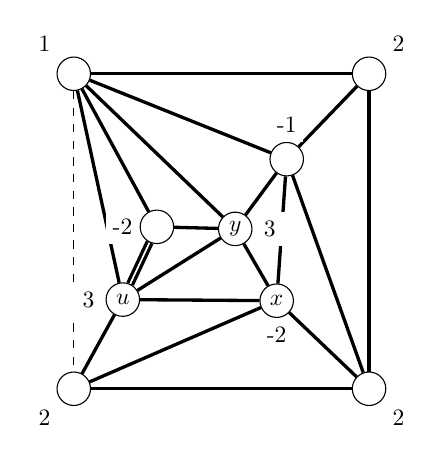
\begin{tikzpicture}
        \node (v0) [label=above left:{1}] at (-1.875000cm, 2.000000cm) {
};
        \node (v1) [label=above right:{2}] at (1.875000cm, 2.000000cm) {};
        \node (v2) [label=below right:{2}] at (1.875000cm, -2.000000cm) {};
        \node (v3) [label=below left:{2}] at (-1.875000cm, -2.000000cm) {};
        \node (v4) [label=above:{-1}] at (0.829462cm, 0.915182cm) {};
        \node (v5) [label=below:{-2}] at (0.702189cm, -0.881858cm) {$x$};
        \node (v6) [label=left:{3}] at (-1.251848cm, -0.867854cm) {$u$};
        \node (v7) [label=left:{-2}] at (-0.819321cm, 0.056225cm) {};
        \node (v8) [label=right:{3}] at (0.175438cm, 0.030180cm) {$y$};
        \begin{pgfonlayer}{bg}
                \draw (v0) edge [very thick] (v6);
                \draw (v5) edge [very thick] (v8);
                \draw (v5) edge [very thick] (v6);
                \draw (v4) edge [very thick] (v8);
                \draw (v4) edge [very thick] (v5);
                \draw (v7) edge [very thick] (v8);
                \draw (v0) edge [very thick] (v7);
                \draw (v0) edge [very thick] (v8);
                \draw (v0) edge [very thick] (v4);
                \draw (v0) edge [very thick] (v1);
                \draw (v1) edge [very thick] (v4);
                \draw (v1) edge [very thick] (v2);
                \draw (v2) edge [very thick] (v4);
                \draw (v2) edge [very thick] (v5);
                \draw (v2) edge [very thick] (v3);
                \draw (v3) edge [very thick] (v5);
                \draw (v3) edge [very thick] (v6);
                \draw (v6) edge [very thick] (v8);
                \draw (v6) edge [double, very thick] (v7);
                \draw (v0) edge [dashed] (v3);
        \end{pgfonlayer}
\end{tikzpicture}
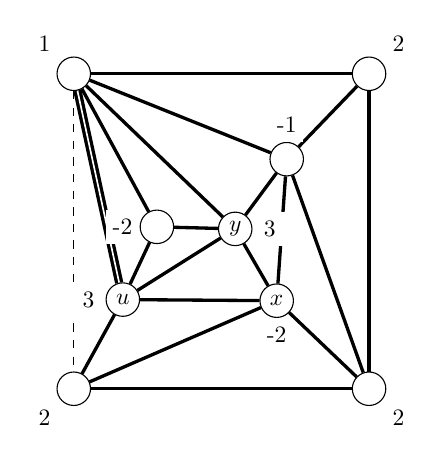
\begin{tikzpicture}
        \node (v0) [label=above left:{1}] at (-1.875000cm, 2.000000cm) {
};
        \node (v1) [label=above right:{2}] at (1.875000cm, 2.000000cm) {};
        \node (v2) [label=below right:{2}] at (1.875000cm, -2.000000cm) {};
        \node (v3) [label=below left:{2}] at (-1.875000cm, -2.000000cm) {};
        \node (v4) [label=above:{-1}] at (0.829462cm, 0.915182cm) {};
        \node (v5) [label=below:{-2}] at (0.702189cm, -0.881858cm) {$x$};
        \node (v6) [label=left:{3}] at (-1.251848cm, -0.867854cm) {$u$};
        \node (v7) [label=left:{-2}] at (-0.819321cm, 0.056225cm) {};
        \node (v8) [label=right:{3}] at (0.175438cm, 0.030180cm) {$y$};
        \begin{pgfonlayer}{bg}
                \draw (v0) edge [double, very thick] (v6);
                \draw (v5) edge [very thick] (v8);
                \draw (v5) edge [very thick] (v6);
                \draw (v4) edge [very thick] (v8);
                \draw (v4) edge [very thick] (v5);
                \draw (v7) edge [very thick] (v8);
                \draw (v0) edge [very thick] (v7);
                \draw (v0) edge [very thick] (v8);
                \draw (v0) edge [very thick] (v4);
                \draw (v0) edge [very thick] (v1);
                \draw (v1) edge [very thick] (v4);
                \draw (v1) edge [very thick] (v2);
                \draw (v2) edge [very thick] (v4);
                \draw (v2) edge [very thick] (v5);
                \draw (v2) edge [very thick] (v3);
                \draw (v3) edge [very thick] (v5);
                \draw (v3) edge [very thick] (v6);
                \draw (v6) edge [very thick] (v8);
                \draw (v6) edge [very thick] (v7);
                \draw (v0) edge [dashed] (v3);
        \end{pgfonlayer}
\end{tikzpicture}
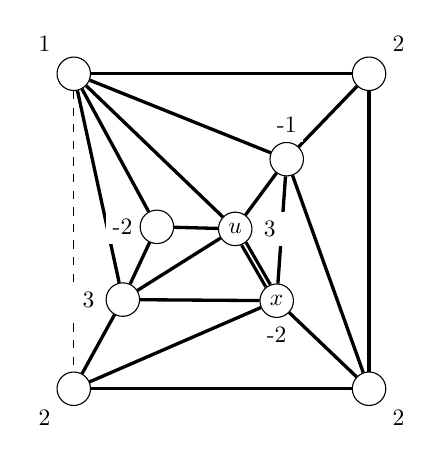
\begin{tikzpicture}
        \node (v0) [label=above left:{1}] at (-1.875000cm, 2.000000cm) {
};
        \node (v1) [label=above right:{2}] at (1.875000cm, 2.000000cm) {};
        \node (v2) [label=below right:{2}] at (1.875000cm, -2.000000cm) {};
        \node (v3) [label=below left:{2}] at (-1.875000cm, -2.000000cm) {};
        \node (v4) [label=above:{-1}] at (0.829462cm, 0.915182cm) {};
        \node (v5) [label=below:{-2}] at (0.702189cm, -0.881858cm) {$x$};
        \node (v6) [label=left:{3}] at (-1.251848cm, -0.867854cm) {};
        \node (v7) [label=left:{-2}] at (-0.819321cm, 0.056225cm) {};
        \node (v8) [label=right:{3}] at (0.175438cm, 0.030180cm) {$u$};
        \begin{pgfonlayer}{bg}
                \draw (v5) edge [double, very thick] (v8);
                \draw (v4) edge [very thick] (v8);
                \draw (v4) edge [very thick] (v5);
                \draw (v7) edge [very thick] (v8);
                \draw (v5) edge [very thick] (v6);
                \draw (v0) edge [very thick] (v6);
                \draw (v0) edge [very thick] (v7);
                \draw (v0) edge [very thick] (v8);
                \draw (v0) edge [very thick] (v4);
                \draw (v0) edge [very thick] (v1);
                \draw (v1) edge [very thick] (v4);
                \draw (v1) edge [very thick] (v2);
                \draw (v2) edge [very thick] (v4);
                \draw (v2) edge [very thick] (v5);
                \draw (v2) edge [very thick] (v3);
                \draw (v3) edge [very thick] (v5);
                \draw (v3) edge [very thick] (v6);
                \draw (v6) edge [very thick] (v8);
                \draw (v6) edge [very thick] (v7);
                \draw (v0) edge [dashed] (v3);
        \end{pgfonlayer}
\end{tikzpicture}

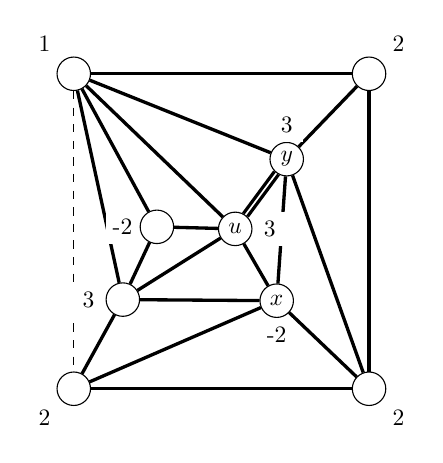
\begin{tikzpicture}
        \node (v0) [label=above left:{1}] at (-1.875000cm, 2.000000cm) {
};
        \node (v1) [label=above right:{2}] at (1.875000cm, 2.000000cm) {};
        \node (v2) [label=below right:{2}] at (1.875000cm, -2.000000cm) {};
        \node (v3) [label=below left:{2}] at (-1.875000cm, -2.000000cm) {};
        \node (v4) [label=above:{3}] at (0.829462cm, 0.915182cm) {$y$};
        \node (v5) [label=below:{-2}] at (0.702189cm, -0.881858cm) {$x$};
        \node (v6) [label=left:{3}] at (-1.251848cm, -0.867854cm) {};
        \node (v7) [label=left:{-2}] at (-0.819321cm, 0.056225cm) {};
        \node (v8) [label=right:{3}] at (0.175438cm, 0.030180cm) {$u$};
        \begin{pgfonlayer}{bg}
                \draw (v4) edge [double, very thick] (v8);
                \draw (v7) edge [very thick] (v8);
                \draw (v5) edge [very thick] (v8);
                \draw (v5) edge [very thick] (v6);
                \draw (v4) edge [very thick] (v5);
                \draw (v0) edge [very thick] (v6);
                \draw (v0) edge [very thick] (v7);
                \draw (v0) edge [very thick] (v8);
                \draw (v0) edge [very thick] (v4);
                \draw (v0) edge [very thick] (v1);
                \draw (v1) edge [very thick] (v4);
                \draw (v1) edge [very thick] (v2);
                \draw (v2) edge [very thick] (v4);
                \draw (v2) edge [very thick] (v5);
                \draw (v2) edge [very thick] (v3);
                \draw (v3) edge [very thick] (v5);
                \draw (v3) edge [very thick] (v6);
                \draw (v6) edge [very thick] (v8);
                \draw (v6) edge [very thick] (v7);
                \draw (v0) edge [dashed] (v3);
        \end{pgfonlayer}
\end{tikzpicture}
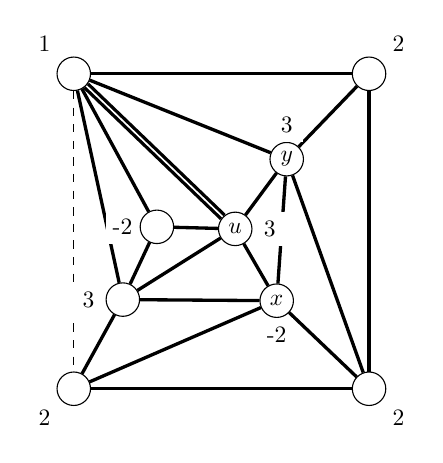
\begin{tikzpicture}
        \node (v0) [label=above left:{1}] at (-1.875000cm, 2.000000cm) {
};
        \node (v1) [label=above right:{2}] at (1.875000cm, 2.000000cm) {};
        \node (v2) [label=below right:{2}] at (1.875000cm, -2.000000cm) {};
        \node (v3) [label=below left:{2}] at (-1.875000cm, -2.000000cm) {};
        \node (v4) [label=above:{3}] at (0.829462cm, 0.915182cm) {$y$};
        \node (v5) [label=below:{-2}] at (0.702189cm, -0.881858cm) {$x$};
        \node (v6) [label=left:{3}] at (-1.251848cm, -0.867854cm) {};
        \node (v7) [label=left:{-2}] at (-0.819321cm, 0.056225cm) {};
        \node (v8) [label=right:{3}] at (0.175438cm, 0.030180cm) {$u$};
        \begin{pgfonlayer}{bg}
                \draw (v7) edge [very thick] (v8);
                \draw (v5) edge [very thick] (v8);
                \draw (v5) edge [very thick] (v6);
                \draw (v4) edge [very thick] (v8);
                \draw (v4) edge [very thick] (v5);
                \draw (v0) edge [very thick] (v6);
                \draw (v0) edge [very thick] (v7);
                \draw (v0) edge [double, very thick] (v8);
                \draw (v0) edge [very thick] (v4);
                \draw (v0) edge [very thick] (v1);
                \draw (v1) edge [very thick] (v4);
                \draw (v1) edge [very thick] (v2);
                \draw (v2) edge [very thick] (v4);
                \draw (v2) edge [very thick] (v5);
                \draw (v2) edge [very thick] (v3);
                \draw (v3) edge [very thick] (v5);
                \draw (v3) edge [very thick] (v6);
                \draw (v6) edge [very thick] (v8);
                \draw (v6) edge [very thick] (v7);
                \draw (v0) edge [dashed] (v3);
        \end{pgfonlayer}
\end{tikzpicture}
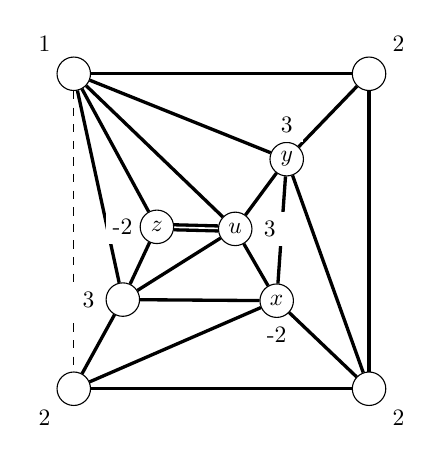
\begin{tikzpicture}
        \node (v0) [label=above left:{1}] at (-1.875000cm, 2.000000cm) {
};
        \node (v1) [label=above right:{2}] at (1.875000cm, 2.000000cm) {};
        \node (v2) [label=below right:{2}] at (1.875000cm, -2.000000cm) {};
        \node (v3) [label=below left:{2}] at (-1.875000cm, -2.000000cm) {};
        \node (v4) [label=above:{3}] at (0.829462cm, 0.915182cm) {$y$};
        \node (v5) [label=below:{-2}] at (0.702189cm, -0.881858cm) {$x$};
        \node (v6) [label=left:{3}] at (-1.251848cm, -0.867854cm) {};
        \node (v7) [label=left:{-2}] at (-0.819321cm, 0.056225cm) {$z$};
        \node (v8) [label=right:{3}] at (0.175438cm, 0.030180cm) {$u$};
        \begin{pgfonlayer}{bg}
                \draw (v6) edge [very thick] (v8);
                \draw (v5) edge [very thick] (v8);
                \draw (v5) edge [very thick] (v6);
                \draw (v4) edge [very thick] (v8);
                \draw (v4) edge [very thick] (v5);
                \draw (v0) edge [very thick] (v8);
                \draw (v0) edge [very thick] (v4);
                \draw (v0) edge [very thick] (v1);
                \draw (v1) edge [very thick] (v4);
                \draw (v1) edge [very thick] (v2);
                \draw (v2) edge [very thick] (v4);
                \draw (v2) edge [very thick] (v5);
                \draw (v2) edge [very thick] (v3);
                \draw (v3) edge [very thick] (v5);
                \draw (v3) edge [very thick] (v6);
                \draw (v0) edge [dashed] (v3);
                \draw (v0) edge [very thick](v6);
                \draw (v0) edge [very thick](v7);
                \draw (v6) edge [very thick](v7);
                \draw (v7) edge [double, very thick] (v8);
        \end{pgfonlayer}
\end{tikzpicture}

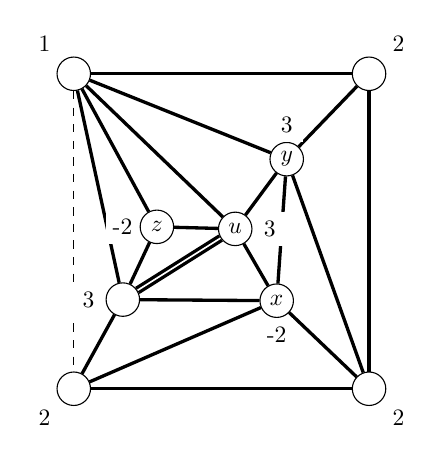
\begin{tikzpicture}
        \node (v0) [label=above left:{1}] at (-1.875000cm, 2.000000cm) {
};
        \node (v1) [label=above right:{2}] at (1.875000cm, 2.000000cm) {};
        \node (v2) [label=below right:{2}] at (1.875000cm, -2.000000cm) {};
        \node (v3) [label=below left:{2}] at (-1.875000cm, -2.000000cm) {};
        \node (v4) [label=above:{3}] at (0.829462cm, 0.915182cm) {$y$};
        \node (v5) [label=below:{-2}] at (0.702189cm, -0.881858cm) {$x$};
        \node (v6) [label=left:{3}] at (-1.251848cm, -0.867854cm) {};
        \node (v7) [label=left:{-2}] at (-0.819321cm, 0.056225cm) {$z$};
        \node (v8) [label=right:{3}] at (0.175438cm, 0.030180cm) {$u$};
        \begin{pgfonlayer}{bg}
                \draw (v6) edge [double, very thick] (v8);
                \draw (v5) edge [very thick] (v8);
                \draw (v5) edge [very thick] (v6);
                \draw (v4) edge [very thick] (v8);
                \draw (v4) edge [very thick] (v5);
                \draw (v0) edge [very thick] (v8);
                \draw (v0) edge [very thick] (v4);
                \draw (v0) edge [very thick] (v1);
                \draw (v1) edge [very thick] (v4);
                \draw (v1) edge [very thick] (v2);
                \draw (v2) edge [very thick] (v4);
                \draw (v2) edge [very thick] (v5);
                \draw (v2) edge [very thick] (v3);
                \draw (v3) edge [very thick] (v5);
                \draw (v3) edge [very thick] (v6);
                \draw (v0) edge [dashed] (v3);
                \draw (v0) [very thick] edge (v6);
                \draw (v0) [very thick] edge (v7);
                \draw (v6) [very thick] edge (v7);
                \draw (v7) [very thick] edge (v8);
        \end{pgfonlayer}
\end{tikzpicture}
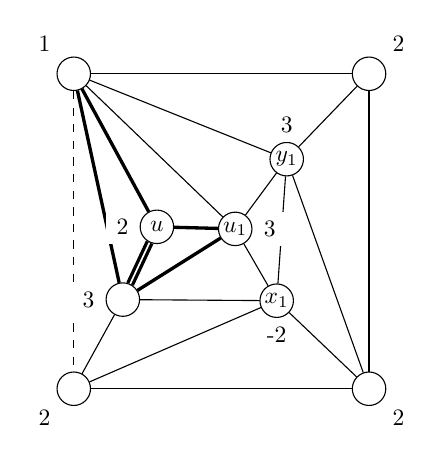
\begin{tikzpicture}
        \node (v0) [label=above left:{1}] at (-1.875000cm, 2.000000cm) {
};
        \node (v1) [label=above right:{2}] at (1.875000cm, 2.000000cm) {};
        \node (v2) [label=below right:{2}] at (1.875000cm, -2.000000cm) {};
        \node (v3) [label=below left:{2}] at (-1.875000cm, -2.000000cm) {};
        \node (v4) [label=above:{3}] at (0.829462cm, 0.915182cm) {$y_{1}$}
;
        \node (v5) [label=below:{-2}] at (0.702189cm, -0.881858cm) {$x_{1}$};
        \node (v6) [label=left:{3}] at (-1.251848cm, -0.867854cm) {};
        \node (v7) [label=left:{2}] at (-0.819321cm, 0.056225cm) {$u$};
        \node (v8) [label=right:{3}] at (0.175438cm, 0.030180cm) {$u_{1}$};
        \begin{pgfonlayer}{bg}
                \draw (v0) edge [very thick] (v7);
                \draw (v7) edge [very thick] (v8);
                \draw (v0) edge [very thick] (v6);
                \draw (v0) edge [thin] (v8);
                \draw (v6) edge [very thick] (v8);
                \draw (v6) edge [double, very thick] (v7);
                \draw (v5) edge [thin] (v8);
                \draw (v5) edge [thin] (v6);
                \draw (v4) edge [thin] (v8);
                \draw (v4) edge [thin] (v5);
                \draw (v0) edge [thin] (v4);
                \draw (v0) edge [thin] (v1);
                \draw (v1) edge [thin] (v4);
                \draw (v1) edge [thin] (v2);
                \draw (v2) edge [thin] (v4);
                \draw (v2) edge [thin] (v5);
                \draw (v2) edge [thin] (v3);
                \draw (v3) edge [thin] (v5);
                \draw (v3) edge [thin] (v6);
                \draw (v0) edge [dashed] (v3);
        \end{pgfonlayer}
\end{tikzpicture}
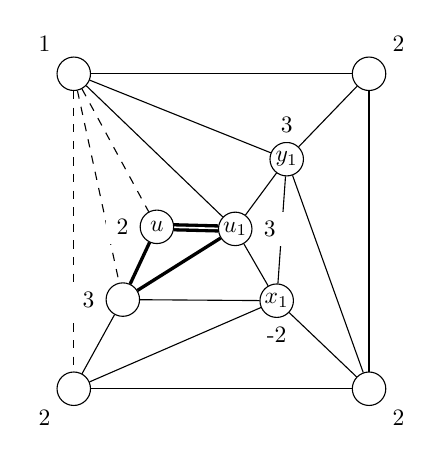
\begin{tikzpicture}
        \node (v0) [label=above left:{1}] at (-1.875000cm, 2.000000cm) {
};
        \node (v1) [label=above right:{2}] at (1.875000cm, 2.000000cm) {};
        \node (v2) [label=below right:{2}] at (1.875000cm, -2.000000cm) {};
        \node (v3) [label=below left:{2}] at (-1.875000cm, -2.000000cm) {};
        \node (v4) [label=above:{3}] at (0.829462cm, 0.915182cm) {$y_{1}$}
;
        \node (v5) [label=below:{-2}] at (0.702189cm, -0.881858cm) {$x_{1}$};
        \node (v6) [label=left:{3}] at (-1.251848cm, -0.867854cm) {};
        \node (v7) [label=left:{2}] at (-0.819321cm, 0.056225cm) {$u$};
        \node (v8) [label=right:{3}] at (0.175438cm, 0.030180cm) {$u_{1}$};
        \begin{pgfonlayer}{bg}
                \draw (v7) edge [double, very thick] (v8);
                \draw (v5) edge [thin] (v8);
                \draw (v5) edge [thin] (v6);
                \draw (v4) edge [thin] (v8);
                \draw (v4) edge [thin] (v5);
                \draw (v0) edge [thin] (v8);
                \draw (v0) edge [thin] (v4);
                \draw (v0) edge [thin] (v1);
                \draw (v1) edge [thin] (v4);
                \draw (v1) edge [thin] (v2);
                \draw (v2) edge [thin] (v4);
                \draw (v2) edge [thin] (v5);
                \draw (v2) edge [thin] (v3);
                \draw (v3) edge [thin] (v5);
                \draw (v3) edge [thin] (v6);
                \draw (v6) edge [very thick] (v8);
                \draw (v0) edge [dashed] (v3);
                \draw (v0) edge [dashed] (v6);
                \draw (v0) edge [dashed] (v7);
                \draw (v6) edge [very thick] (v7);
        \end{pgfonlayer}
\end{tikzpicture}
\caption{An example of Algorithm~\ref{A:poh_linear}. Each vertex $v\in G$ is
labelled with $c[v]$ if $c[v]>0$, and labelled with $-S[v]$ otherwise.}
\label{F:poh_example}
\end{center}
\end{figure}

\begin{figure}
\begin{center}
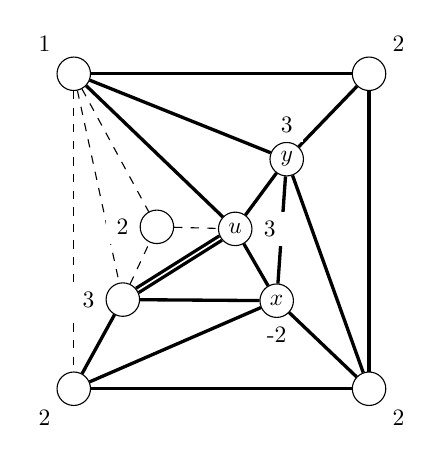
\begin{tikzpicture}
        \node (v0) [label=above left:{1}] at (-1.875000cm, 2.000000cm) {
};
        \node (v1) [label=above right:{2}] at (1.875000cm, 2.000000cm) {};
        \node (v2) [label=below right:{2}] at (1.875000cm, -2.000000cm) {};
        \node (v3) [label=below left:{2}] at (-1.875000cm, -2.000000cm) {};
        \node (v4) [label=above:{3}] at (0.829462cm, 0.915182cm) {$y$};
        \node (v5) [label=below:{-2}] at (0.702189cm, -0.881858cm) {$x$};
        \node (v6) [label=left:{3}] at (-1.251848cm, -0.867854cm) {};
        \node (v7) [label=left:{2}] at (-0.819321cm, 0.056225cm) {};
        \node (v8) [label=right:{3}] at (0.175438cm, 0.030180cm) {$u$};
        \begin{pgfonlayer}{bg}
                \draw (v6) edge [double, very thick] (v8);
                \draw (v5) edge [very thick] (v8);
                \draw (v5) edge [very thick] (v6);
                \draw (v4) edge [very thick] (v8);
                \draw (v4) edge [very thick] (v5);
                \draw (v0) edge [very thick] (v8);
                \draw (v0) edge [very thick] (v4);
                \draw (v0) edge [very thick] (v1);
                \draw (v1) edge [very thick] (v4);
                \draw (v1) edge [very thick] (v2);
                \draw (v2) edge [very thick] (v4);
                \draw (v2) edge [very thick] (v5);
                \draw (v2) edge [very thick] (v3);
                \draw (v3) edge [very thick] (v5);
                \draw (v3) edge [very thick] (v6);
                \draw (v0) edge [dashed] (v3);
                \draw (v0) edge [dashed] (v6);
                \draw (v0) edge [dashed] (v7);
                \draw (v6) edge [dashed] (v7);
                \draw (v7) edge [dashed] (v8);
        \end{pgfonlayer}
\end{tikzpicture}
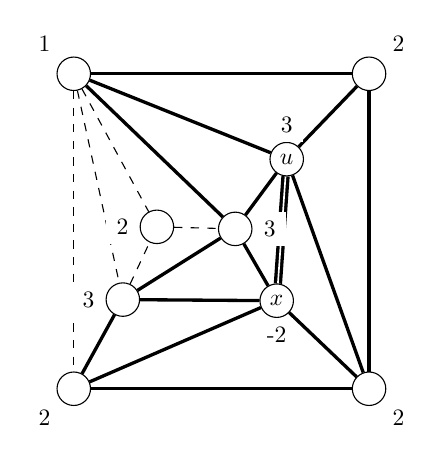
\begin{tikzpicture}
        \node (v0) [label=above left:{1}] at (-1.875000cm, 2.000000cm) {
};
        \node (v1) [label=above right:{2}] at (1.875000cm, 2.000000cm) {};
        \node (v2) [label=below right:{2}] at (1.875000cm, -2.000000cm) {};
        \node (v3) [label=below left:{2}] at (-1.875000cm, -2.000000cm) {};
        \node (v4) [label=above:{3}] at (0.829462cm, 0.915182cm) {$u$};
        \node (v5) [label=below:{-2}] at (0.702189cm, -0.881858cm) {$x$};
        \node (v6) [label=left:{3}] at (-1.251848cm, -0.867854cm) {};
        \node (v7) [label=left:{2}] at (-0.819321cm, 0.056225cm) {};
        \node (v8) [label=right:{3}] at (0.175438cm, 0.030180cm) {};
        \begin{pgfonlayer}{bg}
                \draw (v4) edge [double, very thick] (v5);
                \draw (v4) edge [very thick] (v8);
                \draw (v5) edge [very thick] (v8);
                \draw (v5) edge [very thick] (v6);
                \draw (v0) edge [very thick] (v8);
                \draw (v0) edge [very thick] (v4);
                \draw (v0) edge [very thick] (v1);
                \draw (v1) edge [very thick] (v4);
                \draw (v1) edge [very thick] (v2);
                \draw (v2) edge [very thick] (v4);
                \draw (v2) edge [very thick] (v5);
                \draw (v2) edge [very thick] (v3);
                \draw (v3) edge [very thick] (v5);
                \draw (v3) edge [very thick] (v6);
                \draw (v6) edge [very thick] (v8);
                \draw (v0) edge [dashed] (v3);
                \draw (v0) edge [dashed] (v6);
                \draw (v0) edge [dashed] (v7);
                \draw (v6) edge [dashed] (v7);
                \draw (v7) edge [dashed] (v8);
        \end{pgfonlayer}
\end{tikzpicture}
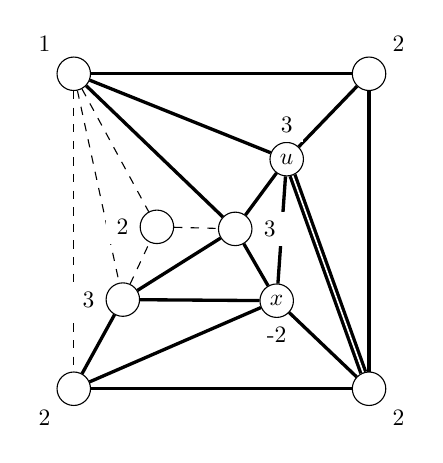
\begin{tikzpicture}
        \node (v0) [label=above left:{1}] at (-1.875000cm, 2.000000cm) {
};
        \node (v1) [label=above right:{2}] at (1.875000cm, 2.000000cm) {};
        \node (v2) [label=below right:{2}] at (1.875000cm, -2.000000cm) {};
        \node (v3) [label=below left:{2}] at (-1.875000cm, -2.000000cm) {};
        \node (v4) [label=above:{3}] at (0.829462cm, 0.915182cm) {$u$};
        \node (v5) [label=below:{-2}] at (0.702189cm, -0.881858cm) {$x$};
        \node (v6) [label=left:{3}] at (-1.251848cm, -0.867854cm) {};
        \node (v7) [label=left:{2}] at (-0.819321cm, 0.056225cm) {};
        \node (v8) [label=right:{3}] at (0.175438cm, 0.030180cm) {};
        \begin{pgfonlayer}{bg}
                \draw (v4) edge [very thick] (v5);
                \draw (v4) edge [very thick] (v8);
                \draw (v5) edge [very thick] (v8);
                \draw (v5) edge [very thick] (v6);
                \draw (v0) edge [very thick] (v8);
                \draw (v0) edge [very thick] (v4);
                \draw (v0) edge [very thick] (v1);
                \draw (v1) edge [very thick] (v4);
                \draw (v1) edge [very thick] (v2);
                \draw (v2) edge [double, very thick] (v4);
                \draw (v2) edge [very thick] (v5);
                \draw (v2) edge [very thick] (v3);
                \draw (v3) edge [very thick] (v5);
                \draw (v3) edge [very thick] (v6);
                \draw (v6) edge [very thick] (v8);
                \draw (v0) edge [dashed] (v3);
                \draw (v0) edge [dashed] (v6);
                \draw (v0) edge [dashed] (v7);
                \draw (v6) edge [dashed] (v7);
                \draw (v7) edge [dashed] (v8);
        \end{pgfonlayer}
\end{tikzpicture}

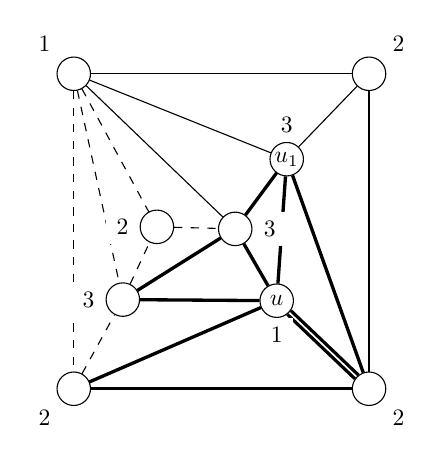
\begin{tikzpicture}
        \node (v0) [label=above left:{1}] at (-1.875000cm, 2.000000cm) {
};
        \node (v1) [label=above right:{2}] at (1.875000cm, 2.000000cm) {};
        \node (v2) [label=below right:{2}] at (1.875000cm, -2.000000cm) {};
        \node (v3) [label=below left:{2}] at (-1.875000cm, -2.000000cm) {};
        \node (v4) [label=above:{3}] at (0.829462cm, 0.915182cm) {$u_{1}$}
;
        \node (v5) [label=below:{1}] at (0.702189cm, -0.881858cm) {$u$};
        \node (v6) [label=left:{3}] at (-1.251848cm, -0.867854cm) {};
        \node (v7) [label=left:{2}] at (-0.819321cm, 0.056225cm) {};
        \node (v8) [label=right:{3}] at (0.175438cm, 0.030180cm) {};
        \begin{pgfonlayer}{bg}
                \draw (v3) edge [very thick] (v5);
                \draw (v5) edge [very thick] (v8);
                \draw (v5) edge [very thick] (v6);
                \draw (v2) edge [very thick] (v4);
                \draw (v2) edge [double, very thick] (v5);
                \draw (v2) edge [very thick] (v3);
                \draw (v3) edge [dashed] (v6);
                \draw (v4) edge [very thick] (v8);
                \draw (v4) edge [very thick] (v5);
                \draw (v6) edge [very thick] (v8);
                \draw (v0) edge [thin] (v8);
                \draw (v0) edge [thin] (v4);
                \draw (v0) edge [thin] (v1);
                \draw (v1) edge [thin] (v4);
                \draw (v1) edge [thin] (v2);
                \draw (v0) edge [dashed] (v3);
                \draw (v0) edge [dashed] (v6);
                \draw (v0) edge [dashed] (v7);
                \draw (v6) edge [dashed] (v7);
                \draw (v7) edge [dashed] (v8);
        \end{pgfonlayer}
\end{tikzpicture}
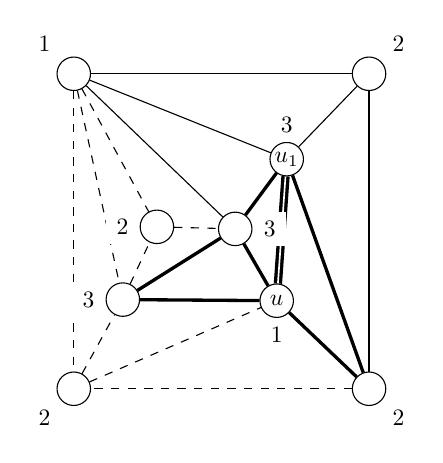
\begin{tikzpicture}
        \node (v0) [label=above left:{1}] at (-1.875000cm, 2.000000cm) {
};
        \node (v1) [label=above right:{2}] at (1.875000cm, 2.000000cm) {};
        \node (v2) [label=below right:{2}] at (1.875000cm, -2.000000cm) {};
        \node (v3) [label=below left:{2}] at (-1.875000cm, -2.000000cm) {};
        \node (v4) [label=above:{3}] at (0.829462cm, 0.915182cm) {$u_{1}$}
;
        \node (v5) [label=below:{1}] at (0.702189cm, -0.881858cm) {$u$};
        \node (v6) [label=left:{3}] at (-1.251848cm, -0.867854cm) {};
        \node (v7) [label=left:{2}] at (-0.819321cm, 0.056225cm) {};
        \node (v8) [label=right:{3}] at (0.175438cm, 0.030180cm) {};
        \begin{pgfonlayer}{bg}
                \draw (v3) edge [dashed] (v5);
                \draw (v5) edge [very thick] (v8);
                \draw (v5) edge [very thick] (v6);
                \draw (v2) edge [very thick] (v4);
                \draw (v2) edge [very thick] (v5);
                \draw (v2) edge [dashed] (v3);
                \draw (v3) edge [dashed] (v6);
                \draw (v4) edge [very thick] (v8);
                \draw (v4) edge [double, very thick] (v5);
                \draw (v6) edge [very thick] (v8);
                \draw (v0) edge [thin] (v8);
                \draw (v0) edge [thin] (v4);
                \draw (v0) edge [thin] (v1);
                \draw (v1) edge [thin] (v4);
                \draw (v1) edge [thin] (v2);
                \draw (v0) edge [dashed] (v3);
                \draw (v0) edge [dashed] (v6);
                \draw (v0) edge [dashed] (v7);
                \draw (v6) edge [dashed] (v7);
                \draw (v7) edge [dashed] (v8);
        \end{pgfonlayer}
\end{tikzpicture}
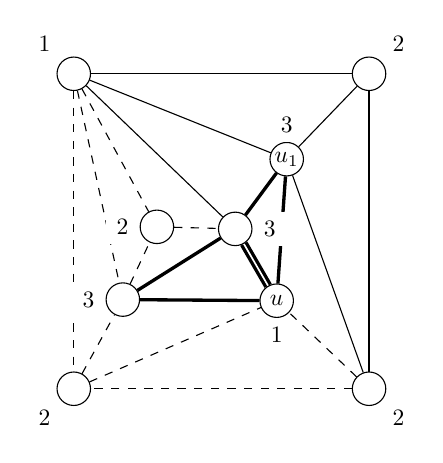
\begin{tikzpicture}
        \node (v0) [label=above left:{1}] at (-1.875000cm, 2.000000cm) {
};
        \node (v1) [label=above right:{2}] at (1.875000cm, 2.000000cm) {};
        \node (v2) [label=below right:{2}] at (1.875000cm, -2.000000cm) {};
        \node (v3) [label=below left:{2}] at (-1.875000cm, -2.000000cm) {};
        \node (v4) [label=above:{3}] at (0.829462cm, 0.915182cm) {$u_{1}$}
;
        \node (v5) [label=below:{1}] at (0.702189cm, -0.881858cm) {$u$};
        \node (v6) [label=left:{3}] at (-1.251848cm, -0.867854cm) {};
        \node (v7) [label=left:{2}] at (-0.819321cm, 0.056225cm) {};
        \node (v8) [label=right:{3}] at (0.175438cm, 0.030180cm) {};
        \begin{pgfonlayer}{bg}
                \draw (v3) edge [dashed] (v5);
                \draw (v5) edge [double, very thick] (v8);
                \draw (v5) edge [very thick] (v6);
                \draw (v2) edge [thin] (v4);
                \draw (v2) edge [dashed] (v5);
                \draw (v2) edge [dashed] (v3);
                \draw (v3) edge [dashed] (v6);
                \draw (v4) edge [very thick] (v8);
                \draw (v4) edge [very thick] (v5);
                \draw (v6) edge [very thick] (v8);
                \draw (v0) edge [thin] (v8);
                \draw (v0) edge [thin] (v4);
                \draw (v0) edge [thin] (v1);
                \draw (v1) edge [thin] (v4);
                \draw (v1) edge [thin] (v2);
                \draw (v0) edge [dashed] (v3);
                \draw (v0) edge [dashed] (v6);
                \draw (v0) edge [dashed] (v7);
                \draw (v6) edge [dashed] (v7);
                \draw (v7) edge [dashed] (v8);
        \end{pgfonlayer}
\end{tikzpicture}

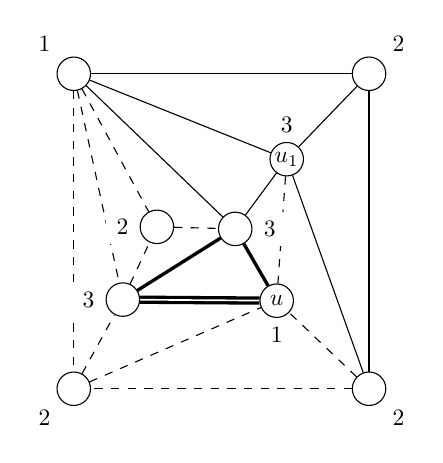
\begin{tikzpicture}
        \node (v0) [label=above left:{1}] at (-1.875000cm, 2.000000cm) {
};
        \node (v1) [label=above right:{2}] at (1.875000cm, 2.000000cm) {};
        \node (v2) [label=below right:{2}] at (1.875000cm, -2.000000cm) {};
        \node (v3) [label=below left:{2}] at (-1.875000cm, -2.000000cm) {};
        \node (v4) [label=above:{3}] at (0.829462cm, 0.915182cm) {$u_{1}$}
;
        \node (v5) [label=below:{1}] at (0.702189cm, -0.881858cm) {$u$};
        \node (v6) [label=left:{3}] at (-1.251848cm, -0.867854cm) {};
        \node (v7) [label=left:{2}] at (-0.819321cm, 0.056225cm) {};
        \node (v8) [label=right:{3}] at (0.175438cm, 0.030180cm) {};
        \begin{pgfonlayer}{bg}
                \draw (v5) edge [double, very thick] (v6);
                \draw (v4) edge [thin] (v8);
                \draw (v0) edge [thin] (v8);
                \draw (v0) edge [thin] (v4);
                \draw (v0) edge [thin] (v1);
                \draw (v1) edge [thin] (v4);
                \draw (v1) edge [thin] (v2);
                \draw (v0) edge [dashed] (v3);
                \draw (v0) edge [dashed] (v6);
                \draw (v0) edge [dashed] (v7);
                \draw (v2) [thin] edge (v4);
                \draw (v2) edge [dashed] (v5);
                \draw (v2) edge [dashed] (v3);
                \draw (v3) edge [dashed] (v5);
                \draw (v3) edge [dashed] (v6);
                \draw (v4) edge [dashed] (v5);
                \draw (v5) edge [very thick] (v8);
                \draw (v6) edge [very thick] (v8);
                \draw (v6) edge [dashed] (v7);
                \draw (v7) edge [dashed] (v8);
        \end{pgfonlayer}
\end{tikzpicture}
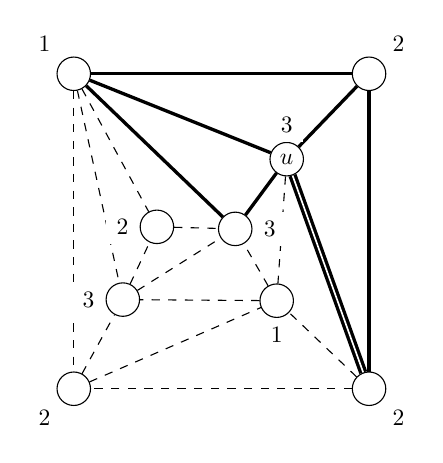
\begin{tikzpicture}
        \node (v0) [label=above left:{1}] at (-1.875000cm, 2.000000cm) {
};
        \node (v1) [label=above right:{2}] at (1.875000cm, 2.000000cm) {};
        \node (v2) [label=below right:{2}] at (1.875000cm, -2.000000cm) {};
        \node (v3) [label=below left:{2}] at (-1.875000cm, -2.000000cm) {};
        \node (v4) [label=above:{3}] at (0.829462cm, 0.915182cm) {$u$};
        \node (v5) [label=below:{1}] at (0.702189cm, -0.881858cm) {};
        \node (v6) [label=left:{3}] at (-1.251848cm, -0.867854cm) {};
        \node (v7) [label=left:{2}] at (-0.819321cm, 0.056225cm) {};
        \node (v8) [label=right:{3}] at (0.175438cm, 0.030180cm) {};
        \begin{pgfonlayer}{bg}
                \draw (v2) edge [double, very thick] (v4);
                \draw (v4) edge [very thick] (v8);
                \draw (v0) edge [very thick] (v8);
                \draw (v0) edge [very thick] (v4);
                \draw (v0) edge [very thick] (v1);
                \draw (v1) edge [very thick] (v4);
                \draw (v1) edge [very thick] (v2);
                \draw (v0) edge [dashed] (v3);
                \draw (v0) edge [dashed] (v6);
                \draw (v0) edge [dashed] (v7);
                \draw (v2) edge [dashed] (v5);
                \draw (v2) edge [dashed] (v3);
                \draw (v3) edge [dashed] (v5);
                \draw (v3) edge [dashed] (v6);
                \draw (v4) edge [dashed] (v5);
                \draw (v5) edge [dashed] (v8);
                \draw (v5) edge [dashed] (v6);
                \draw (v6) edge [dashed] (v8);
                \draw (v6) edge [dashed] (v7);
                \draw (v7) edge [dashed] (v8);
        \end{pgfonlayer}
\end{tikzpicture}
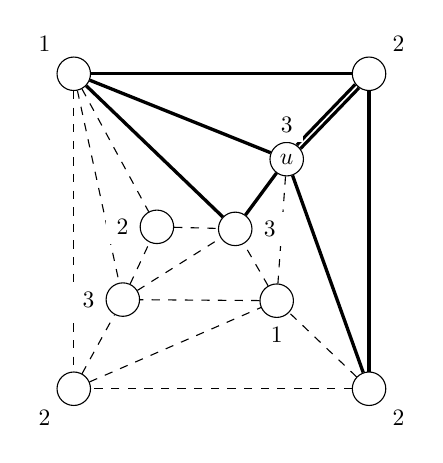
\begin{tikzpicture}
        \node (v0) [label=above left:{1}] at (-1.875000cm, 2.000000cm) {
};
        \node (v1) [label=above right:{2}] at (1.875000cm, 2.000000cm) {};
        \node (v2) [label=below right:{2}] at (1.875000cm, -2.000000cm) {};
        \node (v3) [label=below left:{2}] at (-1.875000cm, -2.000000cm) {};
        \node (v4) [label=above:{3}] at (0.829462cm, 0.915182cm) {$u$};
        \node (v5) [label=below:{1}] at (0.702189cm, -0.881858cm) {};
        \node (v6) [label=left:{3}] at (-1.251848cm, -0.867854cm) {};
        \node (v7) [label=left:{2}] at (-0.819321cm, 0.056225cm) {};
        \node (v8) [label=right:{3}] at (0.175438cm, 0.030180cm) {};
        \begin{pgfonlayer}{bg}
                \draw (v2) edge [very thick] (v4);
                \draw (v4) edge [very thick] (v8);
                \draw (v0) edge [very thick] (v8);
                \draw (v0) edge [very thick] (v4);
                \draw (v0) edge [very thick] (v1);
                \draw (v1) edge [double, very thick] (v4);
                \draw (v1) edge [very thick] (v2);
                \draw (v0) edge [dashed] (v3);
                \draw (v0) edge [dashed] (v6);
                \draw (v0) edge [dashed] (v7);
                \draw (v2) edge [dashed] (v5);
                \draw (v2) edge [dashed] (v3);
                \draw (v3) edge [dashed] (v5);
                \draw (v3) edge [dashed] (v6);
                \draw (v4) edge [dashed] (v5);
                \draw (v5) edge [dashed] (v8);
                \draw (v5) edge [dashed] (v6);
                \draw (v6) edge [dashed] (v8);
                \draw (v6) edge [dashed] (v7);
                \draw (v7) edge [dashed] (v8);
        \end{pgfonlayer}
\end{tikzpicture}

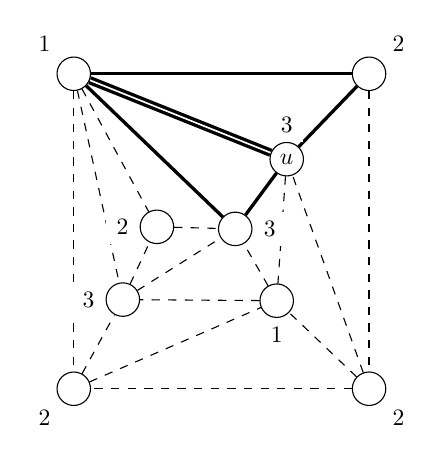
\begin{tikzpicture}
        \node (v0) [label=above left:{1}] at (-1.875000cm, 2.000000cm) {
};
        \node (v1) [label=above right:{2}] at (1.875000cm, 2.000000cm) {};
        \node (v2) [label=below right:{2}] at (1.875000cm, -2.000000cm) {};
        \node (v3) [label=below left:{2}] at (-1.875000cm, -2.000000cm) {};
        \node (v4) [label=above:{3}] at (0.829462cm, 0.915182cm) {$u$};
        \node (v5) [label=below:{1}] at (0.702189cm, -0.881858cm) {};
        \node (v6) [label=left:{3}] at (-1.251848cm, -0.867854cm) {};
        \node (v7) [label=left:{2}] at (-0.819321cm, 0.056225cm) {};
        \node (v8) [label=right:{3}] at (0.175438cm, 0.030180cm) {};
        \begin{pgfonlayer}{bg}
                \draw (v2) edge [dashed] (v4);
                \draw (v4) edge [very thick] (v8);
                \draw (v0) edge [very thick] (v8);
                \draw (v0) edge [double, very thick] (v4);
                \draw (v0) edge [very thick] (v1);
                \draw (v1) edge [very thick] (v4);
                \draw (v1) edge [dashed] (v2);
                \draw (v0) edge [dashed] (v3);
                \draw (v0) edge [dashed] (v6);
                \draw (v0) edge [dashed] (v7);
                \draw (v2) edge [dashed] (v5);
                \draw (v2) edge [dashed] (v3);
                \draw (v3) edge [dashed] (v5);
                \draw (v3) edge [dashed] (v6);
                \draw (v4) edge [dashed] (v5);
                \draw (v5) edge [dashed] (v8);
                \draw (v5) edge [dashed] (v6);
                \draw (v6) edge [dashed] (v8);
                \draw (v6) edge [dashed] (v7);
                \draw (v7) edge [dashed] (v8);
        \end{pgfonlayer}
\end{tikzpicture}
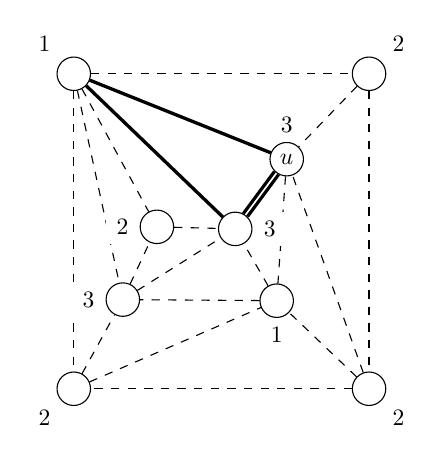
\begin{tikzpicture}
        \node (v0) [label=above left:{1}] at (-1.875000cm, 2.000000cm) {
};
        \node (v1) [label=above right:{2}] at (1.875000cm, 2.000000cm) {};
        \node (v2) [label=below right:{2}] at (1.875000cm, -2.000000cm) {};
        \node (v3) [label=below left:{2}] at (-1.875000cm, -2.000000cm) {};
        \node (v4) [label=above:{3}] at (0.829462cm, 0.915182cm) {$u$};
        \node (v5) [label=below:{1}] at (0.702189cm, -0.881858cm) {};
        \node (v6) [label=left:{3}] at (-1.251848cm, -0.867854cm) {};
        \node (v7) [label=left:{2}] at (-0.819321cm, 0.056225cm) {};
        \node (v8) [label=right:{3}] at (0.175438cm, 0.030180cm) {};
        \begin{pgfonlayer}{bg}
                \draw (v4) edge [double, very thick] (v8);
                \draw (v0) edge [dashed] (v3);
                \draw (v0) edge [dashed] (v6);
                \draw (v0) edge [dashed] (v7);
                \draw (v0) edge [very thick] (v8);
                \draw (v0) edge [very thick] (v4);
                \draw (v0) edge [dashed] (v1);
                \draw (v1) edge [dashed] (v4);
                \draw (v1) edge [dashed] (v2);
                \draw (v2) edge [dashed] (v4);
                \draw (v2) edge [dashed] (v5);
                \draw (v2) edge [dashed] (v3);
                \draw (v3) edge [dashed] (v5);
                \draw (v3) edge [dashed] (v6);
                \draw (v4) edge [dashed] (v5);
                \draw (v5) edge [dashed] (v8);
                \draw (v5) edge [dashed] (v6);
                \draw (v6) edge [dashed] (v8);
                \draw (v6) edge [dashed] (v7);
                \draw (v7) edge [dashed] (v8);
        \end{pgfonlayer}
\end{tikzpicture}
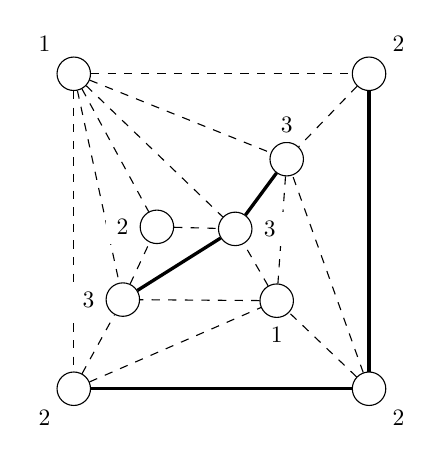
\begin{tikzpicture}
        \node (v0) [label=above left:{1}] at (-1.875000cm, 2.000000cm) {};
        \node (v1) [label=above right:{2}] at (1.875000cm, 2.000000cm) {};
        \node (v2) [label=below right:{2}] at (1.875000cm, -2.000000cm) {};
        \node (v3) [label=below left:{2}] at (-1.875000cm, -2.000000cm) {};
        \node (v4) [label=above:{3}] at (0.829462cm, 0.915182cm) {};
        \node (v5) [label=below:{1}] at (0.702189cm, -0.881858cm) {};
        \node (v6) [label=left:{3}] at (-1.251848cm, -0.867854cm) {};
        \node (v7) [label=left:{2}] at (-0.819321cm, 0.056225cm) {};
        \node (v8) [label=right:{3}] at (0.175438cm, 0.030180cm) {};
        \begin{pgfonlayer}{bg}
                \draw (v0) edge [dashed] (v1);
                \draw (v0) edge [dashed](v3);
                \draw (v0) edge [dashed](v6);
                \draw (v0) edge [dashed](v7);
                \draw (v0) edge [dashed](v8);
                \draw (v0) edge [dashed](v4);
                \draw (v1) edge [dashed](v4);
                \draw (v1) edge [very thick](v2);
                \draw (v2) edge [dashed](v4);
                \draw (v2) edge [dashed](v5);
                \draw (v2) edge [very thick](v3);
                \draw (v3) edge [dashed](v5);
                \draw (v3) edge [dashed](v6);
                \draw (v4) edge [very thick](v8);
                \draw (v4) edge [dashed](v5);
                \draw (v5) edge [dashed](v8);
                \draw (v5) edge [dashed](v6);
                \draw (v6) edge [very thick](v8);
                \draw (v6) edge [dashed](v7);
                \draw (v7) edge [dashed](v8);
        \end{pgfonlayer}
\end{tikzpicture}
\caption{An Algorithm~\ref{A:poh_linear} example, continued from
Figure~\ref{F:poh_example}.}
\label{F:poh_example_cont}
\end{center}
\end{figure}

While executing Algorithm~\ref{A:poh_linear} we iterate through
the adjacency list of each vertex $v\in G$ exactly twice: once to
orient $\text{Adj}[v]$
around a particular edge when $v$ is colored,
and once to examine each neighbor in $\text{Adj}[v]$ during Step~1.
Therefore the time complexity of the algorithm is
$\mathcal{O}(m)=\mathcal{O}(n)$. See Figure~\ref{F:poh_example} 
and Figure~\ref{F:poh_example_cont} for a concrete example of
Algorithm~\ref{A:poh_linear}.

Given a triangulated plane graph $G$ with adjacency list representation
$\text{Adj}$, we can set up the initial conditions for
Algorithm~\ref{A:poh_linear} as follows. First, create length $n$ integer
arrays for $c$ and $S$, initializing each entry to zero.
Let $C=v_1,v_2,v_3$ be the outer triangle of $G$,
labeled in clockwise order.
Color $c[v_1]\leftarrow 1$, then color $c[v_2]\leftarrow 2$ and
$c[v_3]\leftarrow 2$.
Iterate through $\text{Adj}[v_1]$ and mark $S[v]\leftarrow 1$ for each
neighbor $v$ of $v_1$.
Let $u$ be the vertex immediately counter-clockwise from $v_3$ in
$\text{Adj}[v_1]$. The vertex $u$ and the entry for $v_3$ in $\text{Adj}[u]$,
together with $\text{Adj}$, $c$, and $S$ form a valid input for
Algorithm~\ref{A:poh_linear}.

\section{Path List-Coloring}

In this section we describe a linear time algorithm to path color
plane graphs such that each vertex receives a color from a specified list.
Hartman showed that this is always possible when each vertex is given a
list of $3$ colors~\cite[Thm.~4.1]{Har1997}. Around the same
time \v{S}krekovski proved a
slightly weaker result using the same coloring
strategy~\cite[Thm.~2.2b]{Skr1999}.

The path list-coloring procedure discussed in this section is
based on the constructive proofs found in Hartman and
\v{S}krekovski's papers, but it ``localizes'' the logic to proceed through the
graph one edge at a time. The resulting algorithm
will produce different colorings in some situations.

A \defterm{list assignment} of a graph $G$ is
a function $L:V(G)\to P_{<\aleph_0}(\mathbb{N})$ assigning
a finite list of colors to each vertex. If $L$ is a list assignment of $G$,
an \defterm{$L$-coloring} of $G$ is a coloring function
$c:V(G)\to\mathbb{N}$ such that $c(v)\in L(v)$ for each $v\in V(G)$.

Given a graph $G$ and a coloring $c$ of $G$, for each $v\in G$ we
define $\text{deg}_c(v)$ to be the number of neighbors of $v$ that share a color
with $v$. Equivalently, $\text{deg}_c(v)$ is the degree of $v$ in the subgraph
of $G$ induced by the color class of $c(v)$.

Let $C$ be the outer face of a $2$-connected, weakly triangulated plane graph
$G$ and let $u,v\in C$ be vertices.
If $n(G)\ge3$, then $C$ is a cycle and we
define $C(u,v)$ to be the clockwise $u,v$-path
around $C$. If $n(G)<3$ then we define $C(u,v)=C$ if
$u\ne v$, and $C(u,u)=u$.

\begin{lemma}\label{L:hartman3}
Let $G$ be a $2$-connected, weakly triangulated plane graph with outer face
$C$. Let $x,y,z\in C$ be vertices (not necessarily distinct) such that
$z\in C(x,y)$. Let $L$ be a list assigment of $G$ such that
\begin{align*}
    |L(v)| &= 1 \text{ for } v\in\{x,y,z\},\\
    |L(v)| &\ge 2 \text{ for } v\in C-\{x,y,z\},\\
    |L(v)| &\ge 3 \text{ for } v\in G-C,
\end{align*}
and if $v\in C(x,z)-z$, then $L(v)\cap L(z)=\emptyset$.
There exists a path $L$-coloring of $G$ such that $\text{deg}_c(x)\le 1$,
$\text{deg}_c(y)\le 1$, and $\text{deg}_c(z)\le 1$. Moreover,
if $z=y$ or $C(z,y)=z,y$ and $L(z)\cap L(y)=\emptyset$,
then $\text{deg}_c(z)=0$.
\end{lemma}

\begin{proof}
Define $c(x)\in L(x)$, $c(y)\in L(y)$, and $c(z)\in L(z)$ to be the color in
each respective list.

Suppose that $m=|E(G)|\le 2$ and therefore $G=C$.
If $m=0$, then $n(G)=1$ and $x=y$ and $G$ is colored.
If $m=1$, then $n(G)= 2$. If $x\ne y$, then $C=x,y$ and $G$ is colored.
If $x=y$, then the remaining vertex
$v\in G-C(x,y)$ satisfies $|L(v)|\ge 2$. Choose $c(v)\in L(v)-\{c(x)\}$.

We proceed by induction on the number of edges $m=|E(G)|$. Let
$u_1,u_2,\ldots,u_k$ label the neighbors of $z$ in counter-clockwise
order such that $u_1$ is the vertex immediately counter-clockwise from $z$ around $C$
and $u_k$ is the vertex immediately clockwise from $z$ around $C$.

\begin{figure}[ht]
\begin{center}
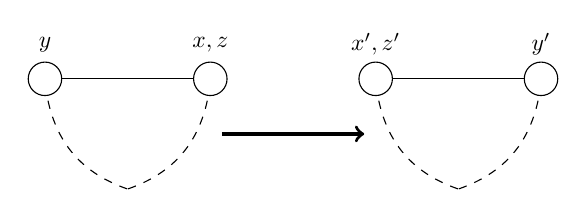
\begin{tikzpicture}[scale=1.4]
    %\node (ya) at (-3.5cm, 1.0cm) [label=above:${x',z'}$] {};
    %\node (xa) at (-2.0cm, 1.0cm) [label=above:${y'}$] {};
    %\node (bota) at (-2.75cm, 0.0cm) [draw=none, fill=none, minimum size=0mm] {};

    %\begin{pgfonlayer}{bg}
    %    \draw (xa) edge (ya);
    %    \draw (bota) edge [dashed, bend right] (xa);
    %    \draw (bota) edge [dashed, bend left] (ya);
    %\end{pgfonlayer}

    %\node (as) at (-0.1cm, 0.5cm) [draw=none, fill=none, minimum size=0mm] {};
    %\node (ae) at (-1.9cm, 0.5cm) [draw=none, fill=none, minimum size=0mm] {};

    %\draw (as) edge[->] node[above=0.2cm, shape=rectangle, draw=none,
    %    fill=white, text width=2.5cm]
    %        {if $c(x)=c(y)$}
    %    (ae);

    \node (y) at (0.0cm, 1.0cm) [label=above:${y}$] {};
    \node (x) at (1.5cm, 1.0cm) [label=above:${x,z}$] {};
    \node (bot) at (0.75cm, 0.0cm) [draw=none, fill=none, minimum size=0mm] {};

    \begin{pgfonlayer}{bg}
        \draw (x) edge (y);
        \draw (bot) edge [dashed, bend right] (x);
        \draw (bot) edge [dashed, bend left] (y);
    \end{pgfonlayer}

    \node (yb) at (3.0cm, 1.0cm) [label=above:${x',z'}$] {};
    \node (xb) at (4.5cm, 1.0cm) [label=above:${y'}$] {};
    \node (botb) at (3.75cm, 0.0cm) [draw=none, fill=none, minimum size=0mm] {};

    \node (bs) at (1.6cm, 0.5cm) [draw=none, fill=none, minimum size=0mm] {};
    \node (be) at (2.9cm, 0.5cm) [draw=none, fill=none, minimum size=0mm] {};

    \draw (bs) edge[very thick, ->]
        %node[above=0.2cm, shape=rectangle, draw=none, fill=white,
        %    text width=2.5cm]
        %    {if $c(x)\ne c(y)$}
        (be);

    \begin{pgfonlayer}{bg}
        \draw (xb) edge (yb);
        \draw (botb) edge [dashed, bend right] (xb);
        \draw (botb) edge [dashed, bend left] (yb);
    \end{pgfonlayer}
\end{tikzpicture}
$\qquad$
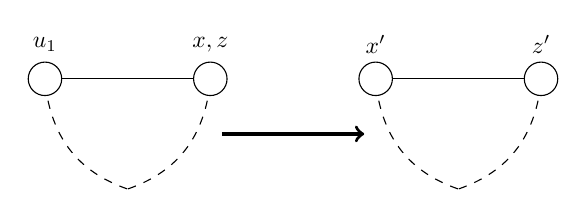
\begin{tikzpicture}[scale=1.4]
    \node (u1) at (0.0cm, 1.0cm) [label=above:${u_1}$] {};
    \node (x) at (1.5cm, 1.0cm) [label=above:${x,z}$] {};
    \node (bot) at (0.75cm, 0.0cm) [draw=none, fill=none, minimum size=0mm] {};

    \begin{pgfonlayer}{bg}
        \draw (x) edge (u1);
        \draw (bot) edge [dashed, bend right] (x);
        \draw (bot) edge [dashed, bend left] (u1);
    \end{pgfonlayer}

    \node (u1b) at (3.0cm, 1.0cm) [label=above:${x'}$] {};
    \node (xb) at (4.5cm, 1.0cm) [label=above:${z'}$] {};
    \node (botb) at (3.75cm, 0.0cm) [draw=none, fill=none, minimum size=0mm] {};

    \node (bs) at (1.6cm, 0.5cm) [draw=none, fill=none, minimum size=0mm] {};
    \node (be) at (2.9cm, 0.5cm) [draw=none, fill=none, minimum size=0mm] {};

    \draw (bs) edge[very thick, ->] (be);

    \begin{pgfonlayer}{bg}
        \draw (xb) edge (u1b);
        \draw (botb) edge [dashed, bend right] (xb);
        \draw (botb) edge [dashed, bend left] (u1b);
    \end{pgfonlayer}
\end{tikzpicture}
    \caption{The proof of Lemma~\ref{L:hartman3}, Case~1 (left) and Case~2 (right).}
\end{center}
\end{figure}

\textbf{Case 1.}
Suppose that $u_1=y$. Note that $z=x$ since $z\in C(x,y)$. Therefore
$V(C(z,y))=V(C)$ and $|V(C(z,y))|\ge 3$.
Apply the lemma with vertices re-labeled as $x'=y$, $y'=x$,
and $z'=y$ to find a path $L$-coloring $c$ of $G$.

\textbf{Case 2.}
Suppose that $u_1\ne y$ and $z=x$. Then $u_1\not\in\{x,y,z\}$
and $|L(u_1)|\ge 2$. Pick $c(u_1)\in L(u_1)-c(z)$. Define
$L'(u_1)=\{c(u_1)\}$ and $L'(v)=L(v)$ for each $v\in G-u_1$. Apply the
lemma with vertices re-labeled as $x'=u_1$, $y'=y$, and $z'=z$.

\textbf{Case 3.}
Suppose that $u_1\ne y$ and $z\ne x$. 
Our strategy will be to apply the inductive hypothesis to $G-zu_1$
with the embedding inherited from $G$.
Because $u_1\in C(x,z)$, it is guaranteed that $L(u_1)\cap L(z)=\emptyset$.
Thus any path $L$-coloring of $G-zu_1$ will also be a path $L$-coloring
of $G$.

\begin{figure}[ht]
\begin{center}
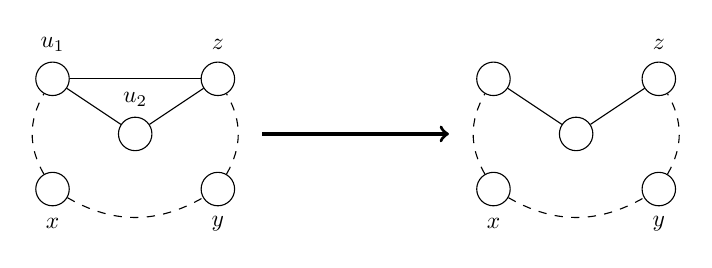
\begin{tikzpicture}[scale=1.4]
    \node (u1) at (0.0cm, 1.0cm) [label=above:${u_1}$] {};
    \node (v) at (0.75cm, 0.5cm) [label=above:${u_2}$] {};
    \node (z) at (1.5cm, 1.0cm) [label=above:${z}$] {};
    \node (x) at (0.0cm, 0.0cm) [label=below:${x}$] {};
    \node (y) at (1.5cm, 0.0cm) [label=below:${y}$] {};

    \begin{pgfonlayer}{bg}
        \draw (z) edge (u1);
        \draw (z) edge (v);
        \draw (u1) edge (v);
        \draw (y) edge [dashed, bend right] (z);
        \draw (x) edge [dashed, bend left] (u1);
        \draw (x) edge [dashed, bend right] (y);
    \end{pgfonlayer}

    \node (u1b) at (4.0cm, 1.0cm) {};
    \node (vb) at (4.75cm, 0.5cm) {};
    \node (zb) at (5.5cm, 1.0cm) [label=above:${z}$] {};
    \node (xb) at (4.0cm, 0.0cm) [label=below:${x}$] {};
    \node (yb) at (5.5cm, 0.0cm) [label=below:${y}$] {};

    \node (bs) at (1.9cm, 0.5cm) [draw=none, fill=none, minimum size=0mm] {};
    \node (be) at (3.6cm, 0.5cm) [draw=none, fill=none, minimum size=0mm] {};

    \draw (bs) edge[very thick, ->] (be);

    \begin{pgfonlayer}{bg}
        \draw (zb) edge (vb);
        \draw (u1b) edge (vb);
        \draw (yb) edge [dashed, bend right] (zb);
        \draw (xb) edge [dashed, bend left] (u1b);
        \draw (xb) edge [dashed, bend right] (yb);
    \end{pgfonlayer}
\end{tikzpicture}
\caption{The proof of Lemma~\ref{L:hartman3}, Case~3.1.}
\end{center}
\end{figure}

\textbf{Case 3.1.}
Suppose that $u_2\in G-C$. Define $L'(u_2)=L(u_2)-c(z)$ and
$L'(v)=L(v)$ for each $v\in G-u_2$. Note that $|L'(u_2)|\ge |L(v)|-1\ge 2$.
Let $C'$ be the outer face of $G-zu_1$
and observe that $C'(x,z)$ is equal to $C(x,z)$ with the edge $u_1z$ removed
and the path $u_1,u_2,z$ added. Since $|L'(u_2)|\ge 2$ and $L'(u_2)\cap
L'(z)=\emptyset$, we may apply the inductive hypothesis
to find a path $L'$-coloring of $G-zu_1$.

\textbf{Case 3.2.}
Suppose that $u_2\in C$. Observe that $u_2$ is a cut-vertex of
$G-zu_1$.
Define $C_1=C(u_2,u_1)+u_1u_2$ and
$C_2=C(z,u_2)+zu_2$. Define $G_1=\text{Int}(C_1)$ and $G_2=\text{Int}(C_2)$.
The subgraphs $G_1$ and $G_2$ are the two $2$-connected components (blocks) of
$G-zu_1$. Note that if $k=2$, then $G_1=G-z$ and $G_2=z,u_2$.

In each subsequent case we will apply the inductive
hypothesis to produce a path $L$-coloring $c_1$ of $G_1$ and a path
$L$-coloring $c_2$ of $G_2$ such that $c_1(u_2)=c_2(u_2)$. Let
$c$ be the $L$-coloring of $G$ defined by $v\mapsto c_1(v)$ for $v\in G_1$
and $v\mapsto c_2(v)$ for $v\in G_2$.
Observe that $\text{deg}_c(v)=\text{deg}_{c_1}(v)$
for each $v\in G_1-u_2$, $\text{deg}_c(v)=\text{deg}_{c_2}(v)$ for each
$v\in G_2-u_2$, and
$\text{deg}_c(u_2)=\text{deg}_{c_1}(u_2)+\text{deg}_{c_2}(u_2)$.
To show that $c$ is a path $L$-coloring of $G$ it suffices to show that
$\text{deg}_{c}(u_2)\le 2$.

\begin{figure}[ht]
\begin{center}
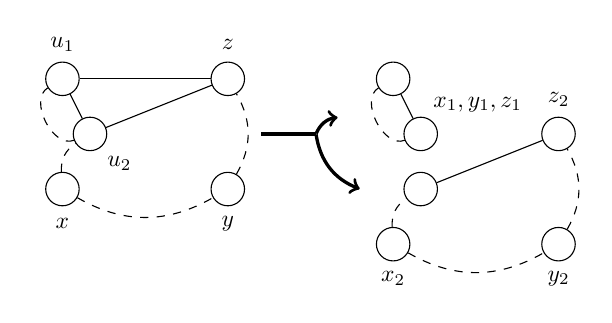
\begin{tikzpicture}[scale=1.4]
    \node (u1) at (0.0cm, 1.0cm) [label=above:${u_1}$] {};
    \node (v) at (0.25cm, 0.5cm) [label=below right:${u_2}$] {};
    \node (z) at (1.5cm, 1.0cm) [label=above:${z}$] {};
    \node (x) at (0.0cm, 0.0cm) [label=below:${x}$] {};
    \node (y) at (1.5cm, 0.0cm) [label=below:${y}$] {};

    \begin{pgfonlayer}{bg}
        \draw (z) edge (u1);
        \draw (z) edge (v);
        \draw (u1) edge (v);
        \draw (v) edge [dashed, bend left=85] (u1);
        \draw (y) edge [dashed, bend right] (z);
        \draw (x) edge [dashed, bend left] (v);
        \draw (x) edge [dashed, bend right] (y);
    \end{pgfonlayer}

    \node (bs) at (1.8cm, 0.5cm) [draw=none, fill=none, minimum size=0mm] {};
    \node (bm) at (2.3cm, 0.5cm) [draw=none, fill=none, minimum size=0mm] {};
    \node (be1) at (2.5cm, 0.65cm) [draw=none, fill=none, minimum size=0mm] {};
    \node (be2) at (2.7cm, 0.0cm) [draw=none, fill=none, minimum size=0mm] {};

    \draw (bs) edge [very thick] (bm);
    \draw (bm) edge[very thick, ->, bend left] (be1);
    \draw (bm) edge[very thick, ->, bend right] (be2);

    \node (u1b) at (3.0cm, 1.0cm) {};
    \node (vb) at (3.25cm, 0.5cm) [label=above right:${x_1,y_1,z_1}$] {};

    \node (vbp) at (3.25cm, 0.0cm) {};
    \node (zbp) at (4.5cm, 0.5cm) [label=above:${z_2}$] {};
    \node (xbp) at (3.0cm, -0.5cm) [label=below:${x_2}$] {};
    \node (ybp) at (4.5cm, -0.5cm) [label=below:${y_2}$] {};

    \begin{pgfonlayer}{bg}
        \draw (u1b) edge (vb);
        \draw (vb) edge [dashed, bend left=85] (u1b);

        \draw (zbp) edge (vbp);
        \draw (ybp) edge [dashed, bend right] (zbp);
        \draw (xbp) edge [dashed, bend left] (vbp);
        \draw (xbp) edge [dashed, bend right] (ybp);
    \end{pgfonlayer}
\end{tikzpicture}
$\quad$
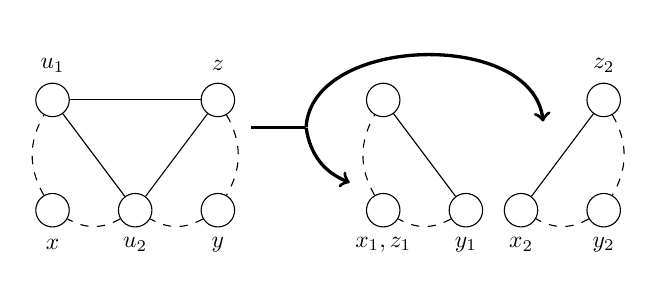
\begin{tikzpicture}[scale=1.4]
    \node (u1) at (0.0cm, 1.0cm) [label=above:${u_1}$] {};
    \node (y) at (1.5cm, 0.0cm) [label=below:${y}$] {};
    \node (z) at (1.5cm, 1.0cm) [label=above:${z}$] {};
    \node (x) at (0.0cm, 0.0cm) [label=below:${x}$] {};
    \node (v) at (0.75cm, 0.0cm) [label=below:${u_2}$] {};

    \begin{pgfonlayer}{bg}
        \draw (z) edge (u1);
        \draw (z) edge (v);
        \draw (u1) edge (v);
        \draw (z) edge [dashed, bend left] (y);
        \draw (y) edge [dashed, bend left] (v);
        \draw (v) edge [dashed, bend left] (x);
        \draw (x) edge [dashed, bend left] (u1);
    \end{pgfonlayer}

    \node (bs) at (1.8cm, 0.75cm) [draw=none, fill=none, minimum size=0mm] {};
    \node (bm) at (2.3cm, 0.75cm) [draw=none, fill=none, minimum size=0mm] {};
    \node (be1) at (4.45cm, 0.8cm) [draw=none, fill=none, minimum size=0mm] {};
    \node (be2) at (2.7cm, 0.25cm) [draw=none, fill=none, minimum size=0mm] {};

    \draw (bs) edge [very thick] (bm);
    \draw (bm) edge[very thick, ->, bend left=85] (be1);
    \draw (bm) edge[very thick, ->, bend right] (be2);

    \node (u1b) at (3.0cm, 1.0cm) {};
    \node (xb) at (3.0cm, 0.0cm) [label=below:${x_1,z_1}$] {};
    \node (vb) at (3.75cm, 0.0cm) [label=below:${y_1}$] {};

    \node (zbp) at (5.0cm, 1.0cm) [label=above:${z_2}$] {};
    \node (vbp) at (4.25cm, 0.0cm) [label=below:${x_2}$] {};
    \node (ybp) at (5.0cm, 0.0cm) [label=below:${y_2}$] {};

    \begin{pgfonlayer}{bg}
        \draw (u1b) edge (vb);
        \draw (vb) edge [dashed, bend left] (xb);
        \draw (xb) edge [dashed, bend left] (u1b);

        \draw (zbp) edge (vbp);
        \draw (zbp) edge [dashed, bend left] (ybp);
        \draw (ybp) edge [dashed, bend left] (vbp);
    \end{pgfonlayer}\end{tikzpicture}
\caption{The proof of Lemma~\ref{L:hartman3}, Case~3.2.1 (left) and
Case~3.2.2 (right).}
\end{center}
\end{figure}

\textbf{Case 3.2.1.}
Suppose that $u_2\in C(x,z)$. Observe that $x,y,z\in C_2$.
Apply the inductive hypothesis to produce a path $L$-coloring
$c_2$ of $G_2$ with designated
vertices $x_2=x$, $y_2=y$, and $z_2=z$.
Define $L'(u_2)=\{c_2(u_2)\}$ and $L'(v)=L(v)$ for each
$v\in G_1-u_2$. Apply the inductive hypothesis to produce a path $L'$-coloring
$c_1$ of $G_1$ with the single designated vertex $x_1=y_1=z_1=u_2$. Since 
$\text{deg}_{c_1}(u_2)=0$, it follows that $c$ is a path $L$-coloring of $G$
satisfying the lemma.

%\begin{figure}[ht]
%\begin{center}
%\begin{tikzpicture}[scale=1.4]
%    \node (u1) at (0.0cm, 1.0cm) [label=above:${u_1}$] {};
%    \node (y) at (1.5cm, 0.0cm) [label=below:${y}$] {};
%    \node (z) at (1.5cm, 1.0cm) [label=above:${z}$] {};
%    \node (x) at (0.0cm, 0.0cm) [label=below:${x}$] {};
%    \node (v) at (0.75cm, 0.0cm) [label=below:${u_2}$] {};
%
%    \begin{pgfonlayer}{bg}
%        \draw (z) edge (u1);
%        \draw (z) edge (v);
%        \draw (u1) edge (v);
%        \draw (z) edge [dashed, bend left] (y);
%        \draw (y) edge [dashed, bend left] (v);
%        \draw (v) edge [dashed, bend left] (x);
%        \draw (x) edge [dashed, bend left] (u1);
%    \end{pgfonlayer}
%
%    \node (bs) at (1.8cm, 0.75cm) [draw=none, fill=none, minimum size=0mm] {};
%    \node (bm) at (2.8cm, 0.75cm) [draw=none, fill=none, minimum size=0mm] {};
%    \node (be1) at (4.95cm, 0.8cm) [draw=none, fill=none, minimum size=0mm] {};
%    \node (be2) at (3.2cm, 0.25cm) [draw=none, fill=none, minimum size=0mm] {};
%
%    \draw (bs) edge (bm);
%    \draw (bm) edge[->, bend left=85] (be1);
%    \draw (bm) edge[->, bend right] (be2);
%
%    \node (u1b) at (3.5cm, 1.0cm) {};
%    \node (xb) at (3.5cm, 0.0cm) [label=below:${x_1,z_1}$] {};
%    \node (vb) at (4.25cm, 0.0cm) [label=below:${y_1}$] {};
%
%    \node (zbp) at (5.5cm, 1.0cm) [label=above:${z_2}$] {};
%    \node (vbp) at (4.75cm, 0.0cm) [label=below:${x_2}$] {};
%    \node (ybp) at (5.5cm, 0.0cm) [label=below:${y_2}$] {};
%
%    \begin{pgfonlayer}{bg}
%        \draw (u1b) edge (vb);
%        \draw (vb) edge [dashed, bend left] (xb);
%        \draw (xb) edge [dashed, bend left] (u1b);
%
%        \draw (zbp) edge (vbp);
%        \draw (zbp) edge [dashed, bend left] (ybp);
%        \draw (ybp) edge [dashed, bend left] (vbp);
%    \end{pgfonlayer}\end{tikzpicture}
%    \caption{The proof of Lemma~\ref{L:hartman3}, Case~3.2.2.}
%\end{center}
%\end{figure}

\textbf{Case 3.2.2.}
Suppose that $u_2\in C(y,x)-x-y$. Pick $c(u_2)\in L(u_2)-c(z)$. Define
$L'(u_2)=\{c(u_2)\}$ and $L'(v)=L(v)$ for each $v\in G-u_2$. 
Observe that
$x\in C_1$ and $z,y\in C_2$. Apply the inductive hypothesis to produce path
$L'$-coloring $c_1$ of
$G_1$ with designated vertices $x_1=z_1=x$ and $y_1=u_2$.
Then find a path
$L'$-coloring $c_2$ of $G_2$ with designated vertices $x_2=u_2$, $y_2=y$, and
$z_2=z$. Note that $\text{deg}_{c_1}(u_2)\le 1$ and
$\text{deg}_{c_2}(u_2)\le 1$, and thus $c$ is a path $L$-coloring of $G$
satisfying the lemma.

\begin{figure}[ht]
\begin{center}
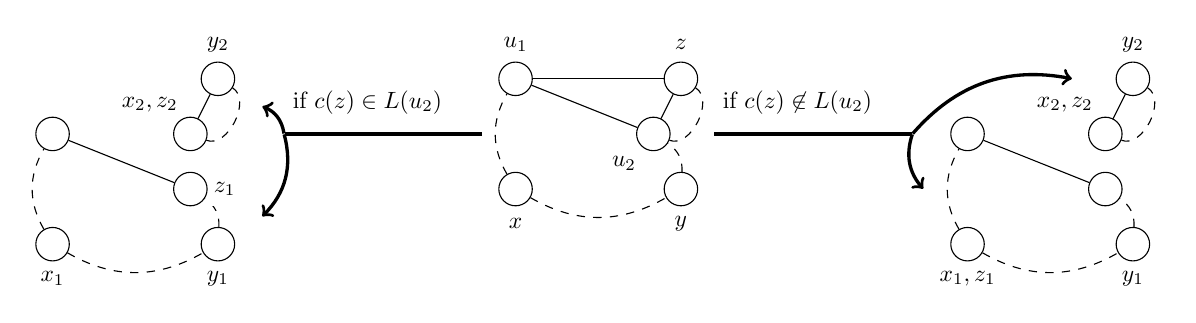
\begin{tikzpicture}[scale=1.4]
    \node (vb) at (-2.95cm, 0.5cm) [label=above left:${x_2,z_2}$] {};
    \node (zb) at (-2.7cm, 1.0cm) [label=above:${y_2}$] {};

    \node (u1bp) at (-4.2cm, 0.5cm) {};
    \node (vbp) at (-2.95cm, 0.0cm) [label=right:${z_1}$] {};
    \node (xbp) at (-4.2cm, -0.5cm) [label=below:${x_1}$] {};
    \node (ybp) at (-2.7cm, -0.5cm) [label=below:${y_1}$] {};

    \begin{pgfonlayer}{bg}
        \draw (zb) edge (vb);
        \draw (vb) edge [dashed, bend right=85] (zb);

        \draw (vbp) edge (u1bp);
        \draw (ybp) edge [dashed, bend right] (vbp);
        \draw (xbp) edge [dashed, bend left] (u1bp);
        \draw (xbp) edge [dashed, bend right] (ybp);
    \end{pgfonlayer}

    \node (cs) at (-0.3cm, 0.5cm) [draw=none, fill=none, minimum size=0mm] {};
    \node (cm) at (-2.1cm, 0.5cm) [draw=none, fill=none, minimum size=0mm] {};
    \node (ce1) at (-2.3cm, 0.75cm) [draw=none, fill=none, minimum size=0mm] {};
    \node (ce2) at (-2.3cm, -0.25cm) [draw=none, fill=none, minimum size=0mm] {};

    \draw (cs) edge [very thick]
        node[above=0.2cm, shape=rectangle, draw=none, fill=white,
                text width=2.7cm]
            {if $c(z)\in L(u_2)$}
        (cm);
    \draw (cm) edge[very thick, ->, bend right] (ce1);
    \draw (cm) edge[very thick, ->, bend left] (ce2);

    \node (u1) at (0.0cm, 1.0cm) [label=above:${u_1}$] {};
    \node (v) at (1.25cm, 0.5cm) [label=below left:${u_2}$] {};
    \node (z) at (1.5cm, 1.0cm) [label=above:${z}$] {};
    \node (x) at (0.0cm, 0.0cm) [label=below:${x}$] {};
    \node (y) at (1.5cm, 0.0cm) [label=below:${y}$] {};

    \begin{pgfonlayer}{bg}
        \draw (z) edge (u1);
        \draw (z) edge (v);
        \draw (u1) edge (v);
        \draw (v) edge [dashed, bend right=85] (z);
        \draw (y) edge [dashed, bend right] (v);
        \draw (x) edge [dashed, bend left] (u1);
        \draw (x) edge [dashed, bend right] (y);
    \end{pgfonlayer}

    \node (bs) at (1.8cm, 0.5cm) [draw=none, fill=none, minimum size=0mm] {};
    \node (bm) at (3.6cm, 0.5cm) [draw=none, fill=none, minimum size=0mm] {};
    \node (be1) at (5.05cm, 1.0cm) [draw=none, fill=none, minimum size=0mm] {};
    \node (be2) at (3.7cm, 0.0cm) [draw=none, fill=none, minimum size=0mm] {};

    \draw (bs) edge [very thick]
        node[above=0.2cm, shape=rectangle, draw=none, fill=white,
                text width=2.7cm]
            {if $c(z)\not\in L(u_2)$}
        (bm);
    \draw (bm) edge[very thick, ->, bend left] (be1);
    \draw (bm) edge[very thick, ->, bend right] (be2);

    \node (vb) at (5.35cm, 0.5cm) [label=above left:${x_2,z_2}$] {};
    \node (zb) at (5.6cm, 1.0cm) [label=above:${y_2}$] {};

    \node (u1bp) at (4.1cm, 0.5cm) {};
    \node (vbp) at (5.35cm, 0.0cm) {};
    \node (xbp) at (4.1cm, -0.5cm) [label=below:${x_1,z_1}$] {};
    \node (ybp) at (5.6cm, -0.5cm) [label=below:${y_1}$] {};

    \begin{pgfonlayer}{bg}
        \draw (zb) edge (vb);
        \draw (vb) edge [dashed, bend right=85] (zb);

        \draw (vbp) edge (u1bp);
        \draw (ybp) edge [dashed, bend right] (vbp);
        \draw (xbp) edge [dashed, bend left] (u1bp);
        \draw (xbp) edge [dashed, bend right] (ybp);
    \end{pgfonlayer}
\end{tikzpicture}
    \caption{The proof of Lemma~\ref{L:hartman3}, Case~3.2.3.}
\end{center}
\end{figure}

\textbf{Case 3.2.3.}
Suppose that $u_2\in C(z,y)$. Note that $z\ne y$. There are two distinct cases to consider.

\textbf{Case 3.2.3.1.} Suppose that $c(z)\in L(u_2)$. Then 
either $u_2=y$ and $L(z)\cap L(y)=\{c(z)\}$, or $C(z,y)\ne z,y$.
Define $L'(u_2)=\{c(z)\}$
and $L'(v)=L(v)$ for each $v\in G-u_2$. Construct a path $L'$-coloring $c_1$ of $G_1$
with designated vertices $x_1=x$,
$y_1=y$, and $z_1=u_2$. Similarly, construct a path $L'$-coloring $c_2$ of
$G_2$ with designated vertices $x_2=u_2$, $y_2=z$, and $z_2=u_2$. Since
$\text{deg}_{c_1}(u_2)\le 1$ and $\text{deg}_{c_2}(u_2)=1$, it follows
that $c$ is a path $L$-coloring of $G$.

\textbf{Case 3.2.3.2.} Suppose that $c(z)\not\in L(u_2)$. Find a path $L$-coloring
$c_1$ of $G_1$ with designated vertices
$x_1=x$, $y_1=y$, and $z_1=x$. Define $L'(u_2)=\{c_1(u_2)\}$ and $L'(v)=L(v)$
for each $v\in G_2-u_2$. Find a path $L'$-coloring $c_2$ of $G_2$
with designated vertices $x_2=u_2$, $y_2=z$, and $z_2=u_2$. Because
$C(z_2,y_2)=z_2,y_2$ and $L'(z_2)\cap L'(y_2)=\emptyset$, it is
guaranteed that $\text{deg}_{c_2}(u_2)=\text{deg}_{c_2}(z_2)=0$. Thus
$c$ is a path $L$-coloring of $G$.

Suppose that $C(z,y)=z,y$. Then it must be that $u_2=y$ and $k=2$.
Therefore $G_2=C_2=z,y$ and $\text{deg}_c(z)=0$ since $c(z)\not\in L(u_2)$.\ggcnopf
\end{proof}

%Our strategy will be to apply the inductive hypothesis
%to the blocks of $G-z$.
%Note that each cut-vertex of $G-z$
%must be a neighbor of $z$ in $C$.
%Thus each cut-vertex is contained in at most two
%two blocks, and the block-cut tree of $G-z$ is a path.
%Label the blocks $H_1,H_2,\ldots,H_{k-1}$ in counter-clockwise
%order from $z$ around $C$. Similarly label the neighbors
%of $z$ in counter-clockwise order as $u_1,\ldots,u_{k}$.
%The neighbors $u_2,\ldots,u_{k-1}$ are the cut-vertices of $G-z$, and each
%$u_\ell$ is contained in $H_{\ell-1}$ and $H_{\ell}$. See
%Figure~\ref{F:hartman3_abst} for a sketch, and Figure~\ref{F:hartman3} for a
%concrete example.
%
%Suppose that $u_1=y$. Since $z\in C(x,y)$, it must be that $x=z$.
%Define $L'(x)=\{c(x)\}$, $L'(y)=\{c(y)\}$,
%and $L'(v)=L(v)$ for all $v\in G-x-y$. 
%If $c(x)=c(y)$, then we re-label $x'=y$, $y'=x$, and $z'=x$,
%and apply the lemma with $L'$, $x'$, $y'$, and $z'$.
%Note that $x$ and $y$ will have no
%neighbors other than each other
%that share their color. If $c(y)\ne c(x)$, then instead re-label $x'=y$,
%$y'=x$, and $z'=y$. Note that since $C(z',y')=z'$, we are guaranteed that
%$\text{deg}_c(z')=0$. From now on, assume that $u_1\ne y$.
%
%If $z\ne x$ then let $H_i$ be the block 
%containing $x$; if $x=u_i$ is a cut-vertex, and is therefore
%contained two blocks $H_i$ and $H_{i+1}$, we
%single out the block $H_i$.
%If $z=x$, define $i=1$.
%
%Similarly, if $z\ne y$ define $H_j$ to be the
%block containing $y$; if $y=u_{j+1}$ is a cut-vertex, then pick
%the block $H_j$ ($j>0$ since $u_1\ne y$).
%If $z = y$ then define $j=k-1$. In all cases $1\le i\le j< k$.
%
%For any $a,b\in\{1,2,\ldots,k-1\}$
%such that $a\le b$ define
%$$ G_{a,b}=G\left[\{z\}\cup V(H_a)\cup V(H_{a+1})\cup \ldots\cup V(H_b)\right].$$ 
%In other words, $G_{a,b}$ is the induced subgraph of the set
%$\{z\}\cup \bigcup_{\ell=a}^bV(H_\ell)$ on $G$.
%
%We will path $L$-choose the blocks of $G-z$ in the order
%$$H_i\rightarrow H_{i+1}\rightarrow
%    \ldots\rightarrow H_j\rightarrow
%    H_{i-1}\rightarrow H_{i-2}\rightarrow\ldots
%    \rightarrow H_1$$
%to produce a path $L$-coloring of $G_{1,j}$. Finally,
%if $j < k-1$, we will
%path $L$-choose $G_{j+1,k-1}$ as a separate case.
%
%\begin{figure}[ht]
%\begin{center}
%\begin{tikzpicture}[scale=1.2]
%    \node (z) at (0.0cm, 1.5cm) [label=above:${z}$] {};
%    \node (u1) at (-2.0cm, 1.5cm) [label=above:${u_1}$] {};
%    \node (u2) at (-2.0cm, 0.5cm) [label=left:${u_2}$] {};
%    \node (uim1) at (-1.85cm, -0.0cm) [label=below left:${u_{i-1}}$] {};
%    \node (ui) at (-1.0cm, -0.75cm) [label=below left:${u_i}$] {};
%    \node (x) at (-0.5cm, -1.0cm) [label=below:${x}$] {};
%    \node (y) at (0.5cm, -1.0cm) [label=below:${y}$] {};
%    \node (ui1) at (1.0cm, -0.75cm) [label=below right:${u_{i+1}}$] {};
%    \node (uk) at (2.0cm, 1.5cm) [label=above:${u_k}$] {};
%
%    \node (H1) at (-1.9cm, 1.0cm) [draw=none] {$H_1$};
%    \node (Him1) at (-1.35cm, -0.32cm) [draw=none] {$H_{i-1}$};
%    \node (Hi) at (0.0cm, -0.6cm) [draw=none] {$H_i$};
%    \node (Gj1k1) at (1.25cm, 0.75cm) [draw=none] {$G_{i+1,k-1}$};
%
%    \begin{pgfonlayer}{bg} 
%        \draw (z) edge (u1);
%        \draw (z) edge (u2);
%        \draw (z) edge (uim1);
%        \draw (z) edge (ui);
%        \draw (z) edge (ui1);
%        \draw (z) edge (uk);
%
%        \draw (u2) edge [dashed] (uim1);
%
%        \draw (u1) edge [dashed, bend left=60] (u2);
%        \draw (u2) edge [dashed, bend left] (u1);
%
%        \draw (ui) edge [dashed, bend left] (uim1);
%        \draw (uim1) edge [dashed, bend left=65] (ui);
%
%        \draw (ui) edge [dashed, bend left=60] (ui1);
%        \draw (ui1) edge [dashed] (y);
%        \draw (y) edge [dashed] (x);
%        \draw (x) edge [dashed] (ui);
%
%        \draw (ui1) edge [dashed, bend right] (uk);
%    \end{pgfonlayer}
%
%    \node (zb) at (5.0cm, 1.5cm) [label=above:${z}$] {};
%    \node (u1b) at (3.0cm, 1.5cm) [label=above:${u_1}$] {};
%    \node (u2b) at (3.0cm, 0.5cm) [label=left:${u_2}$] {};
%    \node (uim1b) at (3.0cm, -0.0cm) [label=below left:${u_{i-1}}$] {};
%    \node (uib) at (3.5cm, -0.75cm) [label=below left:${u_i}$] {};
%    \node (xb) at (3.75cm, -1.25cm) [label=below left:${x}$] {};
%    \node (ui1b) at (4.3cm, -1.25cm) [label=below:${u_{i+1}}$] {};
%    \node (ui2b) at (5.25cm, -1.25cm) [label=below:${u_{i+2}}$] {};
%    \node (ujm1b) at (5.75cm, -1.1cm) [label=below right:${u_{j-1}}$] {};
%    \node (ujb) at (6.6cm, -0.6cm) [label=below right:${u_j}$] {};
%    \node (yb) at (7.0cm, -0.2cm) [label=below right:${y}$] {};
%    \node (uj1b) at (7.0cm, 0.5cm) [label=below right:${u_{j+1}}$] {};
%    \node (ukb) at (7.0cm, 1.5cm) [label=above:${u_k}$] {};
%
%    \node (H1b) at (3.1cm, 1.0cm) [draw=none] {$H_1$};
%    \node (Hi1b) at (3.35cm, -0.35cm) [draw=none] {$H_{i-1}$};
%    \node (Hib) at (3.95cm, -0.95cm) [draw=none] {$H_i$};
%    \node (Hi1b) at (4.8cm, -1.2cm) [draw=none] {$H_{i+1}$};
%    \node (Hjm1b) at (6.125cm, -0.8cm) [draw=none] {$H_{j-1}$};
%    \node (Hjb) at (6.65cm, 0.0cm) [draw=none] {$H_j$};
%    \node (Gj1k1b) at (6.35cm, 1.2cm) [draw=none] {$G_{j+1,k-1}$};
%
%    \begin{pgfonlayer}{bg} 
%        \draw (zb) edge (u1b);
%        \draw (zb) edge (u2b);
%        \draw (zb) edge (uim1b);
%        \draw (zb) edge (uib);
%        \draw (zb) edge (ui1b);
%        \draw (zb) edge (ui2b);
%        \draw (zb) edge (ujm1b);
%        \draw (zb) edge (ujb);
%        \draw (zb) edge (uj1b);
%        \draw (zb) edge (ukb);
%
%        \draw (u2b) edge [dashed] (uim1b);
%
%        \draw (u1b) edge [dashed, bend left=60] (u2b);
%        \draw (u2b) edge [dashed, bend left] (u1b);
%
%        \draw (uib) edge [dashed, bend left] (uim1b);
%        \draw (uim1b) edge [dashed, bend left=65] (uib);
%
%        \draw (uib) edge [dashed, bend left=60] (ui1b);
%        \draw (ui1b) edge [dashed] (xb);
%        \draw (xb) edge [dashed] (uib);
%
%        \draw (ui1b) edge [dashed, bend left=60] (ui2b);
%        \draw (ui2b) edge [dashed, bend left] (ui1b);
%
%        \draw (ui2b) edge [dashed] (ujm1b);
%
%        \draw (ujm1b) edge [dashed, bend left=60] (ujb);
%        \draw (ujb) edge [dashed, bend left] (ujm1b);
%
%        \draw (ujb) edge [dashed, bend left=60] (uj1b);
%        \draw (uj1b) edge [dashed] (yb);
%        \draw (yb) edge [dashed] (ujb);
%
%        \draw (uj1b) edge [dashed] (ukb);
%    \end{pgfonlayer}
%\end{tikzpicture}
%\caption{A sketch of the graph structure in the proof of Lemma~\ref{L:hartman3}
%in the case $i=j$ (left) and the case $i\ne j$ (right).}
%\label{F:hartman3_abst}
%\end{center}
%\end{figure}
%
%\textbf{Step 1.} To start we will path $L$-choose $G_{i,i}$.
%
%\textbf{Case 1.1.} Suppose that $i=j$ and therefore
%$G_{i,i}=G_{i,j}$. If $z=y$ or $c(z)\not\in L(u_{i+1})$,
%define $L_i(v)=L(v)-\{c(z)\}$
%for all $v\in N(z)\cap V(H_i)$, and $L_i(v)=L(v)$ for all
%$v\in V(H_i)-N(z)$. If $z=y$, define
%$y_i=u_{i+1}$, otherwise $y_i=y$. Similarly, if $x=z$, define $x_i=u_i$,
%otherwise $x_i=x$. Note that either $y_i=u_{i+1}$ or $|L_i(u_{i+1})|\ge 2$.
%Define $z_i=x_i$ and apply the inductive hypothesis to path
%$L_i$-choose $H_i$ with the designated vertices $x_i$, $y_i$, and $z_i$.
%The $L_i$-choosing
%extends to a path $L$-coloring of $G_{i,j}$ with
%$\text{deg}_c(x)\le 1$, $\text{deg}_c(y)\le 1$, and $\text{deg}_c(z)=0$.
%
%Otherwise $z\ne y$ and $c(z)\in L(u_{i+1})$. Define
%$L_i(u_{i+1})=\{c(z)\}$, define $L_i(v)=L(v)-\{c(z)\}$ for
%$v\in N(z)\cap V(H_i-u_{i+1})$, and define $L_i(v)=L(v)$
%for all $v\in V(H_i)-N(z)$. If $x=z$, define $x_i=u_i$, otherwise define $x_i=x$.
%Define $y_i=y$ and $z_i=u_{i+1}$.
%Path $L_i$-choose $H_i$ with
%$x_i$, $y_i$, and $z_i$. The $L_i$-choosing of $H_i$ extends to a path
%$L$-coloring of $G_{i,j}$ such that $\text{deg}_c(x)\le 1$,
%$\text{deg}_c(y)\le 1$, and $\text{deg}_c(z)=1$.
%
%\textbf{Case 1.2.} Suppose that $i\ne j$.
%Define $L_i(v)=L(v)-\{c(z)\}$ for all $v\in N(z)\cap V(H_i)$,
%and $L_i(v)=L(v)$ for all $v\in V(H_i)-N(z)$. 
%If $z=x$ or if $x=u_i$ is a cut-vertex, then we
%define $x_i=u_i$, $z_i=u_i$, and $y_i=u_{i+1}$ and path $L_i$-choose $H_i$.
%Note that if $z=x$ then $i=1$ and $x_1=u_1$
%is the vertex immediately counter-clockwise to $z$ around $C$.
%
%Otherwise $x$ is not a cut-vertex. Note that $u_i\in C(x,z) - z$ and
%therefore $|L'(u_i)|\ge 2$. Thus we may define $x_i=x$, $z_i=x$,
%$y_i=u_{i+1}$ and path $L_i$-choose $H_i$.
%
%In both cases the path $L_i$-choosing of $H_i$ extends to a path
%$L$-coloring of $G_{i,i}$ such that $\text{deg}_c(u_{i+1})\le 1$,
%$\text{deg}_c(x)\le 1$, and $\text{deg}_c(z)=0$.
%
%\textbf{Step 2.} Suppose that $\ell\in\{i+1, i+2,\ldots,j-1\}$
%and we have computed a path $L$-coloring of $G_{i,\ell-1}$ such that
%$\text{deg}_c(u_\ell)\le1$, $\text{deg}_c(x)\le 1$,
%and $\text{deg}_c(z)=0$.
%
%Define $L_\ell(u_\ell)=\{c(u_\ell)\}$,
%$L_\ell(v)=L(v)-\{c(z)\}$ for
%all $v\in N(z)\cap V(H_\ell-u_\ell)$, and
%$L_\ell(v)=L(v)$ for all $v\in V(H_\ell)-N(z)$.
%Path $L_\ell$-choose $H_\ell$ with
%$x_\ell=u_\ell$, $z_\ell=u_\ell$, and
%$y_\ell=u_{\ell+1}$. We are guaranteed that the path $L$-coloring
%of $G_{i,\ell-1}$ and the path $L_\ell$-choosing of $H_\ell$ agree
%at the shared vertex $u_\ell$, and that
%$\text{deg}_c(u_\ell)\le 1$ and $\text{deg}_c(u_{\ell+1})\le 1$
%in $H_\ell$. Taken together they form a
%path $L$-list coloring of $G_{i,\ell}$ with $\text{deg}_c(u_{\ell+1})\le 1$,
%$\text{deg}_c(x)\le 1$, and $\text{deg}_c(z)=0$.
%
%\textbf{Step 3.} Suppose that $i\ne j$ and we
%have computed a path $L$-coloring of $G_{i,j-1}$ such that
%$\text{deg}_c(u_j)\le1$, $\text{deg}_c(x)\le 1$, and $\text{deg}_c(z)=0$. 
%
%If $z=y$, then
%define $x_j=u_j$, $z_j=u_j$, $y_j=u_{j+1}$,
%$L_j(v)=L(v)-\{c(z)\}$ for all $v\in N(z)\cap V(H_j)$,
%and $L_j(v)=L(v)$ for all $v\in V(H_j)-N(z)$. Path 
%$L_j$-choose
%$H_j$ and note that it extends to form a path
%$L$-coloring of $G_{i,j}$ with
%$\text{deg}_c(z)=0$ via the same argument from Step 2.
%
%Otherwise $z\ne y$ and $u_{j+1}$ is the furthest clockwise neighbor of $z$
%around $C$ in $C(z,y)$. If $c(z)\in L(u_{j+1})$, then define
%$L_j(u_{j+1})=\{c(z)\}$, $L_j(v)=L(v)-\{c(z)\}$ for all $v\in
%N(z)\cap(H_j-u_{j+1})$, and $L_j(v)=L(v)$ for all
%$v\in V(H_j)-N(z)$. Path $L_j$-choose $H_j$ with $x_j=u_j$,
%$z_j=u_{j+1}$, and $y_j=y$. The path $L_j$-choosing of $H_j$
%agrees with the path $L$-coloring
%of $G_{i,j-1}$, and both combine to form a path $L$-coloring
%of $G_{i,j}$ such that $\text{deg}_c(x)\le 1$, $\text{deg}_c(y)\le 1$,
%and $\text{deg}_c(z)=1$.
%
%If $c(z)\not\in L(u_{j+1})$,
%then define $L_j(v)=L(v)-\{c(z\}$ for all $v\in N(z)\cap V(H_j)$,
%and $L_j(v)=L(v)$ for all $v\in V(H_j)-N(z)$. Note that
%$|L_j(u_{j+1})|\ge 2$, thus we may path $L_j$-choose $H_j$ with
%$x_j=u_j$, $z_j=u_j$, and $y_j=y$. The $L_j$-choosing extends to path
%$L$-coloring of $G_{i,j}$ with $\text{deg}_c(x)\le 1$, $\text{deg}_c(y)\le 1$,
%and $\text{deg}_c(z)=0$.
%
%\textbf{Step 4.} We will
%now color any remaining blocks $H_\ell$ with
%$\ell<i$. Suppose that $\ell\in \{1,2,..,i-1\}$ and that we have
%computed a path
%$L$-coloring of $G_{\ell+1,j}$ such that $\text{deg}_c(z)\le 1$. Define
%$L_\ell(u_{\ell+1})=\{c(u_{\ell+1})\}$,
%$L_\ell(v)=L(v)-\{c(z)\}$
%for all $v\in N(z)\cap V(H_\ell-u_{\ell+1})$,
%and $L_\ell(v)=L(v)$ for $v\in V(H_\ell)-N(z)$. Path $L_\ell$-choose $H_\ell$ with
%$x_\ell=u_{\ell+1}$, $y_\ell=u_{\ell+1}$, and $z_\ell=u_{\ell+1}$.
%Note that $\text{deg}_c(u_{\ell+1})=0$ in $H_\ell$. Therefore the
%$L_\ell$-choosing
%extends to a path $L$-coloring of $G_{\ell,j}$ such that no vertex
%in $G_{\ell+1,j}$ shares a color with a neighbor in $H_\ell-u_{\ell+1}$.
%
%\textbf{Step 5.} If $j=k-1$, then the above steps have produced a path
%$L$-coloring of $G$. Otherwise it remains to extend the $L$-coloring of
%$G_{1,j}$ to $G_{j+1,k-1}$.
%
%Define $L'(u_{j+1})=\{c(u_{j+1})\}$, $L'(z)=\{c(z)\}$, and $L'(v)=L(v)$ for
%$v\in G_{j+1,k-1}-u_{j+1} -z$. 
%Path $L'$-choose $G'=G_{j+1,k-1}$ with $x'=u_{j+1}$,
%$z'=u_{j+1}$, and $y'=z$. Let $C'$ be the outer face of $G'$.
%
%By Step 4 either $\text{deg}_c(z)=0$ in $G_{1,j}$ or
%$c(u_{j+1})=c(z)$ and $\text{deg}_c(z)=1$ in $G_{1,j}$.
%Moreover, since $z'=u_{j+1}$,
%we are guaranteed that the only neighbors of
%$u_{j+1}$ in $G'$ that share a color with $u_{j+1}$ are in
%$C'(z',y')=C'(u_{j+1},z)$.
%But $C'(u_{j+1},z)=u_{j+1},z$, so either $c(z)=c(u_{j+1})$
%and $\text{deg}_c(u_{j+1})=1$ in $G'$, or $c(z)\ne c(u_{j+1})$ and
%$\text{deg}_c(u_{j+1})=0$ in $G'$.
%Because
%$$V(G_{1,j})\cap V(G_{j+1,k-1})=\{z,u_{j+1}\}=\{x',y'\},$$
%it follows that the path
%$L$-coloring of $G_{1,j}$ and the path $L'$-choosing of $G_{j+1,k-1}$
%agree and extend to a path $L$-coloring of $G$ such that
%$\text{deg}_c(x)\le1$,
%$\text{deg}_c(y)\le 1$, and $\text{deg}_c(z)\le 1$.\ggcnopf
%\end{proof}
%
%\begin{figure}[ht]
%\begin{center}
%\begin{tikzpicture}[scale=1.2]
%    \node (z) [label=above:$1$] at (0.0cm, 1.5cm) {$z$};
%    \node (u0) [label=above:${2,3}$] at (-2.0cm, 1.5cm) {$u_1$};
%    \node (v0) [label=above:${2,4,5}$] at (-1.5cm, 1.0cm) {};
%    \node (u1) [label=left:${4,5}$] at (-2.0cm, 0.5cm) {$u_2$};
%    \node (v1) [label=above:${1,5,7}$] at (-0.5cm, 0.5cm) {};
%    \node (v2) [label=left:$3$] at (-2.0cm, -0.5cm) {$x$};
%    \node (v3) [label=above:${2,4,6}$] at (-1.5cm, -0.5cm) {};
%    \node (v4) [label=below:${3,4,5}$] at (-1.0cm, -0.5cm) {};
%    \node (u2) [label=below:${1,2}$] at (-0.5cm, -1.5cm) {$u_3$};
%    \node (v5) [label=above:${1,2,3}$] at (0.0cm, -0.5cm) {};
%    \node (u3) [label=below:${1,2}$] at (0.5cm, -1.5cm) {$u_4$};
%    \node (v6) [label=right:$1$] at (1.0cm, -0.5cm) {$y$};
%    \node (v7) [label=above:${2,6,7}$] at (0.75cm, 0.0cm) {};
%    \node (u4) [label=right:${1,6}$] at (1.5cm, 0.5cm) {$u_5$};
%    \node (u5) [label=above:${1,7}$] at (1.5cm, 1.5cm) {$u_6$};
%
%    \begin{pgfonlayer}{bg} 
%        \draw (z) edge (u0);
%        \draw (z) edge (u1);
%        \draw (z) edge (u2);
%        \draw (z) edge (u3);
%        \draw (z) edge (u4);
%        \draw (z) edge (u5);
%
%        \draw (z) edge (v0);
%        \draw (z) edge (v1);
%        \draw (z) edge (v5);
%        \draw (z) edge (v7);
%
%        \draw (u0) edge (u1);
%        \draw (u1) edge (v2);
%        \draw (v2) edge (u2);
%        \draw (u2) edge (u3);
%        \draw (u3) edge (v6);
%        \draw (v6) edge (u4);
%        \draw (u4) edge (u5);
%
%        \draw (u0) edge (v0);
%        \draw (u1) edge (v0);
%        \draw (u1) edge (v1);
%        \draw (u1) edge (v3);
%        \draw (u2) edge (v3);
%        \draw (u2) edge (v4);
%        \draw (u2) edge (v1);
%        \draw (u2) edge (v5);
%        \draw (u3) edge (v5);
%        \draw (u3) edge (v7);
%        \draw (u4) edge (v7);
%
%        \draw (v1) edge (v3);
%        \draw (v1) edge (v4);
%        \draw (v2) edge (v3);
%        \draw (v3) edge (v4);
%        \draw (v6) edge (v7);
%    \end{pgfonlayer}
%
%    \node (H0) [draw=none, scale=1.5] at (3.7cm, 1.5cm) {$H_1$};
%    \node (u0a) [label=above:${2,3}$] at (4.0cm, 2.0cm) {};
%    \node (v0a) [label=above:${2,4,5}$] at (4.5cm, 1.5cm) {};
%    \node (u1a) [label=left:${4,5}$] at (4.0cm, 1.0cm) {$z_1$};
%
%    \node (H1) [draw=none, scale=1.5] at (4.5cm, -1.25cm) {$H_2$};
%    \node (u1b) [label=left:${4,5}$] at (4.0cm, 0.5cm) {};
%    \node (v1b) [label=above right:${5,7}$] at (5.5cm, 0.5cm) {};
%    \node (v2b) [label=left:$3$] at (4.0cm, -0.5cm) {$z_2$};
%    \node (v3b) [label=above:${2,4,6}$] at (4.5cm, -0.5cm) {};
%    \node (v4b) [label=below:${3,4,5}$] at (5.0cm, -0.5cm) {};
%    \node (u2b) [label=below:$2$] at (5.5cm, -1.5cm) {$y_2$};
%
%    \node (H2) [draw=none, scale=1.5] at (6.5cm, -1.8cm) {$H_3$};
%    \node (u2c) [label=below:$2$] at (6.0cm, -1.5cm) {$z_3$}; 
%    \node (v5c) [label=above:${2,3}$] at (6.5cm, -0.5cm) {};
%    \node (u3c) [label=below:$2$] at (7.0cm, -1.5cm) {$y_3$};
%
%    \node (H3) [draw=none, scale=1.5] at (8.25cm, -1.0cm) {$H_4$};
%    \node (u3d) [label=below:$2$] at (7.5cm, -1.5cm) {$x_4$};
%    \node (v6d) [label=right:$1$] at (8.0cm, -0.5cm) {$y_4$};
%    \node (v7d) [label=above left:${2,6,7}$] at (7.75cm, 0.0cm) {};
%    \node (u4d) [label=right:$1$] at (8.5cm, 0.5cm) {$z_4$};
%
%    \node (H4) [draw=none, scale=1.5] at (9.0cm, 1.5cm) {$G_{5,5}$};
%    \node (u4e) [label=right:$1$] at (8.5cm, 1.0cm) {$z'$};
%    \node (u5e) [label=above:${1,7}$] at (8.5cm, 2.0cm) {};
%    \node (ze) [label=above:$1$] at (7.0cm, 2.0cm) {$y'$};
%
%    \begin{pgfonlayer}{bg}
%        \draw (u0a) edge (u1a);
%        \draw (u0a) edge (v0a);
%        \draw (u1a) edge (v0a);
%
%        \draw (u1a) edge [dashed] (u1b);
%
%        \draw (u1b) edge (v2b);
%        \draw (v2b) edge (u2b);
%        \draw (u1b) edge (v1b);
%        \draw (u1b) edge (v3b);
%        \draw (u2b) edge (v3b);
%        \draw (u2b) edge (v4b);
%        \draw (u2b) edge (v1b);
%        \draw (v1b) edge (v3b);
%        \draw (v1b) edge (v4b);
%        \draw (v2b) edge (v3b);
%        \draw (v3b) edge (v4b);
%
%        \draw (u2b) edge [dashed] (u2c);
%
%        \draw (u2c) edge (u3c);
%        \draw (u2c) edge (v5c);
%        \draw (u3c) edge (v5c);
%
%        \draw (u3c) edge [dashed] (u3d);
%
%        \draw (u3d) edge (v6d);
%        \draw (v6d) edge (u4d);
%        \draw (v6d) edge (v7d);
%        \draw (u3d) edge (v7d);
%        \draw (u4d) edge (v7d);
%
%        \draw (u4d) edge [dashed] (u4e);
%
%        \draw (ze) edge (u4e);
%        \draw (ze) edge (u5e);
%        \draw (u4e) edge (u5e);
%    \end{pgfonlayer}
%\end{tikzpicture}
%\caption{A concrete example step of the path $L$-coloring procedure in
%the proof of
%Lemma~\ref{L:hartman3}. Each vertex $v\in G$ is labelled with $L(v)$.
%If $z_\ell=x_\ell$
%and/or $z_\ell=y_\ell$, then only $z_\ell$ is labelled.}
%\label{F:hartman3}
%\end{center}
%\end{figure}

Let $G$ be a planar graph and $L$ a list assignment such
that $|L(v)|\ge 3$ for each $v\in G$. Compute a planar embedding and add edges
to produce a triangulated plane graph $G'$. Pick $u\in G'$ to be a vertex
on the outer face and $c(u)\in L(u)$. Define $L'$ to be the list
assignment such that $L'(u)=\{c(u)\}$ and $L'(v)=L(v)$ for $v\in G'-u$.
By Lemma~\ref{L:hartman3} there exists a path $L'$-coloring $c$ of $G'$.
Clearly $c$ is also a path $L$-coloring of $G$.
Therefore Theorem~\ref{T:planar3} follows immediately from 
Lemma~\ref{L:hartman3}.

The proof of Lemma~\ref{L:hartman3} is a constructive algorithm that may be
implemented for plane graphs represented by
rotation scheme ordered augmented adjacency lists.
We will assume that both forward and backward iteration in augmented adjacency
lists
is a constant time operation.
The
available C implementation represents each augmented adjacency list as an array
of entries~\cite{Bro2017}.

%In terms of plane graphs, given the entry for an edge $vu$
%in the rotation scheme ordered adjacency list for a vertex $v$, we assume that
%it is a
%constant time operation to retrieve the entry corresponding to the
%edge immediately clockwise or counter-clockwise from $uv$ around $v$.

%For each vertex $v\in G$ the implementation will track a list $L[v]$ of up to
%three colors,
%an integer location mark $S[v]$, and a pair $N[v]=(r_1,r_2)$ of references to
%neighbor entries in $v$'s augmented adjacency list.
%
%For each $v\in C$, $N[v]$ will contain references to the adjacency list
%entries for the vertices immediately counter-clockwise and immediately clockwise
%from $v$ around $C$. All together, the array of pairs $N$ will provide a
%representation of $C$ and $\text{Int}(C)$.
% 
%We will track the locations of vertices on the outer face by marking each vertex
%$v\in C(x,z)-z$ such that $S[v]=S[x]$, and marking each vertex $v\in C(z,y)-z$
%such that $S[v]=S[y]$. The only situation where an interior vertex becomes
%a vertex on the outer face of a subgraph $G_i$ is
%in Case~3.1. To implement Case~3.1, initialize $S[u_2]\leftarrow S[x]$
%to indicate that $u_2\in C'(x,y)$ in $G-zu_1$, and
%initialize $N[u_2]=(r_1,r_2)$ with $r_1$ a reference to the entry for $u_1$
%and $r_2$ a reference to the entry for $z$.
%
%In Case~3.2.3.2
%the segment $C_1(z_1,y_1)=C_1(x_1,y_1)$ will consist of vertices
%$v\in C(x,u_1)$ with $S[v]=S[u_x]$, and vertices $v\in C(u_2,y)$
%with $S[v]=S[y]$.
%To avoid having to iterate through and re-mark each vertex in the segment,
%we will keep track of a separate array of integers $M$
%initialized such that
%$M[i]=i$ for each mark $i$.
%Whenever a mark $S[v]$ is compared with the mark $S[y]$,
%instead compare
%$M[S[v]]$ with $S[y]$. To join the segment $C(x,u_1)$ marked with
%$S[x]$ and the segment $C(u_2,y)$ marked with $S[y]$, simply
%assign $M[S[x]]\leftarrow S[y]$.

\begin{algorithm}\label{A:hartman_impl}
\textbf{Input.} Let $C$ be a cycle or length $2$ path in a
$2$-connected, weakly triangulated plane graph $G$
represented by augmented adjacency lists. Let $x,y,z\in C$ be
vertices such that $z\in C(x,y)$.

Let $L$ be an array of lists of colors
such that for $v\in\{x,y,z\}$ the list $L[v]$ has length one,
for $v\in C-\{x,y,z\}$ the list $L[v]$ has length two
or three, and for $v\in \text{Int}(C)-C$ the list
$L[v]$ has length three. Furthermore, for each $v\in C(x,z) - z$ assume
that $L[v]$ does not contain the color in $L[z]$.

Let $N$ be an array of pairs of
references such that for each $v\in C$ the pair $N[v]=(r_1,r_2)$ contains
a reference $r_1$ to the neighbor the immediately counter-clockwise
from $v$
around $C$, and a reference $r_2$
to the neighbor immediately clockwise from $v$ around $C$.

Let $S$ be an array of
integers such that for each $v\in C(x,z)-z$ we have $S[v]=S[x]$ and for
all vertices $v\in C-C(x,z)$ we have $S[v]\ne S[x]$. Furthermore, for each
vertices $v\in C$ assume that $S[v]\ne 0$, and for each $v\in \text{Int}(C)-C$
assume that $S[v]=0$.

Finally, let $M$
be an array of integers such that for all vertices $v\in C(z,y)$ we have
$M[S[v]]=S[y]$, and for all vertices $v\in C-C(z,y)$ we have $M[S[v]]\ne
S[y]$.

\textbf{Output.} Elements will be removed from the lists in $L$ such that
for each $v\in\text{Int}(C)$ the list $L[v]$ will contain a single color. The
coloring of $\text{Int}(C)$ corresponding to the remaining
colors will be a path
coloring $c$ such that $\text{deg}_c(x)\le1$, $\text{deg}_c(y)\le1$, and
$\text{deg}_c(z)\le1$. If $z=y$, or if $C(z,y)=z,y$ and $L[z]$ doesn't contain
the color in $L[y]$, then $\text{deg}_c(z)=0$.

\textbf{Procedure.} Let $N[z]=(r_1,r_2)$. Define the vertex $u_1$ to be
the neighbor of $z$ corresponding to $r_1$.

\textbf{Base Case.} If $r_1=r_2$, then $C=z,u_1$
is a length $2$ path. If $u_1\ne x$ and $u_1\ne y$, remove the
color in $L[z]$ from $L[u_1]$. If more than one color still remains in
$L[u_1]$, remove arbitrary colors until a single color remains.

\textbf{Recursive Step.} Suppose that $r_1\ne r_2$. Note that
$n(C)>2$ and therefore $C$ is a cycle. Define $u_2$ to be the
neighbor of $z$ immediately counter-clockwise from $u_1$.

\textbf{Case 1.} Suppose that $u_1=y$. In this case it must be that
$z=x$. Assign
$S[x]$ and $S[y]$ new unique marks. Assign $M[S[x]]\leftarrow S[x]$
and $M[S[y]]\leftarrow S[y]$. Make a recursive call re-assigning
$x'\leftarrow y$, $y'\leftarrow x$, and $z'\leftarrow y$.

\textbf{Case 2.} Suppose that $z=x$ and $u_1\ne y$. 
Remove the color in $L[z]$ from $L[u_1]$, and then remove arbitrary
colors from $L[u_1]$ until a single color remains.
Assign $x\leftarrow u_1$,
set $S[u_1]$ to be a new unique mark, assign $M[S[u_1]]\leftarrow S[u_1]$,
and make a recursive call.

\textbf{Case 3.} Suppose that $z\ne x$ and $u_1\ne y$. It is this case that
makes use of the back references in the augmented adjacency list representation.

\textbf{Case 3.1.} Suppose that $S[u_2]=0$, that is, $u_2\in
\text{Int}(C)-C$. Assign $S[u_2]\leftarrow S[x]$ and initialize
$N[u_2]\leftarrow(s_1,s_2)$ where $s_1$ is a reference to the entry
for $u_1$ in $\text{Adj}[u_2]$, and $s_2$ is a reference to the entry
for $z$. Remove the color in $L[z]$ from
$L[u_2]$ and remove the edge $zu_1$ by adjusting
$N[u_1]$ and $N[z]$. Make a recursive call with $x$, $y$, and $z$ the
same as before.

\textbf{Case 3.2.} Suppose that $S[u_2]\ne 0$, that is, $u_2\in C$. Just as in
Case~3.2 of the proof of Lemma~\ref{L:hartman3}, we will separately consider
the two blocks $G_1$ and $G_2$ of $\text{Int}(C)-zu_1$.

It is simple to remove the edge $zu_1$ by adjusting $N[z]$ and $N[u_1]$ to
exclude
the corresponding entries. It remains
to ``split'' the
neighborhood of $u_2$ at the edge $u_2z$ such that the recursive call on $G_1$
considers only the neighbors of $u_2$ counter-clockwise from $z$, and the call
on $G_2$ considers $z$ and all neighbors clockwise from $z$.

Let $N[u_2]=(s_1,s_2)$. Let $s_3$ be a reference to $z$'s entry in
$\text{Adj}[u_2]$ and
$s_3+1$ a reference to the next entry counter-clockwise from $z$ in
$\text{Adj}[u_2]$.
To represent
the subgraph $G_1$ from the proof's Case~3.2, we assign
$N[u_2]\leftarrow (s_3+1,s_2)$. To represent the graph $G_2$,
we assign $N[u_2]\leftarrow (s_1,s_3)$.

\textbf{Case 3.2.1.} Suppose that $S[u_2]=S[x]$, i.e. $u_2\in C(x,z)$. Make a
recursive call on $G_2$ with $x_2\leftarrow x$,
$y_2\leftarrow y$, $z_2\leftarrow z$. Assign
$S[u_2]$ a new
unique mark, set $M[S[u_2]]\leftarrow S[u_2]$, and make a recursive call
on $G_1$ with $x_1,y_1,z_1$ all equal to $u_2$.

\textbf{Case 3.2.2.} Suppose that $z\ne x$ and $S[u_2]\ne 0$, but
$S[u_2]\ne S[x]$ and $M[S[u_2]]\ne S[y]$. In other words, suppose that $u_2\in C(y,x)-x-y$.
First remove the color in $L[z]$ from $L[u_2]$, if it exists, and then remove
arbitrary colors until $L[u_2]$ is of length one. Assign $S[u_2]=S[x]$.
Make a recursive call on $G_1$ with $x_1\leftarrow x$,
$y_1\leftarrow u_2$, and $z_1\leftarrow x$.
Assign $S[u_2]$ a new unique mark and $M[S[u_2]]\leftarrow S[u_2]$.
Make a recursive call on $G_2$
with $x_2\leftarrow u_2$, $y_2\leftarrow y$, and $z_2\leftarrow z$,
splitting $N[u_2]$ at the edge $u_2z$ to contain $z$ and all neighbors clockwise
from $z$.

\textbf{Case 3.2.3.} Suppose that $z\ne x$ and $M[S[u_2]]=S[y]$, i.e.
$u_2\in C(z,y)$. There are
two cases to consider.

\textbf{Case 3.2.3.1.} Suppose that the color in $L[z]$ is in $L[u_2]$. Remove
all colors other than the one in $L[z]$ from $L[u_2]$.
Make a recursive call on $G_1$ with $x_1\leftarrow x$,
$y_1\leftarrow y$, and $z_1\leftarrow u_2$.
Then assign $S[z]$ and $S[u_2]$ the same new unique mark, and assign
$M[S[z]]\leftarrow S[z]$. Make a
recursive call on $G_2$ with $x_2\leftarrow u_2$, $y_2\leftarrow z$,
and $z_2\leftarrow u_2$.

\textbf{Case 3.2.3.2.} Suppose that the color in $L[z]$ is not in $L[u_2]$.
Assign $M[S[x]]\leftarrow S[y]$. Make a recursive call on $G_1$
with $x_1\leftarrow x$,
$y_1\leftarrow y$, and $z_1\leftarrow x$.
Assign $S[z]$ and $S[u_2]$ the same new unique mark, and
set $M[S[z]]\leftarrow S[z]$. Make a
recursive call on $G_2$ with $x_2\leftarrow u_2$, $y_2\leftarrow z$,
and $z_2\leftarrow u_2$.
\end{algorithm}

%\begin{figure}
%\begin{center}
%\begin{tikzpicture}[scale=1.2]
%    \node (z) [label=above:${2, \{1\}}$] at (0.0cm, 1.5cm) {$z$};
%    \node (u0) [label=above:${4,\{2,3\}}$] at (-2.0cm, 1.5cm) {$u_1$};
%    \node (v0) [label=above right:${0,\{2,4,5\}}$] at (-1.5cm, 1.0cm) {$u_2$};
%    \node (u1) [label=left:${4,\{4,5\}}$] at (-2.0cm, 0.5cm) {};
%    \node (v1) [label=above:${0,\{1,5,7\}}$] at (-0.5cm, 0.5cm) {};
%    \node (v2) [label=below left:${4,\{3\}}$] at (-2.0cm, -0.5cm) {$x$};
%    \node (v3) [label=above:${0,\{2,4,6\}}$] at (-1.5cm, -0.5cm) {};
%    \node (v4) [label=below:${0,\{3,4,5\}}$] at (-1.0cm, -0.5cm) {};
%    \node (u2) [label=below:${1,\{1,2\}}$] at (-0.5cm, -1.5cm) {};
%    \node (v5) [label=above:${0,\{1,2,3\}}$] at (0.0cm, -0.5cm) {};
%    \node (u3) [label=below:${1,\{1,2\}}$] at (0.5cm, -1.5cm) {};
%    \node (v6) [label=below right:${2,\{1\}}$] at (1.0cm, -0.5cm) {$y$};
%    \node (v7) [label=above:${0,\{2,6,7\}}$] at (0.75cm, 0.0cm) {};
%    \node (u4) [label=below right:${2,\{1,6\}}$] at (1.5cm, 0.5cm) {};
%    \node (u5) [label=above:${2,\{1,7\}}$] at (1.5cm, 1.5cm) {};
%
%    \begin{pgfonlayer}{bg} 
%        \draw (z) edge (u0);
%        \draw (z) edge (u1);
%        \draw (z) edge (u2);
%        \draw (z) edge (u3);
%        \draw (z) edge (u4);
%        \draw (z) edge (u5);
%
%        \draw (z) edge (v0);
%        \draw (z) edge (v1);
%        \draw (z) edge (v5);
%        \draw (z) edge (v7);
%
%        \draw (u0) edge (u1);
%        \draw (u1) edge (v2);
%        \draw (v2) edge (u2);
%        \draw (u2) edge (u3);
%        \draw (u3) edge (v6);
%        \draw (v6) edge (u4);
%        \draw (u4) edge (u5);
%
%        \draw (u0) edge (v0);
%        \draw (u1) edge (v0);
%        \draw (u1) edge (v1);
%        \draw (u1) edge (v3);
%        \draw (u2) edge (v3);
%        \draw (u2) edge (v4);
%        \draw (u2) edge (v1);
%        \draw (u2) edge (v5);
%        \draw (u3) edge (v5);
%        \draw (u3) edge (v7);
%        \draw (u4) edge (v7);
%
%        \draw (v1) edge (v3);
%        \draw (v1) edge (v4);
%        \draw (v2) edge (v3);
%        \draw (v3) edge (v4);
%        \draw (v6) edge (v7);
%    \end{pgfonlayer}
%
%    \node (zb) [label=above:${2, \{1\}}$] at (6.0cm, 1.5cm) {$z$};
%    \node (u0b) [label=above:${4,\{2,3\}}$] at (4.0cm, 1.5cm) {};
%    \node (v0b) [label=above right:${4,\{2,4,5\}}$] at (4.5cm, 1.0cm) {$u_1$};
%    \node (u1b) [label=left:${4,\{4,5\}}$] at (4.0cm, 0.5cm) {$u_2$};
%    \node (v1b) [label=above:${0,\{1,5,7\}}$] at (5.5cm, 0.5cm) {};
%    \node (v2b) [label=below left:${4,\{3\}}$] at (4.0cm, -0.5cm) {$x$};
%    \node (v3b) [label=above:${0,\{2,4,6\}}$] at (4.5cm, -0.5cm) {};
%    \node (v4b) [label=below:${0,\{3,4,5\}}$] at (5.0cm, -0.5cm) {};
%    \node (u2b) [label=below:${1,\{1,2\}}$] at (5.5cm, -1.5cm) {};
%    \node (v5b) [label=above:${0,\{1,2,3\}}$] at (6.0cm, -0.5cm) {};
%    \node (u3b) [label=below:${1,\{1,2\}}$] at (6.5cm, -1.5cm) {};
%    \node (v6b) [label=below right:${2,\{1\}}$] at (7.0cm, -0.5cm) {$y$};
%    \node (v7b) [label=above:${0,\{2,6,7\}}$] at (6.75cm, 0.0cm) {};
%    \node (u4b) [label=below right:${2,\{1,6\}}$] at (7.5cm, 0.5cm) {};
%    \node (u5b) [label=above:${2,\{1,7\}}$] at (7.5cm, 1.5cm) {};
%
%    \begin{pgfonlayer}{bg} 
%        \draw (zb) edge (u1b);
%        \draw (zb) edge (u2b);
%        \draw (zb) edge (u3b);
%        \draw (zb) edge (u4b);
%        \draw (zb) edge (u5b);
%
%        \draw (zb) edge (v0b);
%        \draw (zb) edge (v1b);
%        \draw (zb) edge (v5b);
%        \draw (zb) edge (v7b);
%
%        \draw (u0b) edge (u1b);
%        \draw (u1b) edge (v2b);
%        \draw (v2b) edge (u2b);
%        \draw (u2b) edge (u3b);
%        \draw (u3b) edge (v6b);
%        \draw (v6b) edge (u4b);
%        \draw (u4b) edge (u5b);
%
%        \draw (u0b) edge (v0b);
%        \draw (u1b) edge (v0b);
%        \draw (u1b) edge (v1b);
%        \draw (u1b) edge (v3b);
%        \draw (u2b) edge (v3b);
%        \draw (u2b) edge (v4b);
%        \draw (u2b) edge (v1b);
%        \draw (u2b) edge (v5b);
%        \draw (u3b) edge (v5b);
%        \draw (u3b) edge (v7b);
%        \draw (u4b) edge (v7b);
%
%        \draw (v1b) edge (v3b);
%        \draw (v1b) edge (v4b);
%        \draw (v2b) edge (v3b);
%        \draw (v3b) edge (v4b);
%        \draw (v6b) edge (v7b);
%    \end{pgfonlayer}
%\end{tikzpicture}
%\begin{tikzpicture}[scale=1.2]
%    \node (u0r) [label=above:${4,\{2,3\}}$] at (-2.0cm, 2.0cm) {};
%    \node (v0r) [label=above right:${4,\{2,4,5\}}$] at (-1.5cm, 1.5cm) {};
%    \node (u1r) [label=left:${5,\{4,5\}}$] at (-2.0cm, 1.0cm) {$z_0$};
%
%    \node (z) [label=above:${2, \{1\}}$] at (0.0cm, 1.5cm) {$z$};
%    \node (u1) [label=left:${4,\{4,5\}}$] at (-2.0cm, 0.5cm) {$u_1$};
%    \node (v1) [label=above:${0,\{1,5,7\}}$] at (-0.5cm, 0.5cm) {$u_2$};
%    \node (v2) [label=below left:${4,\{3\}}$] at (-2.0cm, -0.5cm) {$x$};
%    \node (v3) [label=above:${0,\{2,4,6\}}$] at (-1.5cm, -0.5cm) {};
%    \node (v4) [label=below:${0,\{3,4,5\}}$] at (-1.0cm, -0.5cm) {};
%    \node (u2) [label=below:${1,\{1,2\}}$] at (-0.5cm, -1.5cm) {};
%    \node (v5) [label=above:${0,\{1,2,3\}}$] at (0.0cm, -0.5cm) {};
%    \node (u3) [label=below:${1,\{1,2\}}$] at (0.5cm, -1.5cm) {};
%    \node (v6) [label=below right:${2,\{1\}}$] at (1.0cm, -0.5cm) {$y$};
%    \node (v7) [label=above:${0,\{2,6,7\}}$] at (0.75cm, 0.0cm) {};
%    \node (u4) [label=below right:${2,\{1,6\}}$] at (1.5cm, 0.5cm) {};
%    \node (u5) [label=above:${2,\{1,7\}}$] at (1.5cm, 1.5cm) {};
%
%    \begin{pgfonlayer}{bg} 
%        \draw (u0r) edge (u1r);
%        \draw (u0r) edge (v0r);
%        \draw (u1r) edge (v0r);
%
%        \draw (u1r) edge [dashed] (u1);
%
%        \draw (z) edge (u1);
%        \draw (z) edge (u2);
%        \draw (z) edge (u3);
%        \draw (z) edge (u4);
%        \draw (z) edge (u5);
%
%        \draw (z) edge (v1);
%        \draw (z) edge (v5);
%        \draw (z) edge (v7);
%
%        \draw (u1) edge (v2);
%        \draw (v2) edge (u2);
%        \draw (u2) edge (u3);
%        \draw (u3) edge (v6);
%        \draw (v6) edge (u4);
%        \draw (u4) edge (u5);
%
%        \draw (u1) edge (v1);
%        \draw (u1) edge (v3);
%        \draw (u2) edge (v3);
%        \draw (u2) edge (v4);
%        \draw (u2) edge (v1);
%        \draw (u2) edge (v5);
%        \draw (u3) edge (v5);
%        \draw (u3) edge (v7);
%        \draw (u4) edge (v7);
%
%        \draw (v1) edge (v3);
%        \draw (v1) edge (v4);
%        \draw (v2) edge (v3);
%        \draw (v3) edge (v4);
%        \draw (v6) edge (v7);
%    \end{pgfonlayer}
%
%    \node (u0br) [label=above:${4,\{2,3\}}$] at (4.0cm, 2.0cm) {};
%    \node (v0br) [label=above right:${4,\{2,4,5\}}$] at (4.5cm, 1.5cm) {};
%    \node (u1br) [label=left:${5,\{4,5\}}$] at (4.0cm, 1.0cm) {$z_0$};
%
%    \node (zb) [label=above:${2, \{1\}}$] at (6.0cm, 1.5cm) {$z$};
%    \node (u1b) [label=left:${4,\{4,5\}}$] at (4.0cm, 0.5cm) {};
%    \node (v1b) [label=above:${4,\{5,7\}}$] at (5.5cm, 0.5cm) {$u_1$};
%    \node (v2b) [label=below left:${4,\{3\}}$] at (4.0cm, -0.5cm) {$x$};
%    \node (v3b) [label=above:${0,\{2,4,6\}}$] at (4.5cm, -0.5cm) {};
%    \node (v4b) [label=below:${0,\{3,4,5\}}$] at (5.0cm, -0.5cm) {};
%    \node (u2b) [label=below:${1,\{1,2\}}$] at (5.5cm, -1.5cm) {$u_2$};
%    \node (v5b) [label=above:${0,\{1,2,3\}}$] at (6.0cm, -0.5cm) {};
%    \node (u3b) [label=below:${1,\{1,2\}}$] at (6.5cm, -1.5cm) {};
%    \node (v6b) [label=below right:${2,\{1\}}$] at (7.0cm, -0.5cm) {$y$};
%    \node (v7b) [label=above:${0,\{2,6,7\}}$] at (6.75cm, 0.0cm) {};
%    \node (u4b) [label=below right:${2,\{1,6\}}$] at (7.5cm, 0.5cm) {};
%    \node (u5b) [label=above:${2,\{1,7\}}$] at (7.5cm, 1.5cm) {};
%
%    \begin{pgfonlayer}{bg} 
%        \draw (u0br) edge (v0br);
%        \draw (u1br) edge (v0br);
%        \draw (u0br) edge (u1br);
%
%        \draw (u1br) edge [dashed] (u1b);
%
%        \draw (zb) edge (u2b);
%        \draw (zb) edge (u3b);
%        \draw (zb) edge (u4b);
%        \draw (zb) edge (u5b);
%
%        \draw (zb) edge (v1b);
%        \draw (zb) edge (v5b);
%        \draw (zb) edge (v7b);
%
%        \draw (u1b) edge (v2b);
%        \draw (v2b) edge (u2b);
%        \draw (u2b) edge (u3b);
%        \draw (u3b) edge (v6b);
%        \draw (v6b) edge (u4b);
%        \draw (u4b) edge (u5b);
%
%        \draw (u1b) edge (v1b);
%        \draw (u1b) edge (v3b);
%        \draw (u2b) edge (v3b);
%        \draw (u2b) edge (v4b);
%        \draw (u2b) edge (v1b);
%        \draw (u2b) edge (v5b);
%        \draw (u3b) edge (v5b);
%        \draw (u3b) edge (v7b);
%        \draw (u4b) edge (v7b);
%
%        \draw (v1b) edge (v3b);
%        \draw (v1b) edge (v4b);
%        \draw (v2b) edge (v3b);
%        \draw (v3b) edge (v4b);
%        \draw (v6b) edge (v7b);
%    \end{pgfonlayer}
%\end{tikzpicture}
%\begin{tikzpicture}[scale=1.2]
%    \node (u0r) [label=above:${4,\{2,3\}}$] at (-2.0cm, 2.0cm) {};
%    \node (v0r) [label=above right:${4,\{2,4,5\}}$] at (-1.5cm, 1.5cm) {};
%    \node (u1r) [label=left:${5,\{4,5\}}$] at (-2.0cm, 1.0cm) {$z_0$};
%
%    \node (u1s) [label=left:${4,\{4,5\}}$] at (-2.0cm, 0.5cm) {};
%    \node (v1s) [label=above:${4,\{5,7\}}$] at (-0.5cm, 0.5cm) {};
%    \node (v2s) [label=below left:${4,\{3\}}$] at (-2.0cm, -0.5cm) {$z_1$};
%    \node (v3s) [label=above:${0,\{2,4,6\}}$] at (-1.5cm, -0.5cm) {};
%    \node (v4s) [label=below:${0,\{3,4,5\}}$] at (-1.0cm, -0.5cm) {};
%    \node (u2s) [label=below left:${4,\{2\}}$] at (-0.5cm, -1.5cm) {$y_1$};
%
%    \node (z) [label=above:${2, \{1\}}$] at (0.5cm, 1.5cm) {$z$};
%    \node (u2) [label=below:${6,\{2\}}$] at (0.0cm, -1.5cm) {$x$};
%    \node (v5) [label=above:${0,\{1,2,3\}}$] at (0.5cm, -0.5cm) {$u_2$};
%    \node (u3) [label=below:${1,\{1,2\}}$] at (1.0cm, -1.5cm) {};
%    \node (v6) [label=below right:${2,\{1\}}$] at (1.5cm, -0.5cm) {$y$};
%    \node (v7) [label=above:${0,\{2,6,7\}}$] at (1.25cm, 0.0cm) {};
%    \node (u4) [label=below right:${2,\{1,6\}}$] at (2.0cm, 0.5cm) {};
%    \node (u5) [label=above:${2,\{1,7\}}$] at (2.0cm, 1.5cm) {};
%
%    \begin{pgfonlayer}{bg} 
%        \draw (u0r) edge (u1r);
%        \draw (u0r) edge (v0r);
%        \draw (u1r) edge (v0r);
%
%        \draw (u1r) edge [dashed] (u1s);
%
%        \draw (u1s) edge (v2s);
%        \draw (v2s) edge (u2s);
%        \draw (u1s) edge (v1s);
%        \draw (u1s) edge (v3s);
%        \draw (u2s) edge (v3s);
%        \draw (u2s) edge (v4s);
%        \draw (u2s) edge (v1s);
%
%        \draw (u2s) edge [dashed] (u2);
%
%        \draw (z) edge (u2);
%        \draw (z) edge (u3);
%        \draw (z) edge (u4);
%        \draw (z) edge (u5);
%
%        \draw (z) edge (v5);
%        \draw (z) edge (v7);
%
%
%        \draw (u2) edge (u3);
%        \draw (u3) edge (v6);
%        \draw (v6) edge (u4);
%        \draw (u4) edge (u5);
%
%        \draw (u2) edge (v5);
%        \draw (u3) edge (v5);
%        \draw (u3) edge (v7);
%        \draw (u4) edge (v7);
%
%        \draw (v1) edge (v3);
%        \draw (v1) edge (v4);
%        \draw (v2) edge (v3);
%        \draw (v3) edge (v4);
%        \draw (v6) edge (v7);
%    \end{pgfonlayer}
%
%    \node (u0br) [label=above:${4,\{2,3\}}$] at (4.0cm, 2.0cm) {};
%    \node (v0br) [label=above right:${4,\{2,4,5\}}$] at (4.5cm, 1.5cm) {};
%    \node (u1br) [label=left:${5,\{4,5\}}$] at (4.0cm, 1.0cm) {$z_0$};
%
%    \node (u1bs) [label=left:${4,\{4,5\}}$] at (4.0cm, 0.5cm) {};
%    \node (v1bs) [label=above:${4,\{5,7\}}$] at (5.5cm, 0.5cm) {};
%    \node (v2bs) [label=below left:${4,\{3\}}$] at (4.0cm, -0.5cm) {$z_0$};
%    \node (v3bs) [label=above:${0,\{2,4,6\}}$] at (4.5cm, -0.5cm) {};
%    \node (v4bs) [label=below:${0,\{3,4,5\}}$] at (5.0cm, -0.5cm) {};
%    \node (u2bs) [label=below left:${4,\{2\}}$] at (5.5cm, -1.5cm) {$y_0$};
%
%    \node (zb) [label=above:${2, \{1\}}$] at (6.5cm, 1.5cm) {$z$};
%    \node (u2b) [label=below:${6,\{2\}}$] at (6.0cm, -1.5cm) {$x$};
%    \node (v5b) [label=above:${6,\{2,3\}}$] at (6.5cm, -0.5cm) {$u_1$};
%    \node (u3b) [label=below:${1,\{1,2\}}$] at (7.0cm, -1.5cm) {$u_2$};
%    \node (v6b) [label=below right:${2,\{1\}}$] at (7.5cm, -0.5cm) {$y$};
%    \node (v7b) [label=above:${0,\{2,6,7\}}$] at (7.25cm, 0.0cm) {};
%    \node (u4b) [label=below right:${2,\{1,6\}}$] at (8.0cm, 0.5cm) {};
%    \node (u5b) [label=above:${2,\{1,7\}}$] at (8.0cm, 1.5cm) {};
%
%    \begin{pgfonlayer}{bg} 
%        \draw (u0br) edge (v0br);
%        \draw (u1br) edge (v0br);
%        \draw (u0br) edge (u1br);
%
%        \draw (u1br) edge [dashed] (u1bs);
%
%        \draw (u1bs) edge (v2bs);
%        \draw (v2bs) edge (u2bs);
%        \draw (u1bs) edge (v1bs);
%        \draw (u1bs) edge (v3bs);
%        \draw (u2bs) edge (v3bs);
%        \draw (u2bs) edge (v4bs);
%        \draw (u2bs) edge (v1bs);
%        \draw (v2bs) edge (v3bs);
%        \draw (v3bs) edge (v4bs);
%        \draw (v3bs) edge (v1bs);
%        \draw (v4bs) edge (v1bs);
%
%        \draw (u2bs) edge [dashed] (u2b);
%
%        \draw (zb) edge (u3b);
%        \draw (zb) edge (u4b);
%        \draw (zb) edge (u5b);
%
%        \draw (zb) edge (v5b);
%        \draw (zb) edge (v7b);
%
%        \draw (u2b) edge (u3b);
%        \draw (u3b) edge (v6b);
%        \draw (v6b) edge (u4b);
%        \draw (u4b) edge (u5b);
%
%        \draw (u2b) edge (v5b);
%        \draw (u3b) edge (v5b);
%        \draw (u3b) edge (v7b);
%        \draw (u4b) edge (v7b);
%
%        \draw (v6b) edge (v7b);
%    \end{pgfonlayer}
%\end{tikzpicture}
%\begin{tikzpicture}[scale=1.2]
%    \node (u0r) [label=above:${4,\{2,3\}}$] at (-2.0cm, 2.0cm) {};
%    \node (v0r) [label=above right:${4,\{2,4,5\}}$] at (-1.5cm, 1.5cm) {};
%    \node (u1r) [label=left:${5,\{4,5\}}$] at (-2.0cm, 1.0cm) {$z_0$};
%
%    \node (u1s) [label=left:${4,\{4,5\}}$] at (-2.0cm, 0.5cm) {};
%    \node (v1s) [label=above:${4,\{5,7\}}$] at (-0.5cm, 0.5cm) {};
%    \node (v2s) [label=below left:${4,\{3\}}$] at (-2.0cm, -0.5cm) {$z_1$};
%    \node (v3s) [label=above:${0,\{2,4,6\}}$] at (-1.5cm, -0.5cm) {};
%    \node (v4s) [label=below:${0,\{3,4,5\}}$] at (-1.0cm, -0.5cm) {};
%    \node (u2s) [label=below left:${4,\{2\}}$] at (-0.5cm, -1.5cm) {$y_1$};
%
%    \node (u2t) [label=below:${6,\{2\}}$] at (0.0cm, -1.5cm) {$x_2$};
%    \node (v5t) [label=above:${6,\{1,2,3\}}$] at (0.5cm, -0.5cm) {};
%    \node (u3t) [label=below:${6,\{1,2\}}$] at (1.0cm, -1.5cm) {$y_2$};
%
%    \node (z) [label=above:${2, \{1\}}$] at (1.0cm, 1.5cm) {$z$};
%    \node (u3) [label=below right:${7,\{2\}}$] at (1.5cm, -1.5cm) {$x$};
%    \node (v6) [label=below right:${2,\{1\}}$] at (2.0cm, -0.5cm) {$y$};
%    \node (v7) [label=above:${0,\{2,6,7\}}$] at (1.75cm, 0.0cm) {$u_2$};
%    \node (u4) [label=below right:${2,\{1,6\}}$] at (2.5cm, 0.5cm) {};
%    \node (u5) [label=above:${2,\{1,7\}}$] at (2.5cm, 1.5cm) {};
%
%    \begin{pgfonlayer}{bg} 
%        \draw (u0r) edge (u1r);
%        \draw (u0r) edge (v0r);
%        \draw (u1r) edge (v0r);
%
%        \draw (u1r) edge [dashed] (u1s);
%
%        \draw (u1s) edge (v2s);
%        \draw (v2s) edge (u2s);
%        \draw (u1s) edge (v1s);
%        \draw (u1s) edge (v3s);
%        \draw (u2s) edge (v3s);
%        \draw (u2s) edge (v4s);
%        \draw (u2s) edge (v1s);
%
%        \draw (u2s) edge [dashed] (u2t);
%
%        \draw (u2t) edge (u3t);
%        \draw (u2t) edge (v5t);
%        \draw (u3t) edge (v5t);
%
%        \draw (u3t) edge [dashed] (u3);
%
%        \draw (z) edge (u3);
%        \draw (z) edge (u4);
%        \draw (z) edge (u5);
%
%        \draw (z) edge (v7);
%
%        \draw (u3) edge (v6);
%        \draw (v6) edge (u4);
%        \draw (u4) edge (u5);
%
%        \draw (u3) edge (v7);
%        \draw (u4) edge (v7);
%
%        \draw (v1) edge (v3);
%        \draw (v1) edge (v4);
%        \draw (v2) edge (v3);
%        \draw (v3) edge (v4);
%        \draw (v6) edge (v7);
%    \end{pgfonlayer}
%
%    \node (u0br) [label=above:${4,\{2,3\}}$] at (3.8cm, 2.0cm) {};
%    \node (v0br) [label=above right:${4,\{2,4,5\}}$] at (4.3cm, 1.5cm) {};
%    \node (u1br) [label=left:${5,\{4,5\}}$] at (3.8cm, 1.0cm) {$z_0$};
%
%    \node (u1bs) [label=left:${4,\{4,5\}}$] at (3.8cm, 0.5cm) {};
%    \node (v1bs) [label=above:${4,\{5,7\}}$] at (5.3cm, 0.5cm) {};
%    \node (v2bs) [label=below left:${4,\{3\}}$] at (3.8cm, -0.5cm) {$z_1$};
%    \node (v3bs) [label=above:${0,\{2,4,6\}}$] at (4.3cm, -0.5cm) {};
%    \node (v4bs) [label=below:${0,\{3,4,5\}}$] at (4.8cm, -0.5cm) {};
%    \node (u2bs) [label=below left:${4,\{2\}}$] at (5.3cm, -1.5cm) {$y_1$};
%
%    \node (u2bt) [label=below:${6,\{2\}}$] at (5.8cm, -1.5cm) {$x_2$};
%    \node (v5bt) [label=above:${6,\{2,3\}}$] at (6.3cm, -0.5cm) {};
%    \node (u3bt) [label=below:${6,\{2\}}$] at (6.8cm, -1.5cm) {$y_2$};
%
%    \node (zb) [label=above:${2, \{1\}}$] at (6.8cm, 1.5cm) {$z$};
%    \node (u3b) [label=below right:${7,\{2\}}$] at (7.3cm, -1.5cm) {$x$};
%    \node (v6b) [label=below right:${2,\{1\}}$] at (7.8cm, -0.5cm) {$y$};
%    \node (v7b) [label=above:${7,\{2,6,7\}}$] at (7.55cm, 0.0cm) {$u_1$};
%    \node (u4b) [label=below right:${2,\{1,6\}}$] at (8.3cm, 0.5cm) {$u_2$};
%    \node (u5b) [label=above:${2,\{1,7\}}$] at (8.3cm, 1.5cm) {};
%
%    \begin{pgfonlayer}{bg} 
%        \draw (u0br) edge (v0br);
%        \draw (u1br) edge (v0br);
%        \draw (u0br) edge (u1br);
%
%        \draw (u1br) edge [dashed] (u1bs);
%
%        \draw (u1bs) edge (v2bs);
%        \draw (v2bs) edge (u2bs);
%        \draw (u1bs) edge (v1bs);
%        \draw (u1bs) edge (v3bs);
%        \draw (u2bs) edge (v3bs);
%        \draw (u2bs) edge (v4bs);
%        \draw (u2bs) edge (v1bs);
%        \draw (v2bs) edge (v3bs);
%        \draw (v3bs) edge (v4bs);
%        \draw (v3bs) edge (v1bs);
%        \draw (v4bs) edge (v1bs);
%
%        \draw (u2bs) edge [dashed] (u2bt);
%
%        \draw (u2bt) edge (u3bt);
%        \draw (u2bt) edge (v5bt);
%        \draw (u3bt) edge (v5bt);
%
%        \draw (u3bt) edge [dashed] (u3b);
%
%        \draw (zb) edge (u4b);
%        \draw (zb) edge (u5b);
%
%        \draw (zb) edge (v7b);
%
%        \draw (u3b) edge (v6b);
%        \draw (v6b) edge (u4b);
%        \draw (u4b) edge (u5b);
%
%        \draw (u3b) edge (v7b);
%        \draw (u4b) edge (v7b);
%
%        \draw (v6b) edge (v7b);
%    \end{pgfonlayer}
%\end{tikzpicture}
%\begin{tikzpicture}
%	\node (v0) [label=above left:{2,\{2\}}] at (-2.375000cm, 2.000000cm) {$z$};
%	\node (v1) [label=above right:{1,\{1,5,4\}}] at (2.375000cm, 2.000000cm) {};
%	\node (v2) [label=below right:{1,\{1,5,3\}}] at (2.375000cm, -2.000000cm) {};
%	\node (v3) [label=below left:{1,\{5,2,3\}}] at (-2.375000cm, -2.000000cm) {};
%	\node (v4) [label=left:{0,\{5,3,2\}}] at (-1.782893cm, 0.698619cm) {};
%	\node (v5) [label=above:{0,\{2,5,4\}}] at (0.569315cm, 0.535491cm) {};
%	\node (v6) [label=right:{0,\{5,3,4\}}] at (1.728230cm, 0.191708cm) {};
%	\node (v7) [label=below right:{0,\{5,3,4\}}] at (-1.219303cm, -0.226113cm) {};
%	\node (v8) [label=below:{0,\{1,2,3\}}] at (0.692019cm, -1.072432cm) {};
%	\begin{pgfonlayer}{bg}
%		\draw (v0) edge (v3);
%		\draw (v0) edge (v4);
%		\draw (v0) edge (v5);
%		\draw (v0) edge (v1);
%		\draw (v1) edge (v5);
%		\draw (v1) edge (v6);
%		\draw (v1) edge (v2);
%		\draw (v2) edge (v6);
%		\draw (v2) edge (v8);
%		\draw (v2) edge (v3);
%		\draw (v3) edge (v8);
%		\draw (v3) edge (v5);
%		\draw (v3) edge (v7);
%		\draw (v3) edge (v4);
%		\draw (v4) edge (v7);
%		\draw (v4) edge (v5);
%		\draw (v5) edge (v7);
%		\draw (v5) edge (v8);
%		\draw (v5) edge (v6);
%		\draw (v6) edge (v8);
%	\end{pgfonlayer}
%\end{tikzpicture}
%$\qquad$
%\begin{tikzpicture}
%	\node (v0) [label=above left:{2,\{2\}}] at (-2.375000cm, 2.000000cm) {$z$};
%	\node (v1) [label=above right:{1,\{1,5,4\}}] at (2.375000cm, 2.000000cm) {};
%	\node (v2) [label=below right:{1,\{1,5,3\}}] at (2.375000cm, -2.000000cm) {};
%	\node (v3) [label=below left:{3,\{5\}}] at (-2.375000cm, -2.000000cm) {$x$};
%	\node (v4) [label=left:{3,\{5,3\}}] at (-1.782893cm, 0.698619cm) {};
%	\node (v5) [label=above:{0,\{2,5,4\}}] at (0.569315cm, 0.535491cm) {};
%	\node (v6) [label=right:{0,\{5,3,4\}}] at (1.728230cm, 0.191708cm) {};
%	\node (v7) [label=below right:{0,\{5,3,4\}}] at (-1.219303cm, -0.226113cm) {};
%	\node (v8) [label=below:{0,\{1,2,3\}}] at (0.692019cm, -1.072432cm) {};
%	\begin{pgfonlayer}{bg}
%		\draw (v0) edge (v4);
%		\draw (v0) edge (v5);
%		\draw (v0) edge (v1);
%		\draw (v1) edge (v5);
%		\draw (v1) edge (v6);
%		\draw (v1) edge (v2);
%		\draw (v2) edge (v6);
%		\draw (v2) edge (v8);
%		\draw (v2) edge (v3);
%		\draw (v3) edge (v8);
%		\draw (v3) edge (v5);
%		\draw (v3) edge (v7);
%		\draw (v3) edge (v4);
%		\draw (v4) edge (v7);
%		\draw (v4) edge (v5);
%		\draw (v0) edge [dashed] (v3);
%		\draw (v5) edge (v7);
%		\draw (v5) edge (v8);
%		\draw (v5) edge (v6);
%		\draw (v6) edge (v8);
%	\end{pgfonlayer}
%\end{tikzpicture}
%
%\begin{tikzpicture}
%	\node (v0) [label=above left:{2,\{2\}}] at (-2.375000cm, 2.000000cm) {$z$};
%	\node (v1) [label=above right:{1,\{1,5,4\}}] at (2.375000cm, 2.000000cm) {};
%	\node (v2) [label=below right:{1,\{1,5,3\}}] at (2.375000cm, -2.000000cm) {};
%	\node (v3) [label=below left:{3,\{5\}}] at (-2.375000cm, -2.000000cm) {$x$};
%	\node (v4) [label=left:{3,\{5,3\}}] at (-1.782893cm, 0.698619cm) {};
%	\node (v5) [label=above:{3,\{4,5\}}] at (0.569315cm, 0.535491cm) {};
%	\node (v6) [label=right:{0,\{5,3,4\}}] at (1.728230cm, 0.191708cm) {};
%	\node (v7) [label=below right:{0,\{5,3,4\}}] at (-1.219303cm, -0.226113cm) {};
%	\node (v8) [label=below:{0,\{1,2,3\}}] at (0.692019cm, -1.072432cm) {};
%	\begin{pgfonlayer}{bg}
%		\draw (v0) edge (v5);
%		\draw (v0) edge (v1);
%		\draw (v1) edge (v5);
%		\draw (v1) edge (v6);
%		\draw (v1) edge (v2);
%		\draw (v2) edge (v6);
%		\draw (v2) edge (v8);
%		\draw (v2) edge (v3);
%		\draw (v3) edge (v8);
%		\draw (v3) edge (v5);
%		\draw (v3) edge (v7);
%		\draw (v3) edge (v4);
%		\draw (v4) edge (v7);
%		\draw (v4) edge (v5);
%		\draw (v5) edge (v7);
%		\draw (v5) edge (v8);
%		\draw (v5) edge (v6);
%		\draw (v0) edge [dashed] (v3);
%		\draw (v0) edge [dashed] (v4);
%		\draw (v6) edge (v8);
%	\end{pgfonlayer}
%\end{tikzpicture}
%$\qquad$
%\begin{tikzpicture}
%	\node (v0) [label=above left:{2,\{2\}}] at (-2.375000cm, 2.000000cm) {};
%	\node (v1) [label=above right:{3,\{1\}}] at (2.375000cm, 2.000000cm) {$y$};
%	\node (v2) [label=below right:{1,\{1,5,3\}}] at (2.375000cm, -2.000000cm) {};
%	\node (v3) [label=below left:{3,\{5\}}] at (-2.375000cm, -2.000000cm) {$z$};
%	\node (v4) [label=left:{3,\{5,3\}}] at (-1.782893cm, 0.698619cm) {};
%	\node (v5) [label=above:{3,\{4,5\}}] at (0.569315cm, 0.535491cm) {};
%	\node (v6) [label=right:{0,\{5,3,4\}}] at (1.728230cm, 0.191708cm) {};
%	\node (v7) [label=below right:{0,\{5,3,4\}}] at (-1.219303cm, -0.226113cm) {};
%	\node (v8) [label=below:{0,\{1,2,3\}}] at (0.692019cm, -1.072432cm) {};
%	\begin{pgfonlayer}{bg}
%		\draw (v3) edge (v8);
%		\draw (v3) edge (v5);
%		\draw (v3) edge (v7);
%		\draw (v3) edge (v4);
%		\draw (v4) edge (v7);
%		\draw (v4) edge (v5);
%		\draw (v5) edge (v7);
%		\draw (v5) edge (v8);
%		\draw (v5) edge (v6);
%		\draw (v1) edge (v5);
%		\draw (v1) edge (v6);
%		\draw (v1) edge (v2);
%		\draw (v2) edge (v6);
%		\draw (v2) edge (v8);
%		\draw (v2) edge (v3);
%		\draw (v0) edge [dashed] (v3);
%		\draw (v0) edge [dashed] (v4);
%		\draw (v0) edge [dashed] (v5);
%		\draw (v0) edge [dashed] (v1);
%		\draw (v6) edge (v8);
%	\end{pgfonlayer}
%\end{tikzpicture}
%
%\begin{tikzpicture}
%	\node (v0) [label=above left:{2,\{2\}}] at (-2.375000cm, 2.000000cm) {};
%	\node (v1) [label=above right:{3,\{1\}}] at (2.375000cm, 2.000000cm) {$y$};
%	\node (v2) [label=below right:{4,\{1\}}] at (2.375000cm, -2.000000cm) {$x$};
%	\node (v3) [label=below left:{3,\{5\}}] at (-2.375000cm, -2.000000cm) {$z$};
%	\node (v4) [label=left:{3,\{5,3\}}] at (-1.782893cm, 0.698619cm) {};
%	\node (v5) [label=above:{3,\{4,5\}}] at (0.569315cm, 0.535491cm) {};
%	\node (v6) [label=right:{0,\{5,3,4\}}] at (1.728230cm, 0.191708cm) {};
%	\node (v7) [label=below right:{0,\{5,3,4\}}] at (-1.219303cm, -0.226113cm) {};
%	\node (v8) [label=below:{4,\{1,2,3\}}] at (0.692019cm, -1.072432cm) {};
%	\begin{pgfonlayer}{bg}
%		\draw (v3) edge (v8);
%		\draw (v3) edge (v5);
%		\draw (v3) edge (v7);
%		\draw (v3) edge (v4);
%		\draw (v4) edge (v7);
%		\draw (v4) edge (v5);
%		\draw (v5) edge (v7);
%		\draw (v5) edge (v8);
%		\draw (v5) edge (v6);
%		\draw (v1) edge (v5);
%		\draw (v1) edge (v6);
%		\draw (v1) edge (v2);
%		\draw (v2) edge (v6);
%		\draw (v2) edge (v8);
%		\draw (v0) edge [dashed] (v3);
%		\draw (v0) edge [dashed] (v4);
%		\draw (v0) edge [dashed] (v5);
%		\draw (v0) edge [dashed] (v1);
%		\draw (v2) edge [dashed] (v3);
%		\draw (v6) edge (v8);
%	\end{pgfonlayer}
%\end{tikzpicture}
%$\qquad$
%\begin{tikzpicture}
%	\node (v0) [label=above left:{2,\{2\}}] at (-2.375000cm, 2.000000cm) {};
%	\node (v1) [label=above right:{3,\{1\}}] at (2.375000cm, 2.000000cm) {$y$};
%	\node (v2) [label=below right:{4,\{1\}}] at (2.375000cm, -2.000000cm) {$x$};
%	\node (v3) [label=below left:{1,\{5\}}] at (-2.375000cm, -2.000000cm) {$y_{0}$};
%	\node (v4) [label=left:{3,\{5,3\}}] at (-1.782893cm, 0.698619cm) {};
%	\node (v5) [label=above:{3,\{5\}}] at (0.569315cm, 0.535491cm) {$z$};
%	\node (v6) [label=right:{0,\{5,3,4\}}] at (1.728230cm, 0.191708cm) {};
%	\node (v7) [label=below right:{0,\{5,3,4\}}] at (-1.219303cm, -0.226113cm) {};
%	\node (v8) [label=below:{4,\{1,2,3\}}] at (0.692019cm, -1.072432cm) {};
%	\begin{pgfonlayer}{bg}
%		\draw (v5) edge (v8);
%		\draw (v5) edge (v6);
%		\draw (v1) edge (v5);
%		\draw (v1) edge (v6);
%		\draw (v1) edge (v2);
%		\draw (v2) edge (v6);
%		\draw (v2) edge (v8);
%		\draw (v5) edge (v7);
%		\draw (v3) edge (v5);
%		\draw (v3) edge (v7);
%		\draw (v3) edge (v4);
%		\draw (v4) edge (v7);
%		\draw (v4) edge (v5);
%		\draw (v0) edge [dashed] (v3);
%		\draw (v0) edge [dashed] (v4);
%		\draw (v0) edge [dashed] (v5);
%		\draw (v0) edge [dashed] (v1);
%		\draw (v2) edge [dashed] (v3);
%		\draw (v3) edge [dashed] (v8);
%		\draw (v6) edge (v8);
%	\end{pgfonlayer}
%\end{tikzpicture}
%
%\begin{tikzpicture}
%	\node (v0) [label=above left:{2,\{2\}}] at (-2.375000cm, 2.000000cm) {};
%	\node (v1) [label=above right:{3,\{1\}}] at (2.375000cm, 2.000000cm) {$y$};
%	\node (v2) [label=below right:{4,\{1\}}] at (2.375000cm, -2.000000cm) {$x$};
%	\node (v3) [label=below left:{1,\{5\}}] at (-2.375000cm, -2.000000cm) {$y_{0}$};
%	\node (v4) [label=left:{3,\{5,3\}}] at (-1.782893cm, 0.698619cm) {};
%	\node (v5) [label=above:{3,\{5\}}] at (0.569315cm, 0.535491cm) {$z$};
%	\node (v6) [label=right:{4,\{4,3\}}] at (1.728230cm, 0.191708cm) {};
%	\node (v7) [label=below right:{0,\{5,3,4\}}] at (-1.219303cm, -0.226113cm) {};
%	\node (v8) [label=below:{4,\{1,2,3\}}] at (0.692019cm, -1.072432cm) {};
%	\begin{pgfonlayer}{bg}
%		\draw (v5) edge (v6);
%		\draw (v1) edge (v5);
%		\draw (v1) edge (v6);
%		\draw (v1) edge (v2);
%		\draw (v2) edge (v6);
%		\draw (v2) edge (v8);
%		\draw (v6) edge (v8);
%		\draw (v5) edge (v7);
%		\draw (v3) edge (v5);
%		\draw (v3) edge (v7);
%		\draw (v3) edge (v4);
%		\draw (v4) edge (v7);
%		\draw (v4) edge (v5);
%		\draw (v0) edge [dashed] (v3);
%		\draw (v0) edge [dashed] (v4);
%		\draw (v0) edge [dashed] (v5);
%		\draw (v0) edge [dashed] (v1);
%		\draw (v2) edge [dashed] (v3);
%		\draw (v3) edge [dashed] (v8);
%		\draw (v5) edge [dashed] (v8);
%	\end{pgfonlayer}
%\end{tikzpicture}
%$\qquad$
%\begin{tikzpicture}
%	\node (v0) [label=above left:{2,\{2\}}] at (-2.375000cm, 2.000000cm) {};
%	\node (v1) [label=above right:{3,\{1\}}] at (2.375000cm, 2.000000cm) {$y$};
%	\node (v2) [label=below right:{4,\{1\}}] at (2.375000cm, -2.000000cm) {$z$};
%	\node (v3) [label=below left:{1,\{5\}}] at (-2.375000cm, -2.000000cm) {$y_{0}$};
%	\node (v4) [label=left:{3,\{5,3\}}] at (-1.782893cm, 0.698619cm) {};
%	\node (v5) [label=above:{3,\{5\}}] at (0.569315cm, 0.535491cm) {$z_{0}$};
%	\node (v6) [label=right:{4,\{4,3\}}] at (1.728230cm, 0.191708cm) {};
%	\node (v7) [label=below right:{0,\{5,3,4\}}] at (-1.219303cm, -0.226113cm) {};
%	\node (v8) [label=below:{4,\{1,2,3\}}] at (0.692019cm, -1.072432cm) {};
%	\begin{pgfonlayer}{bg}
%		\draw (v2) edge (v6);
%		\draw (v2) edge (v8);
%		\draw (v6) edge (v8);
%		\draw (v1) edge (v6);
%		\draw (v1) edge (v2);
%		\draw (v5) edge (v7);
%		\draw (v3) edge (v5);
%		\draw (v3) edge (v7);
%		\draw (v3) edge (v4);
%		\draw (v4) edge (v7);
%		\draw (v4) edge (v5);
%		\draw (v0) edge [dashed] (v3);
%		\draw (v0) edge [dashed] (v4);
%		\draw (v0) edge [dashed] (v5);
%		\draw (v0) edge [dashed] (v1);
%		\draw (v1) edge [dashed] (v5);
%		\draw (v2) edge [dashed] (v3);
%		\draw (v3) edge [dashed] (v8);
%		\draw (v5) edge [dashed] (v8);
%		\draw (v5) edge [dashed] (v6);
%	\end{pgfonlayer}
%\end{tikzpicture}
%\caption{An example of Algorithm~\ref{A:hartman_impl}. Each vertex $v\in G$ is labelled with $S[v],L[v]$.}
%\label{F:hartman_impl}
%\end{center}
%\end{figure}

%\begin{figure}
%\begin{center}
%\begin{tikzpicture}[scale=1.2]
%    \node (u0r) [label=above:${4,\{2,3\}}$] at (-2.0cm, 2.0cm) {};
%    \node (v0r) [label=above right:${4,\{2,4,5\}}$] at (-1.5cm, 1.5cm) {};
%    \node (u1r) [label=left:${5,\{4,5\}}$] at (-2.0cm, 1.0cm) {$z_0$};
%
%    \node (u1s) [label=left:${4,\{4,5\}}$] at (-2.0cm, 0.5cm) {};
%    \node (v1s) [label=above:${4,\{5,7\}}$] at (-0.5cm, 0.5cm) {};
%    \node (v2s) [label=below left:${4,\{3\}}$] at (-2.0cm, -0.5cm) {$z_1$};
%    \node (v3s) [label=above:${0,\{2,4,6\}}$] at (-1.5cm, -0.5cm) {};
%    \node (v4s) [label=below:${0,\{3,4,5\}}$] at (-1.0cm, -0.5cm) {};
%    \node (u2s) [label=below left:${4,\{2\}}$] at (-0.5cm, -1.5cm) {$y_1$};
%
%    \node (u2t) [label=below:${6,\{2\}}$] at (0.0cm, -1.5cm) {$x_2$};
%    \node (v5t) [label=above:${6,\{2,3\}}$] at (0.5cm, -0.5cm) {};
%    \node (u3t) [label=below:${6,\{2\}}$] at (1.0cm, -1.5cm) {$y_2$};
%
%    \node (u3) [label=below right:${7,\{2\}}$] at (1.5cm, -1.5cm) {$x$};
%    \node (v6) [label=below right:${2,\{1\}}$] at (2.0cm, -0.5cm) {$y$};
%    \node (v7) [label=above:${7,\{2,6,7\}}$] at (1.75cm, 0.0cm) {$u_1$};
%    \node (u4) [label=below right:${2,\{1\}}$] at (2.5cm, 0.5cm) {$z$};
%
%    \node (zp) [label=above:${8, \{1\}}$] at (1.0cm, 2.0cm) {$y_3$};
%    \node (u4p) [label=above right:${8,\{1\}}$] at (2.5cm, 1.0cm) {$z_3$};
%    \node (u5p) [label=above:${2,\{1,7\}}$] at (2.5cm, 2.0cm) {};
%
%    \begin{pgfonlayer}{bg} 
%        \draw (u0r) edge (u1r);
%        \draw (u0r) edge (v0r);
%        \draw (u1r) edge (v0r);
%
%        \draw (u1r) edge [dashed] (u1s);
%
%        \draw (u1s) edge (v2s);
%        \draw (v2s) edge (u2s);
%        \draw (u1s) edge (v1s);
%        \draw (u1s) edge (v3s);
%        \draw (u2s) edge (v3s);
%        \draw (u2s) edge (v4s);
%        \draw (u2s) edge (v1s);
%
%        \draw (u2s) edge [dashed] (u2t);
%
%        \draw (u2t) edge (u3t);
%        \draw (u2t) edge (v5t);
%        \draw (u3t) edge (v5t);
%
%        \draw (u3t) edge [dashed] (u3);
%
%        \draw (zp) edge (u4p);
%        \draw (zp) edge (u5p);
%        \draw (u4p) edge (u5p);
%
%        \draw (u4p) edge [dashed] (u4);
%
%        \draw (u3) edge (v6);
%        \draw (v6) edge (u4);
%
%        \draw (u3) edge (v7);
%        \draw (u4) edge (v7);
%
%        \draw (v1) edge (v3);
%        \draw (v1) edge (v4);
%        \draw (v2) edge (v3);
%        \draw (v3) edge (v4);
%        \draw (v6) edge (v7);
%    \end{pgfonlayer}
%
%    \node (u3) [label=below:${7,\{2\}}$] at (4.0cm, 0.25cm) {$x$};
%    \node (v6) [label=below right:${2,\{1\}}$] at (4.5cm, 1.25cm) {$y$};
%    \node (v7) [label=above:${7,\{2,6,7\}}$] at (4.25cm, 1.75cm) {$u_1$};
%    \node (u4) [label=above:${2,\{1\}}$] at (5.0cm, 2.25cm) {$z$};
%
%    \begin{pgfonlayer}{bg}
%        \draw (u3) edge (v6);
%        \draw (u3) edge (v7);
%        \draw (v6) edge (v7);
%        \draw (u4) edge (v6);
%        \draw (u4) edge (v7);
%    \end{pgfonlayer}
%
%    \node (u3a) [label=below:${7,\{2\}}$] at (5.5cm, 0.25cm) {$x$};
%    \node (v6a) [label=below right:${2,\{1\}}$] at (6.0cm, 1.25cm) {$z$};
%    \node (v7a) [label=above:${7,\{2,6,7\}}$] at (5.75cm, 1.75cm) {$u_1$};
%
%    \begin{pgfonlayer}{bg}
%        \draw (u3a) edge (v6a);
%        \draw (u3a) edge (v7a);
%        \draw (v6a) edge (v7a);
%    \end{pgfonlayer}
%
%    \node (u3b) [label=below:${7,\{2\}}$] at (6.75cm, 0.25cm) {$z$};
%    \node (v7b) [label=above:${7,\{2,6,7\}}$] at (7.0cm, 1.75cm) {$u_1$};
%
%    \begin{pgfonlayer}{bg}
%        \draw (u3b) edge (v7b);
%    \end{pgfonlayer}
%
%    \node (u3c) [label=below:${7,\{2\}}$] at (7.75cm, 0.25cm) {$z$};
%    \node (v7c) [label=above:${7,\{6\}}$] at (8.0cm, 1.75cm) {$u_1$};
%
%    \begin{pgfonlayer}{bg}
%        \draw (u3c) edge (v7c);
%    \end{pgfonlayer}
%
%    \node (zpa) [label=above:${8, \{1\}}$] at (4.0cm, -1.0cm) {$y$};
%    \node (u4pa) [label=above right:${8,\{1\}}$] at (5.5cm, -2.0cm) {$z$};
%    \node (u5pa) [label=above:${2,\{1,7\}}$] at (5.5cm, -1.0cm) {$u_1$};
%
%    \begin{pgfonlayer}{bg}
%        \draw (zpa) edge (u4pa);
%        \draw (zpa) edge (u5pa);
%        \draw (u5pa) edge (u4pa);
%    \end{pgfonlayer}
%
%    \node (zpa) [label=above:${8, \{1\}}$] at (6.5cm, -1.0cm) {$z$};
%    \node (u5pa) [label=above:${9,\{7\}}$] at (8.0cm, -1.0cm) {$x$};
%
%    \begin{pgfonlayer}{bg}
%        \draw (zpa) edge (u5pa);
%    \end{pgfonlayer}
%\end{tikzpicture}
%\begin{tikzpicture}
%    \node[draw=none] at (0.0cm, 1.5cm) {};
%    \node (u2) [label=below:${6,\{2\}}$] at (6.0cm, 0.0cm) {$z$};
%    \node (v5) [label=above:${6,\{2,3\}}$] at (6.5cm, 1.0cm) {$u_2$};
%    \node (u3) [label=below:${6,\{2\}}$] at (7.0cm, 0.0cm) {$y$};
%
%    \begin{pgfonlayer}{bg}
%        \draw (u2) edge (u3);
%        \draw (u2) edge (v5);
%        \draw (u3) edge (v5);
%    \end{pgfonlayer}
%
%    \node (u2a) [label=below:${11,\{2\}}$] at (8.0cm, 0.0cm) {$y$};
%    \node (v5a) [label=above:${6,\{2,3\}}$] at (8.5cm, 1.0cm) {$u_1$};
%    \node (u3a) [label=below:${10,\{2\}}$] at (9.0cm, 0.0cm) {$z$};
%
%    \begin{pgfonlayer}{bg}
%        \draw (u2a) edge (u3a);
%        \draw (u2a) edge (v5a);
%        \draw (u3a) edge (v5a);
%    \end{pgfonlayer}
%    
%    \node (u2) [label=below:${12,\{2\}}$] at (10.0cm, 0.0cm) {$z$};
%    \node (v5) [label=above:${11,\{3\}}$] at (10.5cm, 1.0cm) {$x$};
%
%    \begin{pgfonlayer}{bg}
%        \draw (u2) edge (v5);
%    \end{pgfonlayer}
%
%    \node (u1) [label=above:${4,\{4,5\}}$] at (-2.0cm, 0.5cm) {};
%    \node (v1) [label=above:${4,\{5,7\}}$] at (-0.5cm, 0.5cm) {};
%    \node (v2) [label=below left:${4,\{3\}}$] at (-2.0cm, -0.5cm) {$z$};
%    \node (v3) [label=above:${0,\{2,4,6\}}$] at (-1.5cm, -0.5cm) {$u_2$};
%    \node (v4) [label=below:${0,\{3,4,5\}}$] at (-1.0cm, -0.5cm) {};
%    \node (u2) [label=below:${4,\{2\}}$] at (-0.5cm, -1.5cm) {$y$};
%
%    \begin{pgfonlayer}{bg} 
%        \draw (u1) edge (v2);
%        \draw (v2) edge (u2);
%        \draw (u1) edge (v1);
%        \draw (u1) edge (v3);
%        \draw (u2) edge (v3);
%        \draw (u2) edge (v4);
%        \draw (u2) edge (v1);
%        \draw (v1) edge (v3);
%        \draw (v1) edge (v4);
%        \draw (v2) edge (v3);
%        \draw (v3) edge (v4);
%    \end{pgfonlayer}
%
%    \node (u1a) [label=above:${4,\{4,5\}}$] at (0.6cm, 0.5cm) {};
%    \node (v1a) [label=above:${4,\{5,7\}}$] at (2.1cm, 0.5cm) {};
%    \node (v2a) [label=left:${14,\{3\}}$] at (0.6cm, -0.5cm) {$z$};
%    \node (v3a) [label=above:${0,\{2,4,6\}}$] at (1.1cm, -0.5cm) {$u_2$};
%    \node (v4a) [label=below:${0,\{3,4,5\}}$] at (1.6cm, -0.5cm) {};
%    \node (u2a) [label=below:${13,\{2\}}$] at (2.1cm, -1.5cm) {$x$};
%
%    \begin{pgfonlayer}{bg} 
%        \draw (u1a) edge (v2a);
%        \draw (v2a) edge (u2a);
%        \draw (u1a) edge (v1a);
%        \draw (u1a) edge (v3a);
%        \draw (u2a) edge (v3a);
%        \draw (u2a) edge (v4a);
%        \draw (u2a) edge (v1a);
%        \draw (v1a) edge (v3a);
%        \draw (v1a) edge (v4a);
%        \draw (v2a) edge (v3a);
%        \draw (v3a) edge (v4a);
%    \end{pgfonlayer}
%
%    \node (u1b) [label=above:${4,\{4,5\}}$] at (3.2cm, 0.5cm) {$u_2$};
%    \node (v1b) [label=above:${4,\{5\}}$] at (4.7cm, 0.5cm) {};
%    \node (v2b) [label=left:${14,\{3\}}$] at (3.2cm, -0.5cm) {$z$};
%    \node (v3b) [label=above:${13,\{2,4,6\}}$] at (3.7cm, -0.5cm) {$u_1$};
%    \node (v4b) [label=below:${0,\{3,4,5\}}$] at (4.2cm, -0.5cm) {};
%    \node (u2b) [label=below:${13,\{2\}}$] at (4.7cm, -1.5cm) {$x$};
%
%    \begin{pgfonlayer}{bg} 
%        \draw (u1b) edge (v2b);
%        \draw (u1b) edge (v1b);
%        \draw (u1b) edge (v3b);
%        \draw (u2b) edge (v3b);
%        \draw (u2b) edge (v4b);
%        \draw (u2b) edge (v1b);
%        \draw (v1b) edge (v3b);
%        \draw (v1b) edge (v4b);
%        \draw (v2b) edge (v3b);
%        \draw (v3b) edge (v4b);
%    \end{pgfonlayer}
%
%    \node (u1c) [label=above:${13,\{4\}}$] at (-2.0cm, -2.75cm) {$y$};
%    \node (v1c) [label=above:${4,\{5\}}$] at (-0.5cm, -2.75cm) {$u_1$};
%    \node (v3c) [label=above:${13,\{2,4,6\}}$] at (-1.5cm, -3.75cm) {};
%    \node (v4c) [label=below:${0,\{3,4,5\}}$] at (-1.0cm, -3.75cm) {$u_2$};
%    \node (u2c) [label=below:${13,\{2\}}$] at (-0.5cm, -4.75cm) {$z$};
%
%    \begin{pgfonlayer}{bg} 
%        \draw (u1c) edge (v1c);
%        \draw (u1c) edge (v3c);
%        \draw (u2c) edge (v3c);
%        \draw (u2c) edge (v4c);
%        \draw (u2c) edge (v1c);
%        \draw (v1c) edge (v3c);
%        \draw (v1c) edge (v4c);
%        \draw (v3c) edge (v4c);
%    \end{pgfonlayer}
%
%    \node (u1d) [label=above:${13,\{4\}}$] at (0.5cm, -2.75cm) {$y$};
%    \node (v1d) [label=above:${15,\{5\}}$] at (2.0cm, -2.75cm) {$x$};
%    \node (v3d) [label=above:${13,\{2,4,6\}}$] at (1.0cm, -3.75cm) {$u_2$};
%    \node (v4d) [label=below:${15,\{3,4,5\}}$] at (1.5cm, -3.75cm) {$u_1$};
%    \node (u2d) [label=below:${13,\{2\}}$] at (2.0cm, -4.75cm) {$z$};
%
%    \begin{pgfonlayer}{bg} 
%        \draw (u1d) edge (v1d);
%        \draw (u1d) edge (v3d);
%        \draw (u2d) edge (v3d);
%        \draw (u2d) edge (v4d);
%        \draw (v1d) edge (v3d);
%        \draw (v1d) edge (v4d);
%        \draw (v3d) edge (v4d);
%    \end{pgfonlayer}
%
%    \node (u1e) [label=above:${13,\{4\}}$] at (3.0cm, -2.75cm) {$y$};
%    \node (v1e) [label=above:${15,\{5\}}$] at (4.5cm, -2.75cm) {$x$};
%    \node (v3e) [label=above:${13,\{2\}}$] at (3.5cm, -3.75cm) {$z$};
%    \node (v4e) [label=below:${15,\{3,4,5\}}$] at (4.0cm, -3.75cm) {$u_1$};
%
%    \begin{pgfonlayer}{bg} 
%        \draw (u1e) edge (v1e);
%        \draw (u1e) edge (v3e);
%        \draw (v1e) edge (v3e);
%        \draw (v1e) edge (v4e);
%        \draw (v3e) edge (v4e);
%    \end{pgfonlayer}
%
%    \node (u1f) [label=above:${13,\{4\}}$] at (5.5cm, -2.75cm) {$y$};
%    \node (v1f) [label=above:${15,\{5\}}$] at (7.0cm, -2.75cm) {$x$};
%    \node (v3f) [label=above:${13,\{2\}}$] at (6.0cm, -3.75cm) {$z$};
%
%    \node (v1fp) [label=below right:${15,\{5\}}$] at (7.0cm, -3.5cm) {$z_4$};
%    \node (v4fp) [label=below:${15,\{3,4,5\}}$] at (6.5cm, -4.5cm) {};
%
%    \begin{pgfonlayer}{bg} 
%        \draw (u1f) edge (v1f);
%        \draw (u1f) edge (v3f);
%        \draw (v1f) edge (v3f);
%
%        \draw (v1f) edge [dashed] (v1fp);
%
%        \draw (v1fp) edge (v4fp);
%    \end{pgfonlayer}
%
%    \node (u1g) [label=above:${13,\{4\}}$] at (7.75cm, -2.0cm) {$y$};
%    \node (v1g) [label=above:${15,\{5\}}$] at (9.25cm, -2.0cm) {$x$};
%    \node (v3g) [label=above:${13,\{2\}}$] at (8.25cm, -3.0cm) {$z$};
%
%    \node (v1gp) [label=below right:${15,\{5\}}$] at (8.5cm, -3.5cm) {$z$};
%    \node (v4gp) [label=below:${15,\{3,4,5\}}$] at (8.0cm, -4.5cm) {$u_1$};
%
%    \begin{pgfonlayer}{bg}
%        \draw (u1g) edge (v1g);
%        \draw (u1g) edge (v3g);
%        \draw (v1g) edge (v3g);
%
%        \draw (v1gp) edge (v4gp);
%    \end{pgfonlayer}
%
%    \node (v1gp) [label=below right:${15,\{5\}}$] at (10.0cm, -3.5cm) {$z$};
%    \node (v4gp) [label=below:${15,\{3\}}$] at (9.5cm, -4.5cm) {$u_1$};
%
%    \begin{pgfonlayer}{bg}
%        \draw (v1gp) edge (v4gp);
%    \end{pgfonlayer}
%\end{tikzpicture}
%\begin{tikzpicture}
%    \node[draw=none] at (-8.0cm, 2.25cm) {};
%    \node[draw=none] at (4.0cm, 0.0cm) {};
%    \node (u0r) [label=above:${4,\{2,3\}}$] at (-8.0cm, 1.5cm) {};
%    \node (v0r) [label=below right:${4,\{2,4,5\}}$] at (-7.5cm, 1.0cm) {};
%    \node (u1r) [label=below:${5,\{4\}}$] at (-8.0cm, 0.5cm) {$z$};
%
%    \begin{pgfonlayer}{bg}
%        \draw (u0r) edge (v0r);
%        \draw (u1r) edge (v0r);
%        \draw (u0r) edge (u1r);
%    \end{pgfonlayer}
%
%    \node (u0r) [label=above:${17,\{2\}}$] at (-6.75cm, 1.5cm) {$y$};
%    \node (v0r) [label=right:${16,\{2\}}$] at (-6.25cm, 1.0cm) {$z$};
%
%    \begin{pgfonlayer}{bg}
%        \draw (u0r) edge (v0r);
%    \end{pgfonlayer}
%
%    \node (z) [label=above:${1}$] at (0.0cm, 1.5cm) {$z$};
%    \node (u0) [label=above:${2}$] at (-2.0cm, 1.5cm) {};
%    \node (v0) [label=above right:${2}$] at (-1.5cm, 1.0cm) {};
%    \node (u1) [label=left:${4}$] at (-2.0cm, 0.5cm) {};
%    \node (v1) [label=above:${5}$] at (-0.5cm, 0.5cm) {};
%    \node (v2) [label=below left:${3}$] at (-2.0cm, -0.5cm) {$x$};
%    \node (v3) [label=above:${2}$] at (-1.5cm, -0.5cm) {};
%    \node (v4) [label=below:${3}$] at (-1.0cm, -0.5cm) {};
%    \node (u2) [label=below:${2}$] at (-0.5cm, -1.5cm) {};
%    \node (v5) [label=above:${3}$] at (0.0cm, -0.5cm) {};
%    \node (u3) [label=below:${2}$] at (0.5cm, -1.5cm) {};
%    \node (v6) [label=below right:${1}$] at (1.0cm, -0.5cm) {$y$};
%    \node (v7) [label=above:${6}$] at (0.75cm, 0.0cm) {};
%    \node (u4) [label=below right:${1}$] at (1.5cm, 0.5cm) {};
%    \node (u5) [label=above:${7}$] at (1.5cm, 1.5cm) {};
%
%    \begin{pgfonlayer}{bg} 
%        \draw (z) edge (u0);
%        \draw (z) edge (u1);
%        \draw (z) edge (u2);
%        \draw (z) edge (u3);
%        \draw (z) edge (u4);
%        \draw (z) edge (u5);
%
%        \draw (z) edge (v0);
%        \draw (z) edge (v1);
%        \draw (z) edge (v5);
%        \draw (z) edge (v7);
%
%        \draw (u0) edge (u1);
%        \draw (u1) edge (v2);
%        \draw (v2) edge (u2);
%        \draw (u2) edge (u3);
%        \draw (u3) edge (v6);
%        \draw (v6) edge (u4);
%        \draw (u4) edge (u5);
%
%        \draw (u0) edge (v0);
%        \draw (u1) edge (v0);
%        \draw (u1) edge (v1);
%        \draw (u1) edge (v3);
%        \draw (u2) edge (v3);
%        \draw (u2) edge (v4);
%        \draw (u2) edge (v1);
%        \draw (u2) edge (v5);
%        \draw (u3) edge (v5);
%        \draw (u3) edge (v7);
%        \draw (u4) edge (v7);
%
%        \draw (v1) edge (v3);
%        \draw (v1) edge (v4);
%        \draw (v2) edge (v3);
%        \draw (v3) edge (v4);
%        \draw (v6) edge (v7);
%    \end{pgfonlayer}
%\end{tikzpicture}
%\begin{tikzpicture}
%	\node (v0) [label=above left:{2,\{2\}}] at (-2.375000cm, 2.000000cm) {};
%	\node (v1) [label=above right:{6,\{1\}}] at (2.375000cm, 2.000000cm) {$x$};
%	\node (v2) [label=below right:{7,\{1\}}] at (2.375000cm, -2.000000cm) {$z$};
%	\node (v3) [label=below left:{1,\{5\}}] at (-2.375000cm, -2.000000cm) {$y_{0}$};
%	\node (v4) [label=left:{3,\{5,3\}}] at (-1.782893cm, 0.698619cm) {};
%	\node (v5) [label=above:{3,\{5\}}] at (0.569315cm, 0.535491cm) {$z_{0}$};
%	\node (v6) [label=right:{4,\{4,3\}}] at (1.728230cm, 0.191708cm) {};
%	\node (v7) [label=below right:{0,\{5,3,4\}}] at (-1.219303cm, -0.226113cm) {};
%	\node (v8) [label=below:{4,\{1,2,3\}}] at (0.692019cm, -1.072432cm) {};
%	\begin{pgfonlayer}{bg}
%		\draw (v2) edge (v6);
%		\draw (v2) edge (v8);
%		\draw (v6) edge (v8);
%		\draw (v1) edge (v6);
%		\draw (v1) edge (v2);
%		\draw (v5) edge (v7);
%		\draw (v3) edge (v5);
%		\draw (v3) edge (v7);
%		\draw (v3) edge (v4);
%		\draw (v4) edge (v7);
%		\draw (v4) edge (v5);
%		\draw (v0) edge [dashed] (v3);
%		\draw (v0) edge [dashed] (v4);
%		\draw (v0) edge [dashed] (v5);
%		\draw (v0) edge [dashed] (v1);
%		\draw (v1) edge [dashed] (v5);
%		\draw (v2) edge [dashed] (v3);
%		\draw (v3) edge [dashed] (v8);
%		\draw (v5) edge [dashed] (v8);
%		\draw (v5) edge [dashed] (v6);
%	\end{pgfonlayer}
%\end{tikzpicture}
%$\qquad$
%\begin{tikzpicture}
%	\node (v0) [label=above left:{2,\{2\}}] at (-2.375000cm, 2.000000cm) {};
%	\node (v1) [label=above right:{6,\{1\}}] at (2.375000cm, 2.000000cm) {$z$};
%	\node (v2) [label=below right:{1,\{1\}}] at (2.375000cm, -2.000000cm) {$z_{1}$};
%	\node (v3) [label=below left:{1,\{5\}}] at (-2.375000cm, -2.000000cm) {$y_{0}$};
%	\node (v4) [label=left:{3,\{5,3\}}] at (-1.782893cm, 0.698619cm) {};
%	\node (v5) [label=above:{3,\{5\}}] at (0.569315cm, 0.535491cm) {$z_{0}$};
%	\node (v6) [label=right:{6,\{4\}}] at (1.728230cm, 0.191708cm) {$y$};
%	\node (v7) [label=below right:{0,\{5,3,4\}}] at (-1.219303cm, -0.226113cm) {};
%	\node (v8) [label=below:{4,\{1,2,3\}}] at (0.692019cm, -1.072432cm) {};
%	\begin{pgfonlayer}{bg}
%		\draw (v1) edge (v6);
%		\draw (v5) edge (v7);
%		\draw (v3) edge (v5);
%		\draw (v3) edge (v7);
%		\draw (v3) edge (v4);
%		\draw (v4) edge (v7);
%		\draw (v4) edge (v5);
%		\draw (v2) edge (v6);
%		\draw (v2) edge (v8);
%		\draw (v6) edge (v8);
%		\draw (v0) edge [dashed] (v3);
%		\draw (v0) edge [dashed] (v4);
%		\draw (v0) edge [dashed] (v5);
%		\draw (v0) edge [dashed] (v1);
%		\draw (v1) edge [dashed] (v5);
%		\draw (v1) edge [dashed] (v2);
%		\draw (v2) edge [dashed] (v3);
%		\draw (v3) edge [dashed] (v8);
%		\draw (v5) edge [dashed] (v8);
%		\draw (v5) edge [dashed] (v6);
%	\end{pgfonlayer}
%\end{tikzpicture}
%
%\begin{tikzpicture}
%	\node (v0) [label=above left:{2,\{2\}}] at (-2.375000cm, 2.000000cm) {};
%	\node (v1) [label=above right:{3,\{1\}}] at (2.375000cm, 2.000000cm) {};
%	\node (v2) [label=below right:{7,\{1\}}] at (2.375000cm, -2.000000cm) {$z$};
%	\node (v3) [label=below left:{1,\{5\}}] at (-2.375000cm, -2.000000cm) {$y_{0}$};
%	\node (v4) [label=left:{3,\{5,3\}}] at (-1.782893cm, 0.698619cm) {};
%	\node (v5) [label=above:{3,\{5\}}] at (0.569315cm, 0.535491cm) {$z_{0}$};
%	\node (v6) [label=right:{8,\{4\}}] at (1.728230cm, 0.191708cm) {$x$};
%	\node (v7) [label=below right:{0,\{5,3,4\}}] at (-1.219303cm, -0.226113cm) {};
%	\node (v8) [label=below:{4,\{1,2,3\}}] at (0.692019cm, -1.072432cm) {};
%	\begin{pgfonlayer}{bg}
%		\draw (v2) edge (v6);
%		\draw (v2) edge (v8);
%		\draw (v6) edge (v8);
%		\draw (v5) edge (v7);
%		\draw (v3) edge (v5);
%		\draw (v3) edge (v7);
%		\draw (v3) edge (v4);
%		\draw (v4) edge (v7);
%		\draw (v4) edge (v5);
%		\draw (v0) edge [dashed] (v3);
%		\draw (v0) edge [dashed] (v4);
%		\draw (v0) edge [dashed] (v5);
%		\draw (v0) edge [dashed] (v1);
%		\draw (v1) edge [dashed] (v5);
%		\draw (v1) edge [dashed] (v6);
%		\draw (v1) edge [dashed] (v2);
%		\draw (v2) edge [dashed] (v3);
%		\draw (v3) edge [dashed] (v8);
%		\draw (v5) edge [dashed] (v8);
%		\draw (v5) edge [dashed] (v6);
%	\end{pgfonlayer}
%\end{tikzpicture}
%$\qquad$
%\begin{tikzpicture}
%	\node (v0) [label=above left:{2,\{2\}}] at (-2.375000cm, 2.000000cm) {};
%	\node (v1) [label=above right:{3,\{1\}}] at (2.375000cm, 2.000000cm) {};
%	\node (v2) [label=below right:{1,\{1\}}] at (2.375000cm, -2.000000cm) {};
%	\node (v3) [label=below left:{1,\{5\}}] at (-2.375000cm, -2.000000cm) {$y_{0}$};
%	\node (v4) [label=left:{3,\{5,3\}}] at (-1.782893cm, 0.698619cm) {};
%	\node (v5) [label=above:{3,\{5\}}] at (0.569315cm, 0.535491cm) {$z_{0}$};
%	\node (v6) [label=right:{8,\{4\}}] at (1.728230cm, 0.191708cm) {$z$};
%	\node (v7) [label=below right:{0,\{5,3,4\}}] at (-1.219303cm, -0.226113cm) {};
%	\node (v8) [label=below:{8,\{2\}}] at (0.692019cm, -1.072432cm) {$y$};
%	\begin{pgfonlayer}{bg}
%		\draw (v6) edge (v8);
%		\draw (v5) edge (v7);
%		\draw (v3) edge (v5);
%		\draw (v3) edge (v7);
%		\draw (v3) edge (v4);
%		\draw (v4) edge (v7);
%		\draw (v4) edge (v5);
%		\draw (v0) edge [dashed] (v3);
%		\draw (v0) edge [dashed] (v4);
%		\draw (v0) edge [dashed] (v5);
%		\draw (v0) edge [dashed] (v1);
%		\draw (v1) edge [dashed] (v5);
%		\draw (v1) edge [dashed] (v6);
%		\draw (v1) edge [dashed] (v2);
%		\draw (v2) edge [dashed] (v6);
%		\draw (v2) edge [dashed] (v8);
%		\draw (v2) edge [dashed] (v3);
%		\draw (v3) edge [dashed] (v8);
%		\draw (v5) edge [dashed] (v8);
%		\draw (v5) edge [dashed] (v6);
%	\end{pgfonlayer}
%\end{tikzpicture}
%
%\begin{tikzpicture}
%	\node (v0) [label=above left:{2,\{2\}}] at (-2.375000cm, 2.000000cm) {};
%	\node (v1) [label=above right:{3,\{1\}}] at (2.375000cm, 2.000000cm) {};
%	\node (v2) [label=below right:{1,\{1\}}] at (2.375000cm, -2.000000cm) {};
%	\node (v3) [label=below left:{5,\{5\}}] at (-2.375000cm, -2.000000cm) {$y$};
%	\node (v4) [label=left:{3,\{5,3\}}] at (-1.782893cm, 0.698619cm) {};
%	\node (v5) [label=above:{5,\{5\}}] at (0.569315cm, 0.535491cm) {$z$};
%	\node (v6) [label=right:{6,\{4\}}] at (1.728230cm, 0.191708cm) {};
%	\node (v7) [label=below right:{0,\{5,3,4\}}] at (-1.219303cm, -0.226113cm) {};
%	\node (v8) [label=below:{8,\{2\}}] at (0.692019cm, -1.072432cm) {};
%	\begin{pgfonlayer}{bg}
%		\draw (v5) edge (v7);
%		\draw (v3) edge (v5);
%		\draw (v3) edge (v7);
%		\draw (v3) edge (v4);
%		\draw (v4) edge (v7);
%		\draw (v4) edge (v5);
%		\draw (v0) edge [dashed] (v3);
%		\draw (v0) edge [dashed] (v4);
%		\draw (v0) edge [dashed] (v5);
%		\draw (v0) edge [dashed] (v1);
%		\draw (v1) edge [dashed] (v5);
%		\draw (v1) edge [dashed] (v6);
%		\draw (v1) edge [dashed] (v2);
%		\draw (v2) edge [dashed] (v6);
%		\draw (v2) edge [dashed] (v8);
%		\draw (v2) edge [dashed] (v3);
%		\draw (v3) edge [dashed] (v8);
%		\draw (v5) edge [dashed] (v8);
%		\draw (v5) edge [dashed] (v6);
%		\draw (v6) edge [dashed] (v8);
%	\end{pgfonlayer}
%\end{tikzpicture}
%$\qquad$
%\begin{tikzpicture}
%	\node (v0) [label=above left:{2,\{2\}}] at (-2.375000cm, 2.000000cm) {};
%	\node (v1) [label=above right:{3,\{1\}}] at (2.375000cm, 2.000000cm) {};
%	\node (v2) [label=below right:{1,\{1\}}] at (2.375000cm, -2.000000cm) {};
%	\node (v3) [label=below left:{5,\{5\}}] at (-2.375000cm, -2.000000cm) {$y$};
%	\node (v4) [label=left:{9,\{3\}}] at (-1.782893cm, 0.698619cm) {$x$};
%	\node (v5) [label=above:{5,\{5\}}] at (0.569315cm, 0.535491cm) {$z$};
%	\node (v6) [label=right:{6,\{4\}}] at (1.728230cm, 0.191708cm) {};
%	\node (v7) [label=below right:{9,\{4,3\}}] at (-1.219303cm, -0.226113cm) {};
%	\node (v8) [label=below:{8,\{2\}}] at (0.692019cm, -1.072432cm) {};
%	\begin{pgfonlayer}{bg}
%		\draw (v5) edge (v7);
%		\draw (v3) edge (v5);
%		\draw (v3) edge (v7);
%		\draw (v3) edge (v4);
%		\draw (v4) edge (v7);
%		\draw (v0) edge [dashed] (v3);
%		\draw (v0) edge [dashed] (v4);
%		\draw (v0) edge [dashed] (v5);
%		\draw (v0) edge [dashed] (v1);
%		\draw (v1) edge [dashed] (v5);
%		\draw (v1) edge [dashed] (v6);
%		\draw (v1) edge [dashed] (v2);
%		\draw (v2) edge [dashed] (v6);
%		\draw (v2) edge [dashed] (v8);
%		\draw (v2) edge [dashed] (v3);
%		\draw (v3) edge [dashed] (v8);
%		\draw (v4) edge [dashed] (v5);
%		\draw (v5) edge [dashed] (v8);
%		\draw (v5) edge [dashed] (v6);
%		\draw (v6) edge [dashed] (v8);
%	\end{pgfonlayer}
%\end{tikzpicture}
%
%\begin{tikzpicture}
%	\node (v0) [label=above left:{2,\{2\}}] at (-2.375000cm, 2.000000cm) {};
%	\node (v1) [label=above right:{3,\{1\}}] at (2.375000cm, 2.000000cm) {};
%	\node (v2) [label=below right:{1,\{1\}}] at (2.375000cm, -2.000000cm) {};
%	\node (v3) [label=below left:{5,\{5\}}] at (-2.375000cm, -2.000000cm) {$z$};
%	\node (v4) [label=left:{9,\{3\}}] at (-1.782893cm, 0.698619cm) {$x$};
%	\node (v5) [label=above:{3,\{5\}}] at (0.569315cm, 0.535491cm) {};
%	\node (v6) [label=right:{6,\{4\}}] at (1.728230cm, 0.191708cm) {};
%	\node (v7) [label=below right:{9,\{4,3\}}] at (-1.219303cm, -0.226113cm) {};
%	\node (v8) [label=below:{8,\{2\}}] at (0.692019cm, -1.072432cm) {};
%	\begin{pgfonlayer}{bg}
%		\draw (v3) edge (v7);
%		\draw (v3) edge (v4);
%		\draw (v4) edge (v7);
%		\draw (v0) edge [dashed] (v3);
%		\draw (v0) edge [dashed] (v4);
%		\draw (v0) edge [dashed] (v5);
%		\draw (v0) edge [dashed] (v1);
%		\draw (v1) edge [dashed] (v5);
%		\draw (v1) edge [dashed] (v6);
%		\draw (v1) edge [dashed] (v2);
%		\draw (v2) edge [dashed] (v6);
%		\draw (v2) edge [dashed] (v8);
%		\draw (v2) edge [dashed] (v3);
%		\draw (v3) edge [dashed] (v8);
%		\draw (v3) edge [dashed] (v5);
%		\draw (v4) edge [dashed] (v5);
%		\draw (v5) edge [dashed] (v7);
%		\draw (v5) edge [dashed] (v8);
%		\draw (v5) edge [dashed] (v6);
%		\draw (v6) edge [dashed] (v8);
%	\end{pgfonlayer}
%\end{tikzpicture}
%$\qquad$
%\begin{tikzpicture}
%	\node (v0) [label=above left:{2,\{2\}}] at (-2.375000cm, 2.000000cm) {};
%	\node (v1) [label=above right:{3,\{1\}}] at (2.375000cm, 2.000000cm) {};
%	\node (v2) [label=below right:{1,\{1\}}] at (2.375000cm, -2.000000cm) {};
%	\node (v3) [label=below left:{1,\{5\}}] at (-2.375000cm, -2.000000cm) {};
%	\node (v4) [label=left:{10,\{3\}}] at (-1.782893cm, 0.698619cm) {$z$};
%	\node (v5) [label=above:{3,\{5\}}] at (0.569315cm, 0.535491cm) {};
%	\node (v6) [label=right:{6,\{4\}}] at (1.728230cm, 0.191708cm) {};
%	\node (v7) [label=below right:{9,\{4,3\}}] at (-1.219303cm, -0.226113cm) {};
%	\node (v8) [label=below:{8,\{2\}}] at (0.692019cm, -1.072432cm) {};
%	\begin{pgfonlayer}{bg}
%		\draw (v4) edge (v7);
%		\draw (v0) edge [dashed] (v3);
%		\draw (v0) edge [dashed] (v4);
%		\draw (v0) edge [dashed] (v5);
%		\draw (v0) edge [dashed] (v1);
%		\draw (v1) edge [dashed] (v5);
%		\draw (v1) edge [dashed] (v6);
%		\draw (v1) edge [dashed] (v2);
%		\draw (v2) edge [dashed] (v6);
%		\draw (v2) edge [dashed] (v8);
%		\draw (v2) edge [dashed] (v3);
%		\draw (v3) edge [dashed] (v8);
%		\draw (v3) edge [dashed] (v5);
%		\draw (v3) edge [dashed] (v7);
%		\draw (v3) edge [dashed] (v4);
%		\draw (v4) edge [dashed] (v5);
%		\draw (v5) edge [dashed] (v7);
%		\draw (v5) edge [dashed] (v8);
%		\draw (v5) edge [dashed] (v6);
%		\draw (v6) edge [dashed] (v8);
%	\end{pgfonlayer}
%\end{tikzpicture}
%\caption{The Algorithm~\ref{A:hartman_impl} example continued.}
%\label{F:hartman_impl_cont}
%\end{center}
%\end{figure}

%\begin{figure}
%\begin{center}
%\begin{tikzpicture}
%	\node (v0) [label=above left:{2,\{2\}}] at (-2.375000cm, 2.000000cm) {};
%	\node (v1) [label=above right:{3,\{1\}}] at (2.375000cm, 2.000000cm) {};
%	\node (v2) [label=below right:{1,\{1\}}] at (2.375000cm, -2.000000cm) {};
%	\node (v3) [label=below left:{1,\{5\}}] at (-2.375000cm, -2.000000cm) {};
%	\node (v4) [label=left:{10,\{3\}}] at (-1.782893cm, 0.698619cm) {$z$};
%	\node (v5) [label=above:{3,\{5\}}] at (0.569315cm, 0.535491cm) {};
%	\node (v6) [label=right:{6,\{4\}}] at (1.728230cm, 0.191708cm) {};
%	\node (v7) [label=below right:{9,\{4\}}] at (-1.219303cm, -0.226113cm) {};
%	\node (v8) [label=below:{8,\{2\}}] at (0.692019cm, -1.072432cm) {};
%	\begin{pgfonlayer}{bg}
%		\draw (v4) edge (v7);
%		\draw (v0) edge [dashed] (v3);
%		\draw (v0) edge [dashed] (v4);
%		\draw (v0) edge [dashed] (v5);
%		\draw (v0) edge [dashed] (v1);
%		\draw (v1) edge [dashed] (v5);
%		\draw (v1) edge [dashed] (v6);
%		\draw (v1) edge [dashed] (v2);
%		\draw (v2) edge [dashed] (v6);
%		\draw (v2) edge [dashed] (v8);
%		\draw (v2) edge [dashed] (v3);
%		\draw (v3) edge [dashed] (v8);
%		\draw (v3) edge [dashed] (v5);
%		\draw (v3) edge [dashed] (v7);
%		\draw (v3) edge [dashed] (v4);
%		\draw (v4) edge [dashed] (v5);
%		\draw (v5) edge [dashed] (v7);
%		\draw (v5) edge [dashed] (v8);
%		\draw (v5) edge [dashed] (v6);
%		\draw (v6) edge [dashed] (v8);
%	\end{pgfonlayer}
%\end{tikzpicture}
%$\qquad$
%\begin{tikzpicture}
%	\node (v0) [label=above left:{2}] at (-2.375000cm, 2.000000cm) {};
%	\node (v1) [label=above right:{1}] at (2.375000cm, 2.000000cm) {};
%	\node (v2) [label=below right:{1}] at (2.375000cm, -2.000000cm) {};
%	\node (v3) [label=below left:{5}] at (-2.375000cm, -2.000000cm) {};
%	\node (v4) [label=left:{3}] at (-1.782893cm, 0.698619cm) {};
%	\node (v5) [label=above:{5}] at (0.569315cm, 0.535491cm) {};
%	\node (v6) [label=right:{4}] at (1.728230cm, 0.191708cm) {};
%	\node (v7) [label=below right:{4}] at (-1.219303cm, -0.226113cm) {};
%	\node (v8) [label=below:{2}] at (0.692019cm, -1.072432cm) {};
%	\begin{pgfonlayer}{bg}
%		\draw (v4) edge [dashed] (v7);
%		\draw (v0) edge [dashed] (v3);
%		\draw (v0) edge [dashed] (v4);
%		\draw (v0) edge [dashed] (v5);
%		\draw (v0) edge [dashed] (v1);
%		\draw (v1) edge [dashed] (v5);
%		\draw (v1) edge [dashed] (v6);
%		\draw (v1) edge (v2);
%		\draw (v2) edge [dashed] (v6);
%		\draw (v2) edge [dashed] (v8);
%		\draw (v2) edge [dashed] (v3);
%		\draw (v3) edge [dashed] (v8);
%		\draw (v3) edge (v5);
%		\draw (v3) edge [dashed] (v7);
%		\draw (v3) edge [dashed] (v4);
%		\draw (v4) edge [dashed] (v5);
%		\draw (v5) edge [dashed] (v7);
%		\draw (v5) edge [dashed] (v8);
%		\draw (v5) edge [dashed] (v6);
%		\draw (v6) edge [dashed] (v8);
%	\end{pgfonlayer}
%\end{tikzpicture}
%\caption{The Algorithm~\ref{A:hartman_impl} example completed.}
%\label{F:hartman_impl_comp}
%\end{center}
%\end{figure}

\begin{figure}
\begin{center}
\begin{tikzpicture}
        \node (v0) [label=above left:{2,\{4\}}] at (-2.375000cm, 2.000000cm) {
$z$};
        \node (v1) [label=above right:{1,\{4,5,3\}}] at (2.375000cm, 2.000000c
m) {};
        \node (v2) [label=below right:{1,\{5,2,3\}}] at (2.375000cm, -2.000000
cm) {};
        \node (v3) [label=below left:{1,\{2,5,4\}}] at (-2.375000cm, -2.000000
cm) {};
        \node (v4) [label=right:{0,\{1,3,2\}}] at (-0.532660cm, -0.259649cm) {
};
        \node (v5) [label=above:{0,\{4,1,5\}}] at (-0.297357cm, 0.720239cm) {}
;
        \node (v6) [label=below:{0,\{3,2,1\}}] at (-0.112185cm, -1.346142cm) {
};
        \node (v7) [label=right:{0,\{3,4,5\}}] at (1.340525cm, 0.632695cm) {};
        \node (v8) [label=left:{0,\{3,5,2\}}] at (-1.705649cm, -0.111242cm) {}
;
        \begin{pgfonlayer}{bg}
                \draw (v0) edge [double, very thick] (v8);
                \draw (v0) edge [very thick] (v3);
                \draw (v0) edge [very thick] (v4);
                \draw (v0) edge [very thick] (v5);
                \draw (v0) edge [very thick] (v1);
                \draw (v1) edge [very thick] (v5);
                \draw (v1) edge [very thick] (v7);
                \draw (v1) edge [very thick] (v2);
                \draw (v2) edge [very thick] (v7);
                \draw (v2) edge [very thick] (v5);
                \draw (v2) edge [very thick] (v4);
                \draw (v2) edge [very thick] (v6);
                \draw (v2) edge [very thick] (v3);
                \draw (v3) edge [very thick] (v6);
                \draw (v3) edge [very thick] (v4);
                \draw (v3) edge [very thick] (v8);
                \draw (v4) edge [very thick] (v5);
                \draw (v4) edge [very thick] (v8);
                \draw (v4) edge [very thick] (v6);
                \draw (v5) edge [very thick] (v7);
        \end{pgfonlayer}
\end{tikzpicture}
\begin{tikzpicture}
        \node (v0) [label=above left:{2,\{4\}}] at (-2.375000cm, 2.000000cm) {
$z$};
        \node (v1) [label=above right:{1,\{4,5,3\}}] at (2.375000cm, 2.000000c
m) {};
        \node (v2) [label=below right:{1,\{5,2,3\}}] at (2.375000cm, -2.000000
cm) {};
        \node (v3) [label=below left:{3,\{2\}}] at (-2.375000cm, -2.000000cm) 
{$x$};
        \node (v4) [label=right:{0,\{1,3,2\}}] at (-0.532660cm, -0.259649cm) {
};
        \node (v5) [label=above:{0,\{4,1,5\}}] at (-0.297357cm, 0.720239cm) {}
;
        \node (v6) [label=below:{0,\{3,2,1\}}] at (-0.112185cm, -1.346142cm) {
};
        \node (v7) [label=right:{0,\{3,4,5\}}] at (1.340525cm, 0.632695cm) {};
        \node (v8) [label=left:{3,\{3,5,2\}}] at (-1.705649cm, -0.111242cm) {}
;
        \begin{pgfonlayer}{bg}
                \draw (v0) edge [double, very thick] (v4);
                \draw (v0) edge [very thick] (v8);
                \draw (v0) edge [very thick] (v5);
                \draw (v0) edge [very thick] (v1);
                \draw (v1) edge [very thick] (v5);
                \draw (v1) edge [very thick] (v7);
                \draw (v1) edge [very thick] (v2);
                \draw (v2) edge [very thick] (v7);
                \draw (v2) edge [very thick] (v5);
                \draw (v2) edge [very thick] (v4);
                \draw (v2) edge [very thick] (v6);
                \draw (v2) edge [very thick] (v3);
                \draw (v3) edge [very thick] (v6);
                \draw (v3) edge [very thick] (v4);
                \draw (v3) edge [very thick] (v8);
                \draw (v0) edge [dashed] (v3);
                \draw (v4) edge [very thick] (v5);
                \draw (v4) edge [very thick] (v8);
                \draw (v4) edge [very thick] (v6);
                \draw (v5) edge [very thick] (v7);
        \end{pgfonlayer}
\end{tikzpicture}

\begin{tikzpicture}
        \node (v0) [label=above left:{2,\{4\}}] at (-2.375000cm, 2.000000cm) {
$z$};
        \node (v1) [label=above right:{1,\{4,5,3\}}] at (2.375000cm, 2.000000c
m) {};
        \node (v2) [label=below right:{1,\{5,2,3\}}] at (2.375000cm, -2.000000
cm) {};
        \node (v3) [label=below left:{3,\{2\}}] at (-2.375000cm, -2.000000cm) 
{$x$};
        \node (v4) [label=right:{3,\{1,3,2\}}] at (-0.532660cm, -0.259649cm) {
};
        \node (v5) [label=above:{0,\{4,1,5\}}] at (-0.297357cm, 0.720239cm) {}
;
        \node (v6) [label=below:{0,\{3,2,1\}}] at (-0.112185cm, -1.346142cm) {
};
        \node (v7) [label=right:{0,\{3,4,5\}}] at (1.340525cm, 0.632695cm) {};
        \node (v8) [label=left:{3,\{3,5,2\}}] at (-1.705649cm, -0.111242cm) {}
;
        \begin{pgfonlayer}{bg}
                \draw (v0) edge [double, very thick] (v5);
                \draw (v0) edge [very thick] (v4);
                \draw (v0) edge [very thick] (v1);
                \draw (v1) edge [very thick] (v5);
                \draw (v1) edge [very thick] (v7);
                \draw (v1) edge [very thick] (v2);
                \draw (v2) edge [very thick] (v7);
                \draw (v2) edge [very thick] (v5);
                \draw (v2) edge [very thick] (v4);
                \draw (v2) edge [very thick] (v6);
                \draw (v2) edge [very thick] (v3);
                \draw (v3) edge [very thick] (v6);
                \draw (v3) edge [very thick] (v4);
                \draw (v3) edge [very thick] (v8);
                \draw (v4) edge [very thick] (v8);
                \draw (v4) edge [very thick] (v6);
                \draw (v4) edge [very thick] (v5);
                \draw (v0) edge [dashed] (v3);
                \draw (v0) edge [dashed] (v8);
                \draw (v5) edge [very thick] (v7);
        \end{pgfonlayer}
\end{tikzpicture}
\begin{tikzpicture}
        \node (v0) [label=above left:{2,\{4\}}] at (-2.375000cm, 2.000000cm) {
$z$};
        \node (v1) [label=above right:{1,\{4,5,3\}}] at (2.375000cm, 2.000000c
m) {};
        \node (v2) [label=below right:{1,\{5,2,3\}}] at (2.375000cm, -2.000000
cm) {};
        \node (v3) [label=below left:{3,\{2\}}] at (-2.375000cm, -2.000000cm) 
{$x$};
        \node (v4) [label=right:{3,\{1,3,2\}}] at (-0.532660cm, -0.259649cm) {
};
        \node (v5) [label=above:{3,\{5,1\}}] at (-0.297357cm, 0.720239cm) {};
        \node (v6) [label=below:{0,\{3,2,1\}}] at (-0.112185cm, -1.346142cm) {
};
        \node (v7) [label=right:{0,\{3,4,5\}}] at (1.340525cm, 0.632695cm) {};
        \node (v8) [label=left:{3,\{3,5,2\}}] at (-1.705649cm, -0.111242cm) {}
;
        \begin{pgfonlayer}{bg}
                \draw (v0) edge [double, very thick] (v1);
                \draw (v0) edge [very thick] (v5);
                \draw (v1) edge [very thick] (v5);
                \draw (v1) edge [very thick] (v7);
                \draw (v1) edge [very thick] (v2);
                \draw (v2) edge [very thick] (v7);
                \draw (v2) edge [very thick] (v5);
                \draw (v2) edge [very thick] (v4);
                \draw (v2) edge [very thick] (v6);
                \draw (v2) edge [very thick] (v3);
                \draw (v3) edge [very thick] (v6);
                \draw (v3) edge [very thick] (v4);
                \draw (v3) edge [very thick] (v8);
                \draw (v4) edge [very thick] (v8);
                \draw (v4) edge [very thick] (v6);
                \draw (v4) edge [very thick] (v5);
                \draw (v5) edge [very thick] (v7);
                \draw (v0) edge [dashed] (v3);
                \draw (v0) edge [dashed] (v8);
                \draw (v0) edge [dashed] (v4);
        \end{pgfonlayer}
\end{tikzpicture}

\begin{tikzpicture}
        \node (v0) [label=above left:{2,\{4\}}] at (-2.375000cm, 2.000000cm) {
};
        \node (v1) [label=above right:{3,\{5\}}] at (2.375000cm, 2.000000cm) {
$y$};
        \node (v2) [label=below right:{1,\{5,2,3\}}] at (2.375000cm, -2.000000
cm) {};
        \node (v3) [label=below left:{3,\{2\}}] at (-2.375000cm, -2.000000cm) 
{$z$};
        \node (v4) [label=right:{3,\{1,3,2\}}] at (-0.532660cm, -0.259649cm) {
};
        \node (v5) [label=above:{3,\{5,1\}}] at (-0.297357cm, 0.720239cm) {};
        \node (v6) [label=below:{0,\{3,2,1\}}] at (-0.112185cm, -1.346142cm) {
};
        \node (v7) [label=right:{0,\{3,4,5\}}] at (1.340525cm, 0.632695cm) {};
        \node (v8) [label=left:{3,\{3,5,2\}}] at (-1.705649cm, -0.111242cm) {}
;
        \begin{pgfonlayer}{bg}
                \draw (v3) edge [double, very thick] (v6);
                \draw (v3) edge [very thick] (v4);
                \draw (v3) edge [very thick] (v8);
                \draw (v4) edge [very thick] (v8);
                \draw (v4) edge [very thick] (v6);
                \draw (v4) edge [very thick] (v5);
                \draw (v5) edge [very thick] (v7);
                \draw (v1) edge [very thick] (v5);
                \draw (v1) edge [very thick] (v7);
                \draw (v1) edge [very thick] (v2);
                \draw (v2) edge [very thick] (v7);
                \draw (v2) edge [very thick] (v5);
                \draw (v2) edge [very thick] (v4);
                \draw (v2) edge [very thick] (v6);
                \draw (v2) edge [very thick] (v3);
                \draw (v0) edge [dashed] (v3);
                \draw (v0) edge [dashed] (v8);
                \draw (v0) edge [dashed] (v4);
                \draw (v0) edge [dashed] (v5);
                \draw (v0) edge [dashed] (v1);
        \end{pgfonlayer}
\end{tikzpicture}
\begin{tikzpicture}
        \node (v0) [label=above left:{2,\{4\}}] at (-2.375000cm, 2.000000cm) {
};
        \node (v1) [label=above right:{3,\{5\}}] at (2.375000cm, 2.000000cm) {
$y$};
        \node (v2) [label=below right:{4,\{5\}}] at (2.375000cm, -2.000000cm) 
{$x$};
        \node (v3) [label=below left:{3,\{2\}}] at (-2.375000cm, -2.000000cm) 
{$z$};
        \node (v4) [label=right:{3,\{1,3,2\}}] at (-0.532660cm, -0.259649cm) {
};
        \node (v5) [label=above:{3,\{5,1\}}] at (-0.297357cm, 0.720239cm) {};
        \node (v6) [label=below:{4,\{3,1\}}] at (-0.112185cm, -1.346142cm) {};
        \node (v7) [label=right:{0,\{3,4,5\}}] at (1.340525cm, 0.632695cm) {};
        \node (v8) [label=left:{3,\{3,5,2\}}] at (-1.705649cm, -0.111242cm) {}
;
        \begin{pgfonlayer}{bg}
                \draw (v3) edge [double, very thick] (v4);
                \draw (v3) edge [very thick] (v6);
                \draw (v3) edge [very thick] (v8);
                \draw (v4) edge [very thick] (v8);
                \draw (v4) edge [very thick] (v6);
                \draw (v4) edge [very thick] (v5);
                \draw (v5) edge [very thick] (v7);
                \draw (v1) edge [very thick] (v5);
                \draw (v1) edge [very thick] (v7);
                \draw (v1) edge [very thick] (v2);
                \draw (v2) edge [very thick] (v7);
                \draw (v2) edge [very thick] (v5);
                \draw (v2) edge [very thick] (v4);
                \draw (v2) edge [very thick] (v6);
                \draw (v0) edge [dashed] (v3);
                \draw (v0) edge [dashed] (v8);
                \draw (v0) edge [dashed] (v4);
                \draw (v0) edge [dashed] (v5);
                \draw (v0) edge [dashed] (v1);
                \draw (v2) edge [dashed] (v3);
        \end{pgfonlayer}
\end{tikzpicture}

\begin{tikzpicture}
        \node (v0) [label=above left:{2,\{4\}}] at (-2.375000cm, 2.000000cm) {
};
        \node (v1) [label=above right:{3,\{5\}}] at (2.375000cm, 2.000000cm) {
$y$};
        \node (v2) [label=below right:{4,\{5\}}] at (2.375000cm, -2.000000cm) 
{$x$};
        \node (v3) [label=below left:{3,\{2\}}] at (-2.375000cm, -2.000000cm) 
{$y_{0}$};
        \node (v4) [label=right:{3,\{2\}}] at (-0.532660cm, -0.259649cm) {$z$}
;
        \node (v5) [label=above:{3,\{5,1\}}] at (-0.297357cm, 0.720239cm) {};
        \node (v6) [label=below:{4,\{3,1\}}] at (-0.112185cm, -1.346142cm) {};
        \node (v7) [label=right:{0,\{3,4,5\}}] at (1.340525cm, 0.632695cm) {};
        \node (v8) [label=left:{3,\{3,5,2\}}] at (-1.705649cm, -0.111242cm) {}
;
        \begin{pgfonlayer}{bg}
                \draw (v2) edge [double, very thick] (v4);
                \draw (v4) edge [very thick] (v6);
                \draw (v4) edge [very thick] (v5);
                \draw (v5) edge [very thick] (v7);
                \draw (v1) edge [very thick] (v5);
                \draw (v1) edge [very thick] (v7);
                \draw (v1) edge [very thick] (v2);
                \draw (v2) edge [very thick] (v7);
                \draw (v2) edge [very thick] (v5);
                \draw (v2) edge [very thick] (v6);
                \draw (v4) edge [thin] (v8);
                \draw (v3) edge [thin] (v4);
                \draw (v3) edge [thin] (v8);
                \draw (v0) edge [dashed] (v3);
                \draw (v0) edge [dashed] (v8);
                \draw (v0) edge [dashed] (v4);
                \draw (v0) edge [dashed] (v5);
                \draw (v0) edge [dashed] (v1);
                \draw (v2) edge [dashed] (v3);
                \draw (v3) edge [dashed] (v6);
        \end{pgfonlayer}
\end{tikzpicture}
\begin{tikzpicture}
        \node (v0) [label=above left:{2,\{4\}}] at (-2.375000cm, 2.000000cm) {
};
        \node (v1) [label=above right:{3,\{5\}}] at (2.375000cm, 2.000000cm) {
$y$};
        \node (v2) [label=below right:{4,\{5\}}] at (2.375000cm, -2.000000cm) 
{$x$};
        \node (v3) [label=below left:{3,\{2\}}] at (-2.375000cm, -2.000000cm) 
{$y_{0}$};
        \node (v4) [label=right:{3,\{2\}}] at (-0.532660cm, -0.259649cm) {$z$}
;
        \node (v5) [label=above:{3,\{5,1\}}] at (-0.297357cm, 0.720239cm) {};
        \node (v6) [label=below:{4,\{3,1\}}] at (-0.112185cm, -1.346142cm) {};
        \node (v7) [label=right:{0,\{3,4,5\}}] at (1.340525cm, 0.632695cm) {};
        \node (v8) [label=left:{3,\{3,5,2\}}] at (-1.705649cm, -0.111242cm) {}
;
        \begin{pgfonlayer}{bg}
                \draw (v4) edge [double, very thick] (v5);
                \draw (v5) edge [very thick](v7);
                \draw (v1) edge [very thick](v5);
                \draw (v1) edge [very thick](v7);
                \draw (v1) edge [very thick](v2);
                \draw (v2) edge [very thick](v7);
                \draw (v2) edge [very thick](v5);
                \draw (v2) edge [very thick](v4);
                \draw (v4) edge [thin] (v8);
                \draw (v3) edge [thin] (v4);
                \draw (v3) edge [thin] (v8);
                \draw (v2) edge [thin] (v6);
                \draw (v0) edge [dashed] (v3);
                \draw (v0) edge [dashed] (v8);
                \draw (v0) edge [dashed] (v4);
                \draw (v0) edge [dashed] (v5);
                \draw (v0) edge [dashed] (v1);
                \draw (v2) edge [dashed] (v3);
                \draw (v3) edge [dashed] (v6);
                \draw (v4) edge [dashed] (v6);
        \end{pgfonlayer}
\end{tikzpicture}
\caption{An example of Algorithm~\ref{A:hartman_impl}. Each vertex $v\in G$ is labelled with $S[v],L[v]$.}
\label{F:hartman_impl}
\end{center}
\end{figure}

\begin{figure}
\begin{center}
\begin{tikzpicture}
        \node (v0) [label=above left:{2,\{4\}}] at (-2.375000cm, 2.000000cm) {
};
        \node (v1) [label=above right:{3,\{5\}}] at (2.375000cm, 2.000000cm) {
$y$};
        \node (v2) [label=below right:{4,\{5\}}] at (2.375000cm, -2.000000cm) 
{$z$};
        \node (v3) [label=below left:{3,\{2\}}] at (-2.375000cm, -2.000000cm) 
{$y_{0}$};
        \node (v4) [label=right:{3,\{2\}}] at (-0.532660cm, -0.259649cm) {$z_{
0}$};
        \node (v5) [label=above:{3,\{5,1\}}] at (-0.297357cm, 0.720239cm) {};
        \node (v6) [label=below:{4,\{3,1\}}] at (-0.112185cm, -1.346142cm) {};
        \node (v7) [label=right:{0,\{3,4,5\}}] at (1.340525cm, 0.632695cm) {};
        \node (v8) [label=left:{3,\{3,5,2\}}] at (-1.705649cm, -0.111242cm) {};

        \node (M) [shape=rectangle, draw=none, fill=white] at (0.0cm, -2.3cm) {$M[4]\leftarrow 3$};

        \begin{pgfonlayer}{bg}
                \draw (v2) edge [double, very thick] (v7);
                \draw (v2) edge [very thick] (v5);
                \draw (v5) edge [very thick] (v7);
                \draw (v1) edge [very thick] (v5);
                \draw (v1) edge [very thick] (v7);
                \draw (v1) edge [very thick] (v2);
                \draw (v4) edge [thin] (v8);
                \draw (v3) edge [thin] (v4);
                \draw (v3) edge [thin] (v8);
                \draw (v2) edge [thin] (v6);
                \draw (v0) edge [dashed] (v3);
                \draw (v0) edge [dashed] (v8);
                \draw (v0) edge [dashed] (v4);
                \draw (v0) edge [dashed] (v5);
                \draw (v0) edge [dashed] (v1);
                \draw (v2) edge [dashed] (v4);
                \draw (v2) edge [dashed] (v3);
                \draw (v3) edge [dashed] (v6);
                \draw (v4) edge [dashed] (v5);
                \draw (v4) edge [dashed] (v6);
        \end{pgfonlayer}
\end{tikzpicture}
\begin{tikzpicture}
        \node (v0) [label=above left:{2,\{4\}}] at (-2.375000cm, 2.000000cm) {
};
        \node (v1) [label=above right:{7,\{5\}}] at (2.375000cm, 2.000000cm) {
$z$};
        \node (v2) [label=below right:{8,\{5\}}] at (2.375000cm, -2.000000cm) 
{$y$};
        \node (v3) [label=below left:{3,\{2\}}] at (-2.375000cm, -2.000000cm) 
{$y_{0}$};
        \node (v4) [label=right:{3,\{2\}}] at (-0.532660cm, -0.259649cm) {$z_{
0}$};
        \node (v5) [label=above:{3,\{5,1\}}] at (-0.297357cm, 0.720239cm) {};
        \node (v6) [label=below:{4,\{3,1\}}] at (-0.112185cm, -1.346142cm) {};
        \node (v7) [label=right:{0,\{3,4,5\}}] at (1.340525cm, 0.632695cm) {};
        \node (v8) [label=left:{3,\{3,5,2\}}] at (-1.705649cm, -0.111242cm) {}
;
        \begin{pgfonlayer}{bg}
                \draw (v1) edge [double, very thick] (v7);
                \draw (v1) edge [very thick] (v5);
                \draw (v1) edge [very thick] (v2);
                \draw (v2) edge [very thick] (v7);
                \draw (v2) edge [very thick] (v5);
                \draw (v5) edge [very thick] (v7);
                \draw (v4) edge [thin] (v8);
                \draw (v3) edge [thin] (v4);
                \draw (v3) edge [thin] (v8);
                \draw (v2) edge [thin] (v6);
                \draw (v0) edge [dashed] (v3);
                \draw (v0) edge [dashed] (v8);
                \draw (v0) edge [dashed] (v4);
                \draw (v0) edge [dashed] (v5);
                \draw (v0) edge [dashed] (v1);
                \draw (v2) edge [dashed] (v4);
                \draw (v2) edge [dashed] (v3);
                \draw (v3) edge [dashed] (v6);
                \draw (v4) edge [dashed] (v5);
                \draw (v4) edge [dashed] (v6);
        \end{pgfonlayer}
\end{tikzpicture}

\begin{tikzpicture}
        \node (v0) [label=above left:{2,\{4\}}] at (-2.375000cm, 2.000000cm) {
};
        \node (v1) [label=above right:{7,\{5\}}] at (2.375000cm, 2.000000cm) {
$z$};
        \node (v2) [label=below right:{8,\{5\}}] at (2.375000cm, -2.000000cm) 
{$y$};
        \node (v3) [label=below left:{3,\{2\}}] at (-2.375000cm, -2.000000cm) 
{$y_{0}$};
        \node (v4) [label=right:{3,\{2\}}] at (-0.532660cm, -0.259649cm) {$z_{
0}$};
        \node (v5) [label=above:{9,\{1\}}] at (-0.297357cm, 0.720239cm) {$x$};
        \node (v6) [label=below:{4,\{3,1\}}] at (-0.112185cm, -1.346142cm) {};
        \node (v7) [label=right:{9,\{3,4\}}] at (1.340525cm, 0.632695cm) {};
        \node (v8) [label=left:{3,\{3,5,2\}}] at (-1.705649cm, -0.111242cm) {}
;
        \begin{pgfonlayer}{bg}
                \draw (v1) edge [double, very thick] (v2);
                \draw (v1) edge [very thick] (v7);
                \draw (v2) edge [very thick] (v7);
                \draw (v2) edge [very thick] (v5);
                \draw (v5) edge [very thick] (v7);
                \draw (v4) edge [thin] (v8);
                \draw (v3) edge [thin] (v4);
                \draw (v3) edge [thin] (v8);
                \draw (v2) edge [thin] (v6);
                \draw (v0) edge [dashed] (v3);
                \draw (v0) edge [dashed] (v8);
                \draw (v0) edge [dashed] (v4);
                \draw (v0) edge [dashed] (v5);
                \draw (v0) edge [dashed] (v1);
                \draw (v1) edge [dashed] (v5);
                \draw (v2) edge [dashed] (v4);
                \draw (v2) edge [dashed] (v3);
                \draw (v3) edge [dashed] (v6);
                \draw (v4) edge [dashed] (v5);
                \draw (v4) edge [dashed] (v6);
        \end{pgfonlayer}
\end{tikzpicture}
\begin{tikzpicture}
        \node (v0) [label=above left:{2,\{4\}}] at (-2.375000cm, 2.000000cm) {
};
        \node (v1) [label=above right:{7,\{5\}}] at (2.375000cm, 2.000000cm) {
};
        \node (v2) [label=below right:{8,\{5\}}] at (2.375000cm, -2.000000cm) 
{$z$};
        \node (v3) [label=below left:{3,\{2\}}] at (-2.375000cm, -2.000000cm) 
{$y_{0}$};
        \node (v4) [label=right:{3,\{2\}}] at (-0.532660cm, -0.259649cm) {$z_{
0}$};
        \node (v5) [label=above:{9,\{1\}}] at (-0.297357cm, 0.720239cm) {$x$};
        \node (v6) [label=below:{4,\{3,1\}}] at (-0.112185cm, -1.346142cm) {};
        \node (v7) [label=right:{9,\{3,4\}}] at (1.340525cm, 0.632695cm) {};
        \node (v8) [label=left:{3,\{3,5,2\}}] at (-1.705649cm, -0.111242cm) {}
;
        \begin{pgfonlayer}{bg}
                \draw (v2) edge [double, very thick] (v5);
                \draw (v2) edge [very thick] (v7);
                \draw (v5) edge [very thick] (v7);
                \draw (v4) edge [thin] (v8);
                \draw (v3) edge [thin] (v4);
                \draw (v3) edge [thin] (v8);
                \draw (v2) edge [thin] (v6);
                \draw (v0) edge [dashed] (v3);
                \draw (v0) edge [dashed] (v8);
                \draw (v0) edge [dashed] (v4);
                \draw (v0) edge [dashed] (v5);
                \draw (v0) edge [dashed] (v1);
                \draw (v1) edge [dashed] (v5);
                \draw (v1) edge [dashed] (v7);
                \draw (v1) edge [dashed] (v2);
                \draw (v2) edge [dashed] (v4);
                \draw (v2) edge [dashed] (v3);
                \draw (v3) edge [dashed] (v6);
                \draw (v4) edge [dashed] (v5);
                \draw (v4) edge [dashed] (v6);
        \end{pgfonlayer}
\end{tikzpicture}

\begin{tikzpicture}
        \node (v0) [label=above left:{2,\{4\}}] at (-2.375000cm, 2.000000cm) {
};
        \node (v1) [label=above right:{7,\{5\}}] at (2.375000cm, 2.000000cm) {
};
        \node (v2) [label=below right:{8,\{5\}}] at (2.375000cm, -2.000000cm) 
{$z_{1}$};
        \node (v3) [label=below left:{3,\{2\}}] at (-2.375000cm, -2.000000cm) 
{$y_{0}$};
        \node (v4) [label=right:{3,\{2\}}] at (-0.532660cm, -0.259649cm) {$z_{
0}$};
        \node (v5) [label=above:{10,\{1\}}] at (-0.297357cm, 0.720239cm) {$z$}
;
        \node (v6) [label=below:{4,\{3,1\}}] at (-0.112185cm, -1.346142cm) {};
        \node (v7) [label=right:{9,\{3,4\}}] at (1.340525cm, 0.632695cm) {};
        \node (v8) [label=left:{3,\{3,5,2\}}] at (-1.705649cm, -0.111242cm) {}
;
        \begin{pgfonlayer}{bg}
                \draw (v5) edge [double, very thick] (v7);
                \draw (v4) edge [thin] (v8);
                \draw (v3) edge [thin] (v4);
                \draw (v3) edge [thin] (v8);
                \draw (v2) edge [thin] (v6);
                \draw (v0) edge [dashed] (v3);
                \draw (v0) edge [dashed] (v8);
                \draw (v0) edge [dashed] (v4);
                \draw (v0) edge [dashed] (v5);
                \draw (v0) edge [dashed] (v1);
                \draw (v1) edge [dashed] (v5);
                \draw (v1) edge [dashed] (v7);
                \draw (v1) edge [dashed] (v2);
                \draw (v2) edge [dashed] (v7);
                \draw (v2) edge [dashed] (v5);
                \draw (v2) edge [dashed] (v4);
                \draw (v2) edge [dashed] (v3);
                \draw (v3) edge [dashed] (v6);
                \draw (v4) edge [dashed] (v5);
                \draw (v4) edge [dashed] (v6);
        \end{pgfonlayer}
\end{tikzpicture}
\begin{tikzpicture}
        \node (v0) [label=above left:{2,\{4\}}] at (-2.375000cm, 2.000000cm) {
};
        \node (v1) [label=above right:{7,\{5\}}] at (2.375000cm, 2.000000cm) {
};
        \node (v2) [label=below right:{6,\{5\}}] at (2.375000cm, -2.000000cm) 
{$z$};
        \node (v3) [label=below left:{3,\{2\}}] at (-2.375000cm, -2.000000cm) 
{$y_{0}$};
        \node (v4) [label=right:{3,\{2\}}] at (-0.532660cm, -0.259649cm) {$z_{
0}$};
        \node (v5) [label=above:{10,\{1\}}] at (-0.297357cm, 0.720239cm) {};
        \node (v6) [label=below:{4,\{3,1\}}] at (-0.112185cm, -1.346142cm) {};
        \node (v7) [label=right:{9,\{3\}}] at (1.340525cm, 0.632695cm) {};
        \node (v8) [label=left:{3,\{3,5,2\}}] at (-1.705649cm, -0.111242cm) {}
;
        \begin{pgfonlayer}{bg}
                \draw (v2) edge [double, very thick] (v6);
                \draw (v4) edge [thin] (v8);
                \draw (v3) edge [thin] (v4);
                \draw (v3) edge [thin] (v8);
                \draw (v0) edge [dashed] (v3);
                \draw (v0) edge [dashed] (v8);
                \draw (v0) edge [dashed] (v4);
                \draw (v0) edge [dashed] (v5);
                \draw (v0) edge [dashed] (v1);
                \draw (v1) edge [dashed] (v5);
                \draw (v1) edge [dashed] (v7);
                \draw (v1) edge [dashed] (v2);
                \draw (v2) edge [dashed] (v7);
                \draw (v2) edge [dashed] (v5);
                \draw (v2) edge [dashed] (v4);
                \draw (v2) edge [dashed] (v3);
                \draw (v3) edge [dashed] (v6);
                \draw (v4) edge [dashed] (v5);
                \draw (v4) edge [dashed] (v6);
                \draw (v5) edge [dashed] (v7);
        \end{pgfonlayer}
\end{tikzpicture}

\begin{tikzpicture}
        \node (v0) [label=above left:{2,\{4\}}] at (-2.375000cm, 2.000000cm) {
};
        \node (v1) [label=above right:{7,\{5\}}] at (2.375000cm, 2.000000cm) {
};
        \node (v2) [label=below right:{6,\{5\}}] at (2.375000cm, -2.000000cm) 
{};
        \node (v3) [label=below left:{5,\{2\}}] at (-2.375000cm, -2.000000cm) 
{$y$};
        \node (v4) [label=right:{5,\{2\}}] at (-0.532660cm, -0.259649cm) {$z$}
;
        \node (v5) [label=above:{10,\{1\}}] at (-0.297357cm, 0.720239cm) {};
        \node (v6) [label=below:{4,\{3\}}] at (-0.112185cm, -1.346142cm) {};
        \node (v7) [label=right:{9,\{3\}}] at (1.340525cm, 0.632695cm) {};
        \node (v8) [label=left:{3,\{3,5,2\}}] at (-1.705649cm, -0.111242cm) {}
;
        \begin{pgfonlayer}{bg}
                \draw (v3) edge [double, very thick] (v4);
                \draw (v4) edge [very thick] (v8);
                \draw (v3) edge [very thick] (v8);
                \draw (v0) edge [dashed] (v3);
                \draw (v0) edge [dashed] (v8);
                \draw (v0) edge [dashed] (v4);
                \draw (v0) edge [dashed] (v5);
                \draw (v0) edge [dashed] (v1);
                \draw (v1) edge [dashed] (v5);
                \draw (v1) edge [dashed] (v7);
                \draw (v1) edge [dashed] (v2);
                \draw (v2) edge [dashed] (v7);
                \draw (v2) edge [dashed] (v5);
                \draw (v2) edge [dashed] (v4);
                \draw (v2) edge [dashed] (v6);
                \draw (v2) edge [dashed] (v3);
                \draw (v3) edge [dashed] (v6);
                \draw (v4) edge [dashed] (v5);
                \draw (v4) edge [dashed] (v6);
                \draw (v5) edge [dashed] (v7);
        \end{pgfonlayer}
\end{tikzpicture}
\begin{tikzpicture}
        \node (v0) [label=above left:{2,\{4\}}] at (-2.375000cm, 2.000000cm) {
};
        \node (v1) [label=above right:{7,\{5\}}] at (2.375000cm, 2.000000cm) {
};
        \node (v2) [label=below right:{6,\{5\}}] at (2.375000cm, -2.000000cm) 
{};
        \node (v3) [label=below left:{5,\{2\}}] at (-2.375000cm, -2.000000cm) 
{$z$};
        \node (v4) [label=right:{5,\{2\}}] at (-0.532660cm, -0.259649cm) {};
        \node (v5) [label=above:{10,\{1\}}] at (-0.297357cm, 0.720239cm) {};
        \node (v6) [label=below:{4,\{3\}}] at (-0.112185cm, -1.346142cm) {};
        \node (v7) [label=right:{9,\{3\}}] at (1.340525cm, 0.632695cm) {};
        \node (v8) [label=left:{11,\{3\}}] at (-1.705649cm, -0.111242cm) {$x$}
;
        \begin{pgfonlayer}{bg}
                \draw (v3) edge [double, very thick] (v8);
                \draw (v0) edge [dashed] (v3);
                \draw (v0) edge [dashed] (v8);
                \draw (v0) edge [dashed] (v4);
                \draw (v0) edge [dashed] (v5);
                \draw (v0) edge [dashed] (v1);
                \draw (v1) edge [dashed] (v5);
                \draw (v1) edge [dashed] (v7);
                \draw (v1) edge [dashed] (v2);
                \draw (v2) edge [dashed] (v7);
                \draw (v2) edge [dashed] (v5);
                \draw (v2) edge [dashed] (v4);
                \draw (v2) edge [dashed] (v6);
                \draw (v2) edge [dashed] (v3);
                \draw (v3) edge [dashed] (v6);
                \draw (v3) edge [dashed] (v4);
                \draw (v4) edge [dashed] (v5);
                \draw (v4) edge [dashed] (v8);
                \draw (v4) edge [dashed] (v6);
                \draw (v5) edge [dashed] (v7);
        \end{pgfonlayer}
\end{tikzpicture}
\caption{An Algorithm~\ref{A:hartman_impl} example, continued from
Figure~\ref{F:hartman_impl}.}
\label{F:hartman_impl_cont}
\end{center}
\end{figure}

\begin{figure}
\begin{center}
\begin{tikzpicture}
        \node (v0) [label=above left:{\{4\}}] at (-2.375000cm, 2.000000cm) {};
        \node (v1) [label=above right:{\{4,5,3\}}] at (2.375000cm, 2.000000cm) {};
        \node (v2) [label=below right:{\{5,2,3\}}] at (2.375000cm, -2.000000cm) {};
        \node (v3) [label=below left:{\{2,5,4\}}] at (-2.375000cm, -2.000000cm) {};
        \node (v4) [label=right:{\{1,3,2\}}] at (-0.532660cm, -0.259649cm) {
};
        \node (v5) [label=above:{\{4,1,5\}}] at (-0.297357cm, 0.720239cm) {}
;
        \node (v6) [label=below:{\{3,2,1\}}] at (-0.112185cm, -1.346142cm) {
};
        \node (v7) [label=right:{\{3,4,5\}}] at (1.340525cm, 0.632695cm) {};
        \node (v8) [label=left:{\{3,5,2\}}] at (-1.705649cm, -0.111242cm) {}
;
        \begin{pgfonlayer}{bg}
                \draw (v0) edge (v8);
                \draw (v0) edge (v3);
                \draw (v0) edge (v4);
                \draw (v0) edge (v5);
                \draw (v0) edge (v1);
                \draw (v1) edge (v5);
                \draw (v1) edge (v7);
                \draw (v1) edge (v2);
                \draw (v2) edge (v7);
                \draw (v2) edge (v5);
                \draw (v2) edge (v4);
                \draw (v2) edge (v6);
                \draw (v2) edge (v3);
                \draw (v3) edge (v6);
                \draw (v3) edge (v4);
                \draw (v3) edge (v8);
                \draw (v4) edge (v5);
                \draw (v4) edge (v8);
                \draw (v4) edge (v6);
                \draw (v5) edge (v7);
        \end{pgfonlayer}
\end{tikzpicture}
\begin{tikzpicture}
        \node (v0) [label=above left:{4}] at (-2.375000cm, 2.000000cm) {};
        \node (v1) [label=above right:{5}] at (2.375000cm, 2.000000cm) {};
        \node (v2) [label=below right:{5}] at (2.375000cm, -2.000000cm) {};
        \node (v3) [label=below left:{2}] at (-2.375000cm, -2.000000cm) {};
        \node (v4) [label=right:{2}] at (-0.532660cm, -0.259649cm) {
};
        \node (v5) [label=above:{1}] at (-0.297357cm, 0.720239cm) {}
;
        \node (v6) [label=below:{3}] at (-0.112185cm, -1.346142cm) {
};
        \node (v7) [label=right:{3}] at (1.340525cm, 0.632695cm) {};
        \node (v8) [label=left:{3}] at (-1.705649cm, -0.111242cm) {}
;
        \begin{pgfonlayer}{bg}
                \draw (v0) edge [dashed] (v8);
                \draw (v0) edge [dashed] (v3);
                \draw (v0) edge [dashed] (v4);
                \draw (v0) edge [dashed](v5);
                \draw (v0) edge [dashed](v1);
                \draw (v1) edge [dashed](v5);
                \draw (v1) edge [dashed](v7);
                \draw (v1) edge [very thick] (v2);
                \draw (v2) edge [dashed](v7);
                \draw (v2) edge [dashed](v5);
                \draw (v2) edge [dashed](v4);
                \draw (v2) edge [dashed](v6);
                \draw (v2) edge [dashed](v3);
                \draw (v3) edge [dashed](v6);
                \draw (v3) edge [very thick] (v4);
                \draw (v3) edge [dashed](v8);
                \draw (v4) edge [dashed](v5);
                \draw (v4) edge [dashed](v8);
                \draw (v4) edge [dashed](v6);
                \draw (v5) edge [dashed](v7);
        \end{pgfonlayer}
\end{tikzpicture}
\caption{The initial list assignment $L$ (left) and the resulting path
$L$-coloring (right)
from the Algorithm~\ref{A:hartman_impl} example shown in
Figure~\ref{F:hartman_impl} and Figure~\ref{F:hartman_impl_cont}.}
\label{F:hartman_impl_comp}
\end{center}
\end{figure}

Let $G$ be a triangulated plane graph with $n$ vertices and $m$ edges,
represented by augmented adjacency
lists. Let $L$ be a size $n$ array of color lists of length $3$,
representing a list assignment of $G$. We may path $L$-color $G$ using
Algorithm~\ref{A:hartman_impl} as follows.

Create an array of reference pairs $N$ of size $n$, and initialize $N[v]$
for each $v\in C$ on the outer face of $G$ to satisfy
the requirements of Algorithm~\ref{A:hartman_impl}. Create a size $n$ array of
integers $S$, and initialize $S[v]\leftarrow 1$ for each $v\in C$ and
$S[v]\leftarrow 0$ for each $v\in G-C$. Pick an arbitrary $u\in C$,
assign $S[u]\leftarrow 2$. Remove all but one color from $L[u]$.
Create a size $2m+1$
array of integers $M$ and initialize $M[i]\leftarrow i$ for each
$i\in\{0,1,2\}$.
Finally, apply
Algorithm~\ref{A:hartman_impl} with $x=y=z=u$ to reduce each list in $L$ to
represent a path $L$-coloring of $G$.

Every recursive case in Algorithm~\ref{A:hartman_impl} performs a fixed number
of constant time operations. Each case removes one edge from the graph
representation,
except for Case~1 and Case~2. In Case~1 a single recursive call is made
with an input that will not itself satisfy Case~1. In Case~2 a recursive
call is made with an input that will not itself satisfy Case~1 or Case~2.
Therefore the number of operations performed
is $\mathcal{O}(m)=\mathcal{O}(n)$. See Figure~\ref{F:hartman_impl} and
Figure~\ref{F:hartman_impl_cont} for a concrete example of
Algorithm~\ref{A:hartman_impl}.

\section{Experimental performance and parallelism}

A C implementation of each algorithm was run on randomly generated
triangulated plane graphs up to $10,000,000$ vertices~\cite{Bro2017},
with benchmark timings shown in Figure~\ref{F:benchmark}. The
sample size for each benchmark was $10^9/n(G)$, i.e. each algorithm
was run on $10^4$ graphs with $n=10^5$ vertices. Benchmark results
for a simple breadth-first search
algorithm are also shown as a baseline linear
algorithm that hits every half-edge of the graph.
All benchmarks
were run on an x86\_64 Intel N100 processor. The benchmark
source code is included with the implementation.

\begin{figure}[ht]
\begin{center}
\begin{tabular}{r||l|l|l|l|l}
    & $n=10^3$  & $n=10^{4}$ & $n=10^{5}$ & $n=10^{6}$
        & $n=10^{7}$ \\
\hline
\hline
    Breadth-first search & %$1.66\cdot 10^{2}$ & $2.26\cdot 10^3$ &
    $2.42\cdot 10^{4}$ & $2.83\cdot 10^{5}$ &
    $3.67\cdot 10^{6}$ & $1.01\cdot 10^{8}$ &
    $1.26\cdot 10^{9}$ \\
\hline
    Algorithm~\ref{A:augment} & % $4.28\cdot 10^{2}$ & $6.48\cdot 10^3$ &
    $6.58\cdot 10^{4}$ & $6.61\cdot 10^{5}$ &
    $1.78\cdot 10^{7}$ & $4.17\cdot 10^{8}$ &
    $4.76\cdot 10^{9}$ \\
\hline
    Algorithm~\ref{A:poh_bfs} & % $4.28\cdot 10^{2}$ & $6.48\cdot 10^3$ &
    $2.39\cdot 10^{5}$ & $3.47\cdot 10^{6}$ &
    $5.09\cdot 10^{7}$ & $1.19\cdot 10^{9}$ &
    $1.88\cdot 10^{10}$ \\
\hline
    Algorithm~\ref{A:poh_linear} & % $4.28\cdot 10^{2}$ & $6.48\cdot 10^3$ &
    $5.74\cdot 10^{4}$ & $6.33\cdot 10^{5}$ &
    $7.20\cdot 10^{6}$ & $1.32\cdot 10^{8}$ &
    $1.51\cdot 10^{9}$ \\
\hline
    Algorithm~\ref{A:hartman_impl} & % $7.62\cdot 10^{2}$ & $9.30\cdot 10^3$ &
    $6.43\cdot 10^{4}$ & $7.28\cdot 10^{5}$ &
    $9.84\cdot 10^{6}$ & $1.83\cdot 10^{8}$ &
    $2.11\cdot 10^{9}$ \\
\end{tabular}
    \caption{Average time (nanoseconds) per triangulated plane graph.}
    \label{F:benchmark}
\end{center}
\end{figure}

The performance of
Algorithm~\ref{A:hartman_impl} was surprisingly close to
Algorithm~\ref{A:poh_linear}, despite the fact that
Algorithm~\ref{A:hartman_impl} is more complex and has a larger memory
footprint.
However, Algorithm~\ref{A:hartman_impl} requires an augmented adjacency list
representation, which the benchmarks for Algorithm~\ref{A:augment} show
is relatively expensive to construct.

Both Algorithm~\ref{A:poh_linear} and Algorithm~\ref{A:hartman_impl} perform
recursive calls that operate on
subgraphs that are disjoint except for select vertices on their
respective outer faces. Therefore it is possible to maintain a stack of
independent recursive frames and have a pool of threads operate on these frames
concurrently.

In the case of Algorithm~\ref{A:poh_linear} this can be easily implemented as
each frame writes only to vertices interior to the outer face. Therefore the
algorithm can maintain a shared lock-guarded stack from which
all threads push and pop recursive frames.
If no frames are
available, a thread must idle until either a new frame is pushed to the stack
by another thread or until
all threads are idle.

To reduce lock contention, each thread should also
maintain a
small local stack of frames, and only access the shared
stack when this local stack is full or empty.
For the implementation and hardware
used for benchmarks, the most optimal setup proved to be a
local stack of $16$ frames for each thread. If a local stack filled up,
$8$ frames were pushed to the
shared stack. If a local stack emptied, $8$ frames were popped from the
shared stack.

Benchmarks showed performance improvements when applying the
parallel Algorithm~\ref{A:poh_linear} to plane graphs on the order of $10^4$
vertices or more; see Figure~\ref{F:benchmark_poh_thread}.

\begin{figure}[ht]
\begin{center}
\begin{tabular}{r||l|l|l|l|l}
    Threads & $n=10^3$  & $n=10^{4}$ & $n=10^{5}$ & $n=10^{6}$
        & $n=10^{7}$ \\
\hline
\hline
    1 & % $4.28\cdot 10^{2}$ & $6.48\cdot 10^3$ &
    $5.74\cdot 10^{4}$ & $6.33\cdot 10^{5}$ &
    $7.20\cdot 10^{6}$ & $1.32\cdot 10^{8}$ &
    $1.51\cdot 10^{9}$ \\
\hline
    2 & % $4.28\cdot 10^{2}$ & $6.48\cdot 10^3$ &
    $5.69\cdot 10^{4}$ & $4.50\cdot 10^{5}$ &
    $4.17\cdot 10^{6}$ & $7.48\cdot 10^{7}$ &
    $8.56\cdot 10^{8}$ \\
\hline
    3 & % $4.28\cdot 10^{2}$ & $6.48\cdot 10^3$ &
    $5.38\cdot 10^{4}$ & $3.41\cdot 10^{5}$ &
    $3.25\cdot 10^{6}$ & $5.61\cdot 10^{7}$ &
    $6.46\cdot 10^{8}$ \\
\hline
    4 & % $4.28\cdot 10^{2}$ & $6.48\cdot 10^3$ &
    $5.51\cdot 10^{4}$ & $2.90\cdot 10^{5}$ &
    $2.74\cdot 10^{6}$ & $4.69\cdot 10^{7}$ &
    $5.41\cdot 10^{8}$ \\
\end{tabular}
    \caption{Parallel Algorithm~\ref{A:poh_linear} average time (nanoseconds) per graph.}
    \label{F:benchmark_poh_thread}
\end{center}
\end{figure}

Algorithm~\ref{A:hartman_impl} is trickier to adapt for
parallel execution. The first difficulty to consider is that recursive
frames are
dependent on each other: the recursive calls made in
Algorithm~\ref{A:hartman_impl} cannot be re-ordered. By storing the mark data
and neighbor range ($S[v]$ and $N[v]$) for each of $x$, $y$, and $z$ alongside
each frame, recursive call order becomes independent for
Case~3.2.2 and Case~3.2.3.1, as well as for Case~3.2.1 when $v=x$.
Unfortunately,
Case~3.2.3.2 and Case~3.2.1 when $v\ne x$ will have one recursive call
depend on the reduced list $L[u_2]$
produced by the the other call. A smaller, but no less important detail
is that two threads must never use the
same face mark or else we risk corruption and data races against the array $M$.

We can ensure unique marks across threads by using a shared atomic mark
counter.
Contention can be minimized by having
threads reserve marks in large chunks, rather than performing an
atomic fetch-add operation for each new mark.

The hurdle of dependent frames can be overcome by maintaining a shared
lock-guarded object pool
of frames and a stack of frame references. Recursive frames are added to the
pool when they appear in the usual course of the algorithm, but
are only pushed to the shared stack when their subgraph is ready to
be colored. For each vertex $v\in G$, maintain an optional reference
to a frame that will become ready when $v$ has been colored. To allow
multiple frames to await the coloring of a single vertex, each frame in the
object pool will store an ``intrusive linked list,'' that is, an optional
reference to the next frame in line. When a frame is added to the pool, and
it needs to await a vertex that has another frame waiting on it,
the new frame is added to the linked list of the existing frame.
When a vertex $v$ is colored, i.e. has its color list reduced to length $1$,
walk the linked list of frames waiting on $v$
and push a reference to each frame onto the shared stack.

Lock contention can be reduced in a similar manner to
Algorithm~\ref{A:poh_linear} by having each thread maintain a local stack of
frames. Unfortunately, if a frame is created that needs to await the coloring
of a vertex, then it must always be added to the shared pool since we do not
know which thread will end up coloring that vertex.
Moreover, if a frame colors a
vertex that has a frame waiting on it, then the lock must be acquired to
access the shared pool and stack of frame references.

\begin{figure}[ht]
\begin{center}
\begin{tabular}{r||l|l|l|l|l}
    Threads & $n=10^3$  & $n=10^{4}$ & $n=10^{5}$ & $n=10^{6}$
        & $n=10^{7}$ \\
\hline
\hline
    1 & % $7.62\cdot 10^{2}$ & $9.30\cdot 10^3$ &
    $6.43\cdot 10^{4}$ & $7.28\cdot 10^{5}$ &
    $9.84\cdot 10^{6}$ & $1.83\cdot 10^{8}$ &
    $2.11\cdot 10^{9}$ \\
\hline
    2 & % $7.62\cdot 10^{2}$ & $9.30\cdot 10^3$ &
    $8.03\cdot 10^{4}$ & $6.77\cdot 10^{5}$ &
    $8.21\cdot 10^{6}$ & $1.31\cdot 10^{8}$ &
    $1.46\cdot 10^{9}$ \\
\hline
    3 & % $7.62\cdot 10^{2}$ & $9.30\cdot 10^3$ &
    $8.10\cdot 10^{4}$ & $6.35\cdot 10^{5}$ &
    $7.56\cdot 10^{6}$ & $1.06\cdot 10^{8}$ &
    $1.16\cdot 10^{9}$ \\
\hline
    4 & % $7.62\cdot 10^{2}$ & $9.30\cdot 10^3$ &
    $8.92\cdot 10^{4}$ & $6.31\cdot 10^{5}$ &
    $7.50\cdot 10^{6}$ & $9.56\cdot 10^{7}$ &
    $1.03\cdot 10^{9}$ \\
\end{tabular}
    \caption{Parallel Algorithm~\ref{A:hartman_impl} average time (nanoseconds) per graph.}
    \label{F:benchmark_hartman_thread}
\end{center}
\end{figure}

Benchmarks showed small performance benefits when applying the parallel
version of Algorithm~\ref{A:hartman_impl} to plane graphs on the order
of $10^4$ vertices or more, and significant benefits for graphs with
$10^6$ vertices or more; see Figure~\ref{F:benchmark_hartman_thread}.
The speed improvements observed were less than those achieved for the
parallel
Algorithm~\ref{A:poh_linear}, but Algorithm~\ref{A:hartman_impl} requires
far more coordination between threads.

\begin{thebibliography}{99}

\bibitem{BoMy2004}
J.~Boyer and W.~Myrvold, On the cutting edge: simplified $O(n)$ planarity by edge
addition,
\textit{J. Graph Algorithms Appl.}
\textbf{8} (2004),
241--273.

\bibitem{BrMy1985}
I.~Broere and C.~M.~Mynhardt,
Generalized colorings of outerplanar and planar graphs,
\textit{Graph theory with applications to algorithms and computer science}
 (Kalamazoo, Mich., 1984),
pp.~151--161,
Wiley-Intersci. Publ., Wiley, New York, 1985.

\bibitem{Bro2017}
A.~Bross,
\textit{Implementing path coloring algorithms on planar graphs},
Masters Project,
University of Alaska,
2017,
available from\hfil\break
\texttt{http://github.com/permutationlock/path\_coloring\_bgl} and\hfil\break
\texttt{http://github.com/permutationlock/libavengraph}.

\bibitem{ChHa2017prep}
G.~G.~Chappell and C.~Hartman,
Path choosability of planar graphs,
in preparation.

\bibitem{ChKr1969}
G.~Chartrand and H.~V.~Kronk,
The point-arboricity of planar graphs,
\textit{J. London. Math. Soc.}
\textbf{44} (1969),
612--616.

\bibitem{God1991}
W.~Goddard,
Acyclic colorings of planar graphs,
\textit{Discrete Math.}
\textbf{91} (1991), no. 1,
91--94.

\bibitem{Har1997}
C.~M.~Hartman,
\textit{Extremal Problems in Graph Theory},
Ph.D. Thesis,
University of Illinois,
1997.

\bibitem{Poh1990}
K.~S.~Poh,
On the linear vertex-arboricity of a planar graph,
\textit{J. Graph Theory}
\textbf{14} (1990), no. 1,
73--75.

\bibitem{Skr1999}
R.~\v{S}krekovski,
List improper colourings of planar graphs,
\textit{Combin. Probab. Comput.}
\textbf{8} (1999), no. 3,
293--299.

\bibitem{Wes2000}
D.~B.~West,
\textit{Introduction to Graph Theory, 2nd ed.},
Prentice Hall,
Upper Saddle River, NJ,
2000.

\end{thebibliography}

\end{document}

